\RequirePackage{xr-hyper}
\documentclass[pdflatex,sn-mathphys-num]{sn-jnl}
\usepackage[utf8]{inputenc}
\usepackage{amsmath,amssymb,amsthm,mathtools,bm}
\usepackage{graphicx,booktabs,array,tabularx,float,longtable}
\usepackage{microtype,enumitem,needspace,placeins}
\usepackage{xurl}
\setlist{itemsep=2pt,topsep=4pt}
\setlength{\emergencystretch}{2em}
\renewcommand{\topfraction}{0.9}
\renewcommand{\bottomfraction}{0.8}
\renewcommand{\textfraction}{0.1}
\renewcommand{\floatpagefraction}{0.8}
\setlength{\parindent}{1.2em}
\theoremstyle{thmstyleone}
\newtheorem{theorem}{Theorem}[section]
\newtheorem{proposition}[theorem]{Proposition}
\newtheorem{lemma}[theorem]{Lemma}
\newtheorem{corollary}[theorem]{Corollary}
\theoremstyle{thmstylethree}
\newtheorem{definition}[theorem]{Definition}
\newtheorem{assumption}[theorem]{Assumption}
\newtheorem{remark}[theorem]{Remark}
\newcounter{algorithm}
\newenvironment{method}[1]{\refstepcounter{algorithm}\par\medskip
  \noindent\textbf{Algorithm \thealgorithm. #1}\par\smallskip\hrule\smallskip}
  {\smallskip\hrule\medskip}
\newcommand{\R}{\mathbb R}
\newcommand{\norm}[1]{\left\lVert#1\right\rVert}
\newcommand{\rank}{\operatorname{rank}}
\newcommand{\diag}{\operatorname{diag}}
\newcommand{\dist}{\operatorname{dist}}
\newcommand{\Argmin}{\operatorname*{arg\,min}}
\newcommand{\cA}{\mathcal A}
\newcommand{\cB}{\mathcal B}
\newcommand{\eps}{\varepsilon}
\hypersetup{pdftitle={Supplementary Material: Tangent Excess and Persistent Difference-of-Convex Regularization for Nonconvex QCQPs},pdfauthor={Francois Akoa}}

\externaldocument[][nocite]{Akoa_LazyQCQP_20261111_R24}[Akoa_LazyQCQP_20261111_R24.pdf]

\usepackage{xcolor}
\newenvironment{scaledtable}[1][tbp]{\begin{tableorg}[#1]\centering}{\end{tableorg}}
% Plain page numbers, without the diagnostic literal in the distributed style.
\makeatletter
\def\ps@plain{\let\@mkboth\@gobbletwo\let\@oddhead\@empty\let\@evenhead\@empty
  \def\@oddfoot{\hfil\thepage\hfil}\let\@evenfoot\@oddfoot}
\makeatother
\hypersetup{hidelinks,hypertexnames=false,bookmarksdepth=3}
\begin{document}
\title{Supplementary Material: Tangent Excess and Persistent Difference-of-Convex Regularization for Nonconvex QCQPs}
\author*[1]{\fnm{Fran\c{c}ois} \sur{Akoa}}\email{francois.akoa@maatai-lab.com}
\affil[1]{\orgname{MAATAI-LAB}, \orgaddress{\country{France}}}
\abstract{Detailed proofs, algorithmic specifications and complete computational summaries for the accompanying article.}
\maketitle
\pagestyle{plain}
\raggedbottom


This supplement contains proofs, the filter algorithm and complete
computational results. Sections, equations, tables and figures prefixed
by S belong here; other cross-references point to the article.
\renewcommand{\thesection}{S\arabic{section}}
\renewcommand{\thetable}{S\arabic{table}}
\renewcommand{\thefigure}{S\arabic{figure}}
\renewcommand{\theequation}{S\arabic{equation}}

\section{Exact convex-model reference and residual transfer}\label{supp:exact-model}
We distinguish exact model minimization from a single Newton step. Minimizing a convex model gives a feasible reference iteration.
The implementation instead takes one primal and dual Newton step, tests
it using the original functions and updates the model after acceptance.
We first relate model accuracy to the original residuals, then state the
assumptions for each iteration.

Consider
\[
 \min_x f(x)\quad\text{subject to}\quad g_i(x)\leq0\ (i=1,\ldots,m),
 \qquad h_j(x)=0\ (j=1,\ldots,p),
\]
where all functions are quadratic and bounds are included among the affine
inequalities. Write $Q_i=\nabla^2g_i$, and let $E_{0,k}$ and $M_{i,k}$ be
symmetric positive semidefinite matrices. At the current iterate $x_k$, define
\begin{align}
 m_{0,k}(y)&=f(y)+\tfrac12(y-x_k)^TE_{0,k}(y-x_k),\\
 m_{i,k}(y)&=g_i(y)+\tfrac12(y-x_k)^TM_{i,k}(y-x_k).
 \label{eq:theory-upper model}
\end{align}
The inequalities are upper models because $m_{i,k}\geq g_i$. Their
convexity is the separate requirement $Q_i+M_{i,k}\succeq0$, on the space
over which the model is solved. A convex upper approximation requires
both properties. Value and gradient agree at $x_k$.
Nonlinear equalities can be retained as $h(y)=0$; this does not make the
entire model problem convex. In particular, convexity of the objective and
inequality models does not imply convexity of a feasible set defined by
nonlinear equalities.

\begin{proposition}[Transfer of model residuals to the original QCQP]
\label{prop:theory-residual transfer}
Let $y_k=x_k+d_k$. Suppose $\lambda_k\geq0$, and suppose the approximate
model conditions satisfy
\begin{align*}
 \left\|\nabla m_{0,k}(y_k)+
       \sum_i\lambda_{i,k}\nabla m_{i,k}(y_k)+J_h(y_k)^T\nu_k\right\|
       &\leq\eta_k,\\
 [m_{i,k}(y_k)]_+&\leq\delta_k,
 &\|h(y_k)\|_\infty&\leq\delta_k,\\
 |\lambda_{i,k}m_{i,k}(y_k)|&\leq\tau_k.
\end{align*}
Assume $\|E_{0,k}\|\leq M_0$, $\|M_{i,k}\|\leq M$,
and $\|\lambda_k\|_1\leq\Lambda$. With
\[
 L(x,\lambda,\nu)=f(x)+\sum_i\lambda_i g_i(x)+\nu^Th(x),
\]
the original residuals obey
\begin{align}
 \|\nabla_x L(y_k,\lambda_k,\nu_k)\|
   &\leq \eta_k+(M_0+\Lambda M)\|d_k\|,\label{eq:theory-stat-bound}\\
 \max_i[g_i(y_k)]_+ +\|h(y_k)\|_\infty
   &\leq2\delta_k,\\
 \max_i|\lambda_{i,k}g_i(y_k)|
   &\leq\tau_k+\tfrac12\Lambda M\|d_k\|^2.
 \label{eq:theory-comp-bound}
\end{align}
\end{proposition}
\begin{proof}
Set $S_k=E_{0,k}+\sum_i\lambda_{i,k}M_{i,k}$. Direct differentiation of
\eqref{eq:theory-upper model} gives
\[
 \nabla m_{0,k}(y_k)+\sum_i\lambda_{i,k}\nabla m_{i,k}(y_k)
       +J_h(y_k)^T\nu_k
 =\nabla_xL(y_k,\lambda_k,\nu_k)+S_kd_k.
\]
The norm of $S_k$ is at most $M_0+\Lambda M$, proving
\eqref{eq:theory-stat-bound}. Since $M_{i,k}\succeq0$, one has
$g_i(y_k)\leq m_{i,k}(y_k)$. Finally,
\[
 \lambda_{i,k}g_i(y_k)
 =\lambda_{i,k}m_{i,k}(y_k)
   -\tfrac12\lambda_{i,k}d_k^TM_{i,k}d_k,
\]
which proves \eqref{eq:theory-comp-bound}.
\end{proof}

The stationarity bounds above use the Euclidean norm, whereas
$\mathcal R$ uses the infinity norm. The inequality
$\|v\|_\infty\leq\|v\|_2$ transfers the bounds to that residual.

The proposition uses the original nonlinear equalities in the model.
If those equalities are instead linearized, write their residual as
$\zeta_k=h(x_k)+J_h(x_k)d_k$ and replace $J_h(y_k)^T\nu_k$ in the
model stationarity equation by $J_h(x_k)^T\nu_k$. Quadratic exactness gives
\begin{align}
 h_j(y_k)&=\zeta_{j,k}+\tfrac12d_k^TH_jd_k,\label{eq:linearized-equality-defect}\\
 \nabla_xL(y_k,\lambda_k,\nu_k)
 &=r_k-S_kd_k+\sum_j\nu_{j,k}H_jd_k,
 \qquad S_k=E_{0,k}+\sum_i\lambda_{i,k}M_{i,k},
 \label{eq:linearized-equality-stationarity}
\end{align}
where $r_k$ is the model stationarity residual. Thus the extra primal
error is quadratic in the step, while the equality contribution to the
stationarity error is at most
$\|\nu_k\|_1\max_j\|H_j\|\,\|d_k\|$. The same limiting conclusion
holds if these multipliers are bounded and $\zeta_k\to0$. Linearized
equalities therefore preserve first order consistency, without implying
exact feasibility at the next iterate.

The following reference iteration minimizes each convex model before
updating the iterate. Exact minimization gives feasibility and objective
decrease directly.

\begin{theorem}[Reference iteration with exact convex models]\label{thm:feasible-model}
Suppose $h(x)=Ax-b$, $x_0$ is feasible, and
\[
 \mathcal K=\{x:g(x)\leq0,\ Ax=b,\ f(x)\leq f(x_0)\}
\]
is compact. Assume the Mangasarian and Fromovitz constraint qualification (MFCQ)
holds at every point of $\mathcal K$: $A$ has
full row rank and there is a direction in $\ker A$ that strictly
decreases every active inequality. Let the corrections be uniformly
bounded and satisfy
\[
 E_{0,k}\succeq0,\qquad M_{i,k}\succeq0,\qquad
 Q_i+M_{i,k}\succeq0,\qquad Q_0+E_{0,k}\succeq\beta I
\]
for some $\beta>0$. Define $x_{k+1}$ as the exact minimizer of
$m_{0,k}$ subject to $m_{i,k}\leq0$ and $Ax=b$. Then these problems
have a unique minimizer and at least one KKT multiplier pair. Every iterate is feasible,
the objective values decrease, and
\begin{equation}\label{eq:feasible-descent}
 f(x_k)-f(x_{k+1})\geq\tfrac\beta2\|x_{k+1}-x_k\|^2.
\end{equation}
The model multipliers are bounded, every primal accumulation point is a
KKT point, and there is a constant $C$ such that
\begin{equation}\label{eq:feasible-complexity}
 \min_{0\leq k<N}\mathcal R(x_{k+1},\lambda_k,\nu_k)
 \leq\frac{C}{\sqrt N}.
\end{equation}
The bound concerns accepted model steps; it is not a running time bound.
Here $(\lambda_k,\nu_k)$ are the multipliers of the model constructed at
$x_k$ and solved at $x_{k+1}$, so
$\mathcal R(x_{k+1},\lambda_k,\nu_k)$ uses the primal point and its
associated model multipliers.
\end{theorem}
\begin{proof}
At a feasible iterate the model agrees with every inequality in value
and gradient. An MFCQ direction therefore gives a strictly feasible
model point for sufficiently small displacement, relative to $Ax=b$.
The model satisfies the relative Slater condition. Its feasible set is
nonempty, closed and convex, and its objective is strongly convex and
coercive. A unique minimizer and KKT multipliers follow.

The upper inequalities preserve original feasibility. Strong convexity
and the first order optimality inequality on the convex model set yield
\[
 m_{0,k}(x_k)-m_{0,k}(x_{k+1})
 \geq\tfrac\beta2\|d_k\|^2.
\]
Since $m_{0,k}(x_k)=f(x_k)$ and
$m_{0,k}(x_{k+1})\geq f(x_{k+1})$, this proves
\eqref{eq:feasible-descent}. Induction places all iterates in
$\mathcal K$. The lower bound of $f$ on $\mathcal K$ then gives
$\sum_k\|d_k\|^2<\infty$, hence $d_k\to0$.

It remains to establish bounded multipliers rather than assume it.
If $t_k=\|\lambda_k\|_1+\|\nu_k\|$ were unbounded along a
subsequence, divide the model stationarity equation by $t_k$.
Compactness, bounded corrections and $d_k\to0$ give a further
subsequence with $x_k,x_{k+1}\to\bar x$ and normalized multipliers
$(\bar\lambda,\bar\nu)$ satisfying
\[
 \sum_{i\in\mathcal A(\bar x)}\bar\lambda_i\nabla g_i(\bar x)
      +A^T\bar\nu=0,\quad
 \bar\lambda\geq0,\quad
 \|\bar\lambda\|_1+\|\bar\nu\|=1.
\]
Inactive multipliers disappear by model complementarity and
continuity. Taking the inner product with an MFCQ direction forces
$\bar\lambda=0$; full row rank then forces $\bar\nu=0$, a
contradiction. The residual transfer proposition now gives KKT
conditions at each accumulation point. Finally its exact model bounds
give $\mathcal R(x_{k+1},\lambda_k,\nu_k)\leq C_1\|d_k\|$
on the compact set. Summing \eqref{eq:feasible-descent} proves
\eqref{eq:feasible-complexity}.
\end{proof}

Convergence of the entire sequence additionally requires the isolation
condition given below. The theorem identifies a regime in which decrease and multiplier
bounds follow from exact model minimization. A single Newton step with
a filter does not satisfy this minimization requirement by definition.
For a Newton iteration, the next result requires residual accuracy,
decrease and boundedness along the accepted sequence.

\begin{theorem}[Stationarity of accumulation points]
\label{thm:theory-cluster}
Suppose the model conditions of Proposition~\ref{prop:theory-residual transfer}
hold, the primal iterates remain in a compact set, and both multiplier
sequences are bounded. Assume $\delta_k,\eta_k,\tau_k\to0$ and, for some
$a>0$ and nonnegative summable sequence $(\epsilon_k)$,
\begin{equation}
 f(x_{k+1})\leq f(x_k)-a\|x_{k+1}-x_k\|^2+\epsilon_k,
 \qquad y_k=x_{k+1}.
 \label{eq:theory-sufficient-descent}
\end{equation}
Then every accumulation point of the primal and dual sequence is a KKT point
of the original QCQP.
\end{theorem}
\begin{proof}
Continuity of $f$ on the compact set gives a finite lower bound $f_{\min}$.
Summing \eqref{eq:theory-sufficient-descent} gives
\[
 a\sum_{k=0}^{N-1}\|d_k\|^2
 \leq f(x_0)-f_{\min}+\sum_{k=0}^{N-1}\epsilon_k.
\]
Hence $d_k\to0$. Along any convergent primal subsequence, bounded
multipliers admit a further subsequence converging to $(\lambda_*,\nu_*)$,
with $\lambda_*\geq0$. Equations
\eqref{eq:theory-stat-bound}--\eqref{eq:theory-comp-bound} and continuity
give original feasibility, stationarity and complementarity at the limit.
\end{proof}

Condition \eqref{eq:theory-sufficient-descent} is a property of the accepted
sequence. Theorem~\ref{thm:feasible-model} derives it for exact convex
models with affine equalities. With nonlinear equalities, a nonconvex
feasible set or an inexact Newton step, it requires a separate decrease
argument. Strong convexity of the objective alone does not provide that
argument on a nonconvex feasible set.

\begin{corollary}[Convergence of the whole sequence under isolation]
\label{cor:theory-full-sequence}
Under Theorem~\ref{thm:theory-cluster}, if one primal accumulation point is
an isolated KKT point, the entire primal sequence converges to that point.
If its associated KKT multipliers are unique, the entire primal and dual
sequence converges as well. LICQ, strict complementarity and the
second order sufficient condition at the accumulation point provide a
standard sufficient condition for this local primal and dual isolation.
\end{corollary}
\begin{proof}
The primal accumulation set is nonempty and compact. It is connected
because $\|x_{k+1}-x_k\|\to0$: otherwise it could be separated into two
nonempty compact sets at positive distance. Sufficiently late iterates
would lie in disjoint small neighbourhoods of their union, and infinitely
many transitions between those neighbourhoods would require steps bounded
away from zero, a contradiction. Theorem~\ref{thm:theory-cluster} makes
every primal accumulation point a KKT point. A connected subset of the
KKT set that contains an isolated KKT point can contain no other point.
Thus the accumulation set is a singleton, which implies primal
convergence. Bounded multipliers have accumulation points; the theorem
makes each of them an associated KKT multiplier. Uniqueness makes their
accumulation set a singleton too. Finally, under the stated regularity,
strict complementarity fixes the active set locally and the KKT Jacobian
is nonsingular by LICQ and positive definiteness of the reduced
Lagrangian Hessian, giving local primal and dual isolation.
\end{proof}

\begin{proposition}[Conditional accepted step complexity]
\label{prop:theory-complexity}
Let $\mathcal R_{k+1}$ denote the maximum of the original primal,
stationarity, complementarity and dual-sign residuals associated with
$(x_{k+1},\lambda_k,\nu_k)$. Under the preceding boundedness conditions,
assume the forcing errors satisfy
\[
 \max(\delta_k,\eta_k,\tau_k)\leq c\|d_k\|,
\]
and that \eqref{eq:theory-sufficient-descent} holds. Then there is a
constant $C$, independent of $N$, such that
\[
 \min_{0\leq k<N}\mathcal R_{k+1}
 \leq C\sqrt{\frac{f(x_0)-f_{\min}+\sum_{k\geq0}\epsilon_k}{aN}}.
\]
Thus an original KKT residual of size $\varepsilon$ is reached in
$O(\varepsilon^{-2})$ accepted steps under these assumptions.
This is an iteration statement, not a bound on elapsed time or the work
required to obtain an accepted step.
\end{proposition}
\begin{proof}
The step lengths are bounded by compactness. The residual transfer bounds
therefore imply $\mathcal R_{k+1}\leq C\|d_k\|$ after increasing $C$.
The sum-of-squares bound in the preceding proof implies
$N\min_{k<N}\mathcal R_{k+1}^2\leq C^2\sum_{k<N}\|d_k\|^2$.
\end{proof}

The same argument applies to a nonfeasible accepted sequence if $f$ in
\eqref{eq:theory-sufficient-descent} is replaced by a lower-bounded fixed
merit or Lyapunov function and if the residual transfer and forcing
conditions hold. Changing barrier or stabilization parameters, a filter acceptance test,
or a fixed positive
feasibility tolerance do not by themselves establish a common decrease
inequality.
These limit results require vanishing forcing errors. At fixed positive
tolerances, the conclusion is the original KKT residual bound verified at
termination.


\FloatBarrier
\section{A globally convergent filter algorithm}
\label{sec:filtered-realization}
First-order agreement of the model and original problem allows us to use
the line-search filter framework of \citet{WachterBiegler2005Global} for
the algorithm specified below. We state the assumptions on the Newton
matrix separately from those on step acceptance, restoration and barrier
continuation.

Introduce one positive slack for each original inequality, including
bounds if they are represented as rows, and write
\[
 \begin{aligned}
 u&=(x,s), & C(u)&=(h(x),g(x)+s),\\
 \widehat f(u)&=f(x), &
 \phi_\mu(u)&=\widehat f(u)-\mu\sum_i\log s_i .
 \end{aligned}
\]
Here $s>0$, $\mu>0$ is fixed during a barrier stage, and
$J_k=\nabla C(u_k)$ has constraints as rows.
Empty slack blocks are omitted: then $D_k=I$, the slack-multiplier
condition below is vacuous, and slack bounds used in estimates
can be set to one. If $C$ is empty, the Jacobian-rank condition is
vacuous and the normal component is zero. A fixed variable is
an affine equality, not a positive slack. Consistent elimination of
redundant affine rows can precede this construction.
Let $y_k=(\nu_k,\lambda_k)$ be the equation multipliers and let
$z_k>0$ be the multipliers for $s\geq0$; the usual primal--dual
representation has $\lambda_k=z_k$. Define
\begin{equation}
 \begin{aligned}
 E_k&=E_{0,k}+\sum_i\lambda_{i,k}M_{i,k}\succeq0,\\
 G_k&=\nabla^2_{xx}L(x_k,\lambda_k,\nu_k)+E_k+\tau_k I,\\
 B_k&=\begin{bmatrix}G_k&0\\0&S_k^{-1}Z_k\end{bmatrix}.
 \end{aligned}
 \label{eq:filter-matrix}
\end{equation}
The multipliers in the definition of $E_k$ are nonnegative.
The Newton equations below use the model's own multipliers as these
weights.
If separate equation and positive bound multiplier estimates are
used instead, the global convergence result still applies to the resulting
approximate Hessian, provided the stated matrix bounds hold;
that choice need not be the exact Hessian of the component model. Here $Z_k$ in
\eqref{eq:filter-matrix} denotes $\diag(z_k)$, not a tangent basis.
The diagonal shift $\tau_k I$ regularizes the Newton equations without
changing the objective function.

\begin{lemma}[Original Newton equations and curvature bounds]
\label{lem:filtered-newton}
At the current iterate, a primal--dual Newton step for the component models,
with primal regularization $\tau_k I$ and zero dual regularization,
has the reduced equations
\begin{equation}
 \begin{bmatrix}B_k&J_k^T\\J_k&0\end{bmatrix}
 \begin{bmatrix}d_k\\y_k+\Delta y_k\end{bmatrix}
 =-\begin{bmatrix}\nabla\phi_\mu(u_k)\\C(u_k)\end{bmatrix}.
 \label{eq:filter-newton}
\end{equation}
Thus the nonlinear functions and first-order right-hand side are those
of the original barrier problem.
If $\|J_g(x_k)\|\leq L_g$ and
\begin{equation}
 v^TG_kv\geq b_x\|v\|^2
 \quad\hbox{for }J_h(x_k)v=0,\qquad b_x>0 ,
 \label{eq:filter-physical-coercivity}
\end{equation}
then
\begin{equation}
 d^TB_kd\geq \frac{b_x}{1+L_g^2}\|d\|^2
 \quad\hbox{for }J_kd=0 .
 \label{eq:filter-full-coercivity}
\end{equation}
One computable sufficient shift, distinct from the selection rule below, is
$\tau_k=b_x+\max_a\sum_b| (\nabla^2_{xx}L_k)_{ab}|$,
since the absolute row-sum norm of a symmetric matrix bounds its
spectral norm and $E_k\succeq0$.
When the Lagrangian Hessians are bounded, this choice is bounded.
Smaller shifts are admissible whenever they satisfy the same
lower bound on reduced curvature.
\end{lemma}
\begin{proof}
At $y=x_k$, the added term
$\tfrac12(y-x_k)^TM(y-x_k)$ has zero value and gradient and Hessian $M$.
Consequently it contributes only $E_k$ to the Newton block for $x$.
The slack stationarity and complementarity equations have increments
$\Delta\lambda-\Delta z$ and
$Z_kd_s+S_k\Delta z=-(S_kz_k-\mu\mathbf1)$.
Eliminating $\Delta z$ in stationarity gives the slack row
$S_k^{-1}Z_kd_s+(\lambda_k+\Delta\lambda_k)
 =+\mu S_k^{-1}\mathbf1=-\nabla_s\phi_\mu(u_k)$.
The other block row is exactly $J_kd_k=-C(u_k)$.
This proves \eqref{eq:filter-newton}.
For $d=(v,w)\in\ker J_k$, one has
$J_hv=0$ and $w=-J_gv$. Positivity of $S_k^{-1}Z_k$ gives
$d^TB_kd\geq b_x\|v\|^2$, whereas
$\|d\|^2\leq(1+L_g^2)\|v\|^2$.
Finally, with $r_k=\max_a\sum_b| (\nabla^2_{xx}L_k)_{ab}|$,
one has $v^T\nabla^2_{xx}L_kv\geq-r_k\|v\|^2$ and
$E_k\succeq0$, which proves the sufficient shift assertion.
\end{proof}

\paragraph{Filter algorithm F.}
Initialize the filter as the empty set at the beginning of each fixed-$\mu$
stage. Stop only at a KKT point of that barrier problem.
At each normal iteration solve \eqref{eq:filter-newton} in exact
arithmetic. Fix $\beta_{\rm fb}\in(0,1)$ and define $\alpha_k^{\max}$
as the largest $\alpha\in(0,1]$ satisfying
$s_k+\alpha d_{s,k}\geq(1-\beta_{\rm fb})s_k$ componentwise.
Start backtracking at $\alpha_k^{\max}$ and use
the following original-function filter, with
$\theta_k=\|C(u_k)\|_1$ and
$\ell_k=\nabla\phi_\mu(u_k)^Td_k$.
Fix $\gamma_\theta,\gamma_\phi\in(0,1)$,
$\eta\in(0,\tfrac12)$, $\delta>0$,
$p>2q>2$, and a backtracking ratio in $(0,1)$.
The switching condition is
\begin{equation}
 \ell_k<0,\qquad
 \alpha(-\ell_k)^p>\delta\theta_k^q .
 \label{eq:filter-switch}
\end{equation}
When \eqref{eq:filter-switch} holds, require
$\phi_\mu(u_k+\alpha d_k)
 \leq\phi_\mu(u_k)+\eta\alpha\ell_k$.
Otherwise require either
$\theta(u_k+\alpha d_k)<(1-\gamma_\theta)\theta_k$
or
$\phi_\mu(u_k+\alpha d_k)
 <\phi_\mu(u_k)-\gamma_\phi\theta_k$.
These strict sufficient-reduction comparisons ensure that appending
the current entry leaves the new iterate outside the updated
closed forbidden union.
Every accepted trial must also be acceptable to the filter.
Positive multipliers can use a separate positivity-preserving dual
step; their updates must satisfy the matrix bounds stated below.
For an entry $(\theta_i,\phi_i)$ the forbidden rectangle is
\begin{equation}
 [ (1-\gamma_\theta)\theta_i,\infty)
 \times[\phi_i-\gamma_\phi\theta_i,\infty).
 \label{eq:filter-forbidden}
\end{equation}
The filter represents the union of all retained forbidden rectangles;
pruning is permitted only when this union is unchanged.
After acceptance, append the current entry unless both
\eqref{eq:filter-switch} and Armijo hold.
Acceptability to this closed forbidden union requires a strict
improvement in at least one coordinate against each retained entry.

Use its restoration threshold
\begin{equation}
 \alpha_k^{\min}=\gamma_\alpha
 \begin{cases}
 \min\{\gamma_\theta,\,
       \gamma_\phi\theta_k/(-\ell_k),\,
       \delta\theta_k^q/(-\ell_k)^p\},&\ell_k<0,\\
 \gamma_\theta,&\ell_k\geq0 ,
 \end{cases}
 \qquad 0<\gamma_\alpha\leq1 .
 \label{eq:filter-min-step}
\end{equation}
If backtracking reaches $\alpha<\alpha_k^{\min}$, invoke restoration.
Invoke restoration as well if the linear system fails the required checks.
A successful restoration returns $u_{k+1}$ in the positive domain,
acceptable to the current filter, with
$\theta(u_{k+1})<(1-\gamma_\theta)\theta_k$,
and appends the old entry.
There is no fixed cap on backtracking or restoration work in this
mathematical algorithm.
Retain the original nonlinear equalities and update the model only after
step acceptance. At fixed $\mu$ there are no merit substitutions, filter
resets, or unfiltered primal changes.

\subsection{Proof of Theorem~\ref{thm:filtered-global}}
\begin{proof}
The first-order equations follow from
Lemma~\ref{lem:filtered-newton}. The normal component of the scaled
direction is the orthogonal projection onto
$\operatorname{range}((J_kD_k)^T)$; its norm tends to zero when
$C(u_k)\to0$, by (S2).
On $K_\mu$ there are $0<\underline s_\mu\leq\overline s_\mu$
bounding every slack. Conditions (S3)--(S4) therefore bound
$\|B_k\|$ by
$L_H+L_E+\overline\tau+
 \kappa_s\mu/\underline s_\mu^2$.
The bound on $J_g$ follows from (S1) and compactness.
Condition (S4) gives a positive uniform lower bound $b$
directly on $\ker J_k$. Lemma~\ref{lem:filtered-newton} provides an
optional sufficient bound for the original variables; its stronger hypothesis is
not required by this theorem.

To match the barrier scaling, let $D_k=\diag(I,S_k)$ and
$\widetilde B_k=D_kB_kD_k$,
$\widetilde J_k=J_kD_k$.
Both $D_k$ and $D_k^{-1}$ are bounded on $K_\mu$.
Writing $d_0=\min\{1,\underline s_\mu\}$ gives
$\sigma_{\min}(\widetilde J_k)\geq a_\mu d_0$.
For $v\in\ker\widetilde J_k$,
$D_kv\in\ker J_k$, hence
$v^T\widetilde B_kv\geq b d_0^2\|v\|^2$.
These inequalities and the upper matrix bounds give a uniformly
bounded inverse of the scaled saddle-point system by null-space
elimination. Its right-hand side is bounded; therefore the scaled
directions, steps in the original variables and updated equation multipliers
are bounded. If $\|D_k^{-1}d_k\|_\infty\leq M_d$, then
$\alpha_k^{\max}\geq\min\{1,\beta_{\rm fb}/M_d\}>0$
(with the lower bound one when $M_d=0$).
Fraction-to-the-boundary trial segments have a
positive uniform slack lower bound at this fixed stage.
The required value and gradient Lipschitz estimates consequently
hold on these segments.

Compactness bounds every generated trial and restoration value of
$\theta$. The empty initial filter is therefore equivalent along this
sequence to an initial forbidden half-plane $\theta\geq\theta_{\max}$
with $\theta_{\max}$ larger than that bound.
All matrix, smoothness, consistency and restoration conditions of
the line-search filter convergence theorem are now explicit.
The original-function switching tests, unchanged forbidden union,
augmentation rule and threshold \eqref{eq:filter-min-step} agree
with that framework, with strict sufficient-reduction comparisons
at the boundary \citep{WachterBiegler2005Global}.
The strict sufficient-reduction boundary convention preserves the
finite-backtracking argument. If $\theta_k>0$, the threshold
$\alpha_k^{\min}>0$ ensures that backtracking either accepts a
trial or enters restoration in finitely many trials. If $\theta_k=0$
and the point is not stationary, reduced positivity gives
$\ell_k<0$; sufficiently small trials satisfy Armijo and remain
outside the finite closed filter by continuity. No feasible entry
is appended. Thus the boundary convention strengthens acceptance
without changing the progress and restoration estimates used in
that theorem. It yields \eqref{eq:filter-global-limit}.
Along a subsequence with $\chi_\mu\to0$ and $\theta\to0$,
the normal component tends to zero by the Jacobian lower bound;
the tangential component tends to zero by the definition of
$\chi_\mu$.
Thus $d_k\to0$ along that subsequence.
In \eqref{eq:filter-newton}, bounded $B_k$ then gives
$\nabla\phi_\mu(u_k)+J_k^T(y_k+\Delta y_k)\to0$.
Compactness and the bounded updated multipliers allow passage to
a subsequential limit, proving barrier stationarity.
Only the stated matrix bounds were used for the history-dependent
corrections.
\end{proof}

\subsection{Proof of Corollary~\ref{cor:filtered-original}}
\begin{proof}
At any stationary point of a fixed barrier problem, slack
stationarity gives $\lambda_i=\mu/s_i>0$.
The preceding theorem supplies arbitrarily accurate fixed-stage
first-order points. Indeed let $\lambda_k^+$ and $\nu_k^+$ be the
updated equation multipliers in \eqref{eq:filter-newton}.
Its slack row gives
$\lambda_k^+-\mu S_k^{-1}\mathbf1
 =-S_k^{-1}Z_kd_{s,k}\to0$
along the subsequence with $d_k\to0$.
Its row for $x$ then shows that replacing $\lambda_k^+$ by the
positive value $\lambda_i=\mu/s_i$ changes stationarity
by a term tending to zero, because $J_g$ is bounded.
Together with $C(u_k)\to0$, these facts give
\eqref{eq:filter-outer-stop} to any positive tolerance.
Such a positive multiplier can be used at the stage exit;
the conclusion does not require the raw intermediate dual iterate
to pass the final residual test automatically.

Since $s_j>0$,
$[g(x_j)]_+\leq|g(x_j)+s_j|$ componentwise.
Moreover
\[
 |\lambda_{i,j}g_i(x_j)|
 \leq|\lambda_{i,j}(g_i(x_j)+s_{i,j})|
       +|\lambda_{i,j}s_{i,j}-\mu_j|+\mu_j
 \leq L_\lambda\varepsilon_j+\varepsilon_j+\mu_j .
\]
The stationarity, equality and multiplier-sign terms in the
original residual have the stated bounds already.
This proves \eqref{eq:filter-original-bound}.
Continuity and bounded multipliers now give the original KKT
conditions on each convergent subsequence.
\end{proof}


% Local input expanded: pont_global_local.tex
% Revised from the author-supplied upload/pont_global_local.tex.
% Input after Corollary cor:filtered-original and before the appendix scope.
% This is a conditional global--local compatibility theorem: full steps and
% local forcing remain hypotheses, rather than consequences of the shift rule.
\subsection*{Choosing a diagonal shift and the local rate}
\label{sec:margin-bridge}
Write the matrix of algorithm F with the shift in its $x$ block explicit:
\[
\begin{aligned}
 J_k&=\begin{bmatrix}J_h(x_k)&0\\J_g(x_k)&I\end{bmatrix},
 &\Sigma_k&=S_k^{-1}Z_k,\\
 B_k(\tau)&=\begin{bmatrix}
 \nabla^2_{xx}L_k+E_k+\tau I_n&0\\0&\Sigma_k
 \end{bmatrix}.
\end{aligned}
\]
Here $E_k\succeq0$ is the actual weighted component excess and
$Z_k=\operatorname{diag}(z_k)$ contains the positive slack-bound
multipliers. A vector $d=(v,w)$ belongs to $\ker J_k$ precisely when
$J_h(x_k)v=0$ and $w=-J_g(x_k)v$.
The condition on the original variables in Lemma~\ref{lem:filtered-newton} is sufficient;
the following rule instead tests the full reduced matrix, including
$\Sigma_k$.

\begin{lemma}[Reduced-curvature test by inertia]\label{lem:margin-inertia}
Let $J\in\mathbb R^{r\times n_u}$ have full row rank, let $B$ be symmetric,
and let $b\geq0$. Then
\[
 d^TBd>b\|d\|^2\quad(0\ne d\in\ker J)
\]
holds if and only if
$\begin{bmatrix}B-bI&J^T\\J&0\end{bmatrix}$ has inertia
$(n_u,r,0)$, with positive, negative and zero eigenvalues in that order.
\end{lemma}
\begin{proof}
Let $N$ be an orthonormal basis of $\ker J$ and put
$Y=J^T(JJ^T)^{-1}$, so that $JY=I_r$ and $[N,Y]$ is nonsingular.
A congruence transformation puts the saddle matrix into the form
\[
 \begin{bmatrix}R&S&0\\S^T&T&I_r\\0&I_r&0\end{bmatrix},
 \qquad R=N^T(B-bI)N.
\]
The lower-right block $Q=\begin{bmatrix}T&I_r\\I_r&0\end{bmatrix}$
has inertia $(r,r,0)$ and inverse
$\begin{bmatrix}0&I_r\\I_r&-T\end{bmatrix}$.
Its Schur complement is $R$, because
$[S,0]Q^{-1}[S^T,0]^T=0$.
Sylvester's law of inertia therefore gives the inertia of $R$ plus
$(r,r,0)$. This proves the assertion, including the vacuous case
$\ker J=\{0\}$. This reduced-definiteness characterization is classical
\citep{ChabrillacCrouzeix1984,Gould1985}.
\end{proof}

\paragraph{Rule $R_b$.}
Fix $b>0$, $\tau_{\min}>0$ and $\vartheta>1$, and set
$\mathcal T=\{0\}\cup\{\tau_{\min}\vartheta^j:j\geq0\}$.
At every normal iteration, try zero first and select
\[
 \tau_k=\min\{\tau\in\mathcal T:
     d^TB_k(\tau)d>b\|d\|^2\text{ for all }0\ne d\in\ker J_k\}.
\]
Lemma~\ref{lem:margin-inertia} implements the test by factoring the
corresponding saddle matrix. The rule assumes exact inertia; a
finite-precision implementation must verify the inertia reliably.

\begin{proposition}[Well-posedness and global convergence]
\label{prop:Rb-global}
Assume (S1)--(S2) of
Theorem~\ref{thm:filtered-global}, the Hessian and weighted-excess bounds
in (S3), and $\|J_g(x_k)\|\leq L_g$.
The bound on $\tau_k$ in (S3) is replaced by rule $R_b$.
Then the rule is well defined on every normal iteration and
\[
 0\leq\tau_k\leq
 \max\{\tau_{\min},\vartheta[L_H+b(1+L_g^2)]\}.
\]
With all remaining hypotheses of Theorem~\ref{thm:filtered-global}
unchanged, its curvature condition may be replaced by $R_b$.
The fixed-barrier conclusion and Corollary~\ref{cor:filtered-original}
then remain valid.
\end{proposition}
\begin{proof}
Put $t_0=L_H+b(1+L_g^2)$. If $d=(v,w)\in\ker J_k$ is nonzero,
then $v\ne0$ and $\|d\|^2\leq(1+L_g^2)\|v\|^2$.
Since $E_k\succeq0$ and $\Sigma_k\succeq0$, every $\tau>t_0$ gives
\[
 d^TB_k(\tau)d\geq(\tau-L_H)\|v\|^2>b\|d\|^2.
\]
The first grid point strictly above $t_0$ is at most the displayed
bound. The proof of Theorem~\ref{thm:filtered-global} uses reduced
curvature through a positive uniform bound on $B_k|_{\ker J_k}$.
Rule $R_b$ supplies this with constant $b$; the derived shift bound
and the remaining multiplier and matrix bounds give a uniform upper
bound on $B_k$. The scaling and filter arguments therefore apply.
\end{proof}

\begin{lemma}[Penalized reduced curvature]\label{lem:debreu}
Let $H_k\to H_*$, $J_{h,k}\to J_{h,*}$ and
$J_{\mathcal A,k}\to J_{\mathcal A,*}$, with
$A_*=[J_{h,*}^T,J_{\mathcal A,*}^T]^T$ of full row rank.
Let $Z$ span $\ker A_*$ orthonormally.
If this space is nonzero and $H_T=Z^TH_*Z\succ0$, choose
$0<\gamma<\lambda_{\min}(H_T)$.
If $\ker A_*=\{0\}$, choose any finite $\gamma>0$ instead.
Then there are $\bar\sigma>0$ and $k_1$ such that, for every
$k\geq k_1$ and every diagonal $\Sigma\succeq\bar\sigma I$,
\[
 v^T(H_k+J_{\mathcal A,k}^T\Sigma J_{\mathcal A,k})v
 \geq\gamma\|v\|^2\qquad(v\in\ker J_{h,k}).
\]
\end{lemma}
\begin{proof}
Otherwise choose $k_j\geq j$, $\Sigma_j\succeq jI$ and unit
$v_j\in\ker J_{h,k_j}$ for which the inequality fails.
Boundedness of $H_k$ implies
$j\|J_{\mathcal A,k_j}v_j\|^2\leq\gamma+\sup_k\|H_k\|$.
A subsequence converges to a unit vector $\bar v\in\ker A_*$.
If that kernel is zero this is already a contradiction.
Otherwise, dropping the nonnegative penalty term and passing to the
limit gives
$\bar v^TH_*\bar v\leq\gamma<\lambda_{\min}(H_T)$,
contradicting the unit tangent Rayleigh bound.
\end{proof}

\begin{theorem}[Global compatibility and a conditional local rate]
\label{thm:bridge}
Consider the same algorithm F with rule $R_b$, and barrier stages
satisfying Proposition~\ref{prop:Rb-global} and
Corollary~\ref{cor:filtered-original}.
The points returned at the barrier stages have original-KKT accumulation points.
For the local assertions, additionally suppose that the full iterates
converge to a primal--dual KKT point,
\[
 (x_k,s_k,z_k,\nu_k,\lambda_k)
 \longrightarrow(x_*,s_*,\lambda_*,\nu_*,\lambda_*),\qquad
 s_*=-g(x_*),
\]
where LICQ, strict complementarity and SOSC hold. Let $\mathcal A$
and $\mathcal I$ be the limiting active and inactive inequality sets.
Use all primal and dual variables
$W_k=(x_k,s_k,z_k,\nu_k,\lambda_k)$ and write
$\zeta_k=W_k-W_*$ and $e_k=x_k-x_*$. This error includes the slack
variables eliminated in Corollary~\ref{cor:newton-realization}.
Then the following conclusions hold.
\begin{enumerate}[label=(\roman*),leftmargin=2.6em]
\item If $\ker A_*\ne\{0\}$ and
\[
 b<b_*:=\frac{\lambda_{\min}(H_T)}{1+\|J_g(x_*)\|^2},
 \qquad H_T=Z^T\nabla^2_{xx}L_*Z,
\]
then $\tau_k=0$ eventually. If $\ker A_*=\{0\}$, this conclusion
holds for every fixed finite $b>0$.
\item Suppose the bound in (i) holds,
$E_k\to E_*\succeq0$, and accepted primal--dual updates are
eventually full and free of restoration, with correction $q_k$.
Assume
\begin{equation}\label{eq:bridge-forcing}
 \mu_k+\|r_k^{\rm lin}\|+\|q_k\|
       =o(\|\zeta_k\|).
\end{equation}
Here $r_k^{\rm lin}=0$ for exact algorithm F. If an inexact variant
adds numerical or stabilization matrix perturbations, require their
norms to tend to zero and include their right-hand-side errors in
$r_k^{\rm lin}$.
Then the limiting block for $x$ and the nonzero eigenvalues agree with those in
Corollary~\ref{cor:newton-realization} with component excess $E_*$.
For every $\theta\in(\kappa/(1+\kappa),1)$, sufficiently late iterates
contract by at most $\theta$ in an equivalent primal--dual norm.
If also $\|E_ke_k\|=o(\|\zeta_k\|)$, convergence is Q-superlinear.
A zero-dimensional tangent space has spectral factor zero; it does
not by itself remove the full primal--dual forcing requirements.
\item Alternatively, suppose $\tau_k\to\tau_*>0$, without requiring
the bound in (i), and retain $E_k\to E_*$ and the full-step and
forcing hypotheses of (ii). The limiting excess for the original variables is then
$E_*^{\rm tot}=E_*+\tau_*I_n$; the full KKT perturbation is
$\operatorname{diag}(E_*^{\rm tot},0)$.
For a positive-dimensional tangent space, let
$\kappa_\tau=\lambda_{\max}
 [H_T^{-1/2}(E_T+\tau_*I)H_T^{-1/2}]$.
Then
\[
 \kappa+\frac{\tau_*}{\lambda_{\max}(H_T)}
 \leq\kappa_\tau\leq
 \kappa+\frac{\tau_*}{\lambda_{\min}(H_T)}.
\]
Writing $\psi(t)=t/(1+t)$ and
$\delta=\tau_*/\lambda_{\max}(H_T)$ gives
\[
 \psi(\kappa_\tau)-\psi(\kappa)
 \geq\frac{\delta}{(1+\kappa)(1+\kappa+\delta)}>0.
\]
The linearized factor is $\psi(\kappa_\tau)$.
Superlinear convergence requires the total action
$\|(E_k+\tau_kI_n)e_k\|=o(\|\zeta_k\|)$ and the other forcing
conditions; a condition on $E_ke_k$ alone is insufficient.
If the tangent space is zero-dimensional, both spectral factors
are zero and these positive-dimensional eigenvalue bounds are omitted.
\end{enumerate}
\end{theorem}
\begin{proof}
For (i), strict complementarity and convergence give
$\min_{i\in\mathcal A}z_{i,k}/s_{i,k}\to\infty$.
In the positive-dimensional case choose
\[
 b(1+\|J_g(x_*)\|^2)<\gamma<\lambda_{\min}(H_T).
\]
In the zero-dimensional case choose any
$\gamma>b(1+\|J_g(x_*)\|^2)$.
Continuity makes $b(1+\|J_g(x_k)\|^2)<\gamma$ eventually.
Lemma~\ref{lem:debreu} applies to
$H_k=\nabla^2_{xx}L_k\to H_*$.
Dropping the positive semidefinite excess and inactive slack terms,
for $0\ne d=(v,w)\in\ker J_k$ one obtains eventually
\[
 d^TB_k(0)d\geq
 v^T(H_k+J_{\mathcal A,k}^T\Sigma_{\mathcal A,k}
                                      J_{\mathcal A,k})v
 \geq\gamma\|v\|^2>b\|d\|^2.
\]
The zero-first rule therefore accepts $\tau_k=0$.
If there are no nonzero full-kernel vectors, zero is accepted directly.

For (ii), part (i) removes the shift in the $x$ block. Use the full original
primal--dual residual
\[
 \mathcal F_0(W)=
 \begin{bmatrix}
 \nabla f(x)+J_h(x)^T\nu+J_g(x)^T\lambda\\
 \lambda-z\\ h(x)\\g(x)+s\\Sz
 \end{bmatrix}.
\]
Its Jacobian $\mathcal K_*=D\mathcal F_0(W_*)$ is nonsingular.
A null vector has $d_{s,\mathcal A}=0$ and
$d_{z,\mathcal I}=d_{\lambda,\mathcal I}=0$ by strict
complementarity, while $d_z=d_\lambda$ and
$J_hd_x=0$, $J_{\mathcal A}d_x=0$.
The remaining stationarity equation for $x$ is the original active
KKT system; LICQ and SOSC force all its variables to vanish.
The remaining slack variables then vanish by their primal equations.
The same argument shows nonsingularity after adding $E_*\succeq0$ to
the block for $x$.

At the current iterate, the model modifies only the Hessian block for $x$.
Consequently its full Newton equation is
\[
 [D\mathcal F_0(W_k)+\mathcal E_k+\Delta_k^{\rm num}]d_k
   =-\mathcal F_0(W_k)+\mu_k e_c+r_k^{\rm lin},
 \qquad \mathcal E_k=\operatorname{diag}(E_k,0),
\]
where $e_c$ has ones in the complementarity rows and zeros elsewhere.
The exact algorithm has $\Delta_k^{\rm num}=0$.
Continuity, the limiting nonsingularity, and
$\mathcal F_0(W_k)=\mathcal K_*\zeta_k+o(\|\zeta_k\|)$ give
\[
 \zeta_{k+1}=
 (\mathcal K_*+\mathcal E_*)^{-1}\mathcal E_*\zeta_k
       +o(\|\zeta_k\|).
\]
The forcing condition controls the barrier, solve and accepted-step
terms directly in all primal and dual variables; no division by a vanishing slack is
used in this estimate.

To identify the nonzero eigenvalues, solve the limiting system with a
right-hand side $(E_*v,0)$. Strict complementarity again gives
$d_{s,\mathcal A}=0$, $d_{\lambda,\mathcal I}=0$, and
$A_*d_x=0$. Its part corresponding to $x$ is therefore
\[
 d_x=Z(H_T+E_T)^{-1}Z^TE_*v.
\]
The leading primal--dual operator depends only on the current error in
$x$ and has block form $[\begin{smallmatrix}P_*&0\\Q_*&0\end{smallmatrix}]$.
Its nonzero eigenvalues are those of $P_*$, hence those of
$(H_T+E_T)^{-1}E_T$. Their spectral radius is
$\kappa/(1+\kappa)$ by the tangent spectral calculation in
Theorem~\ref{thm:smooth-anchored-map}.
An equivalent norm gives the stated contraction.
Finally, if $\|E_ke_k\|=o(\|\zeta_k\|)$, the unreduced error
identity has every term $o(\|\zeta_k\|)$, proving Q-superlinear
convergence. A zero tangent space removes the nonzero primal spectrum,
not necessarily the full multiplier block $Q_*$.

For (iii), include the shift in $E_k^{\rm tot}$ before
applying the same argument. On the tangent space the additional
matrix is $\tau_*H_T^{-1}$. Its extreme eigenvalues and Weyl's
inequalities give the two-sided bound on $\kappa_\tau$.
Monotonicity of $\psi$ then gives the displayed lower bound on the
increase of the spectral factor. The total-action condition follows
from the same error expansion. The zero-dimensional convention follows
Corollary~\ref{cor:newton-realization}.
\end{proof}

\begin{remark}[Scope of the rate result]
Rule $R_b$ gives a bounded diagonal shift. Under the local bound in
Theorem~\ref{thm:bridge}, the shift is eventually zero and the rate
depends only on the component excess. This assumes convergence to a KKT
point satisfying the stated regularity conditions, eventual full steps
and the forcing condition. In particular this result does not turn the
existence of KKT accumulation points into convergence of the whole
sequence. The bound $b_*$ is sufficient: its failure does not force
a positive limiting shift.

The local filter analysis of \citet{WachterBiegler2005Local} explains
the role of second-order corrections under its own Hessian and
restoration assumptions. It is not used here to infer full-step
acceptance for every persistent-correction policy.
A prescribed geometric or superlinear schedule in $\mu$ alone does
not establish~\eqref{eq:bridge-forcing}.
\end{remark}

\begin{remark}[Why full-step acceptance remains a hypothesis]
For the regular problem
$f(x,y)=x+y^2/2$, $g(x,y)=-x\leq0$, use the positive semidefinite
excess $E=\operatorname{diag}(0,1)$.
The solution is $(0,0)$, $\lambda_*=1$ and $H_T=1$, so
$\kappa=1$ and the full-step factor is $1/2$.
Take $x_k=s_k>0$, $\lambda_k=z_k=1$, and
$\mu_k=s_k/10$. The exact Newton direction is
\[
 d_x=d_s=-\tfrac9{10}s_k,\qquad
 d_y=-\tfrac12y_k,\qquad d_\lambda=d_z=0.
\]
With the fixed fraction parameter $\beta_{\rm fb}=1/2$, the
maximum permitted step is $\alpha_k=5/9$. It gives
$s_{k+1}=s_k/2$ and $y_{k+1}=13y_k/18$.
The multiplier comparison in (S4) holds with $\kappa_s=10$.
For $s_k$ small, $B_k(0)$ has full reduced curvature at least
$\min\{2,1/(2s_k)\}$; a bound $b<1/2$ therefore allows zero shift.
The primal equations are affine and exact, so their usual
feasibility SOC is zero and $\theta_k=0$.

At the permitted step the actual barrier-objective increment is
\[
 -\bigl(\tfrac12-\tfrac1{10}\log2\bigr)s_k
       -\tfrac{155}{648}y_k^2,
\]
whereas $\alpha_k\ell_k=-9s_k/20-5y_k^2/18$.
Thus Armijo holds for every $\eta<1/2$, with an empty filter
remaining empty. For $y_0\ne0$,
$\mu_k=o(\|\zeta_k\|)$, yet the error in the original variables has factor $13/18$,
not $1/2$, because the fraction rule prevents full steps at every
iteration. This example verifies the need for the explicit full-step
hypothesis; it does not contradict part (ii).

% Insert at the end of the fixed-fraction example in Appendix A.9,
% before its \end{remark}.  This is an example-specific clarification.
\smallskip
The barrier-dependent fraction rule used in Ipopt's monotone update is,
in the convention of algorithm F,
\[
 \beta_{{\rm fb},k}=\max\{\underline\beta,1-\mu_k\}\longrightarrow1,
 \qquad 0<\underline\beta<1,
\]
so the retained fraction $1-\beta_{{\rm fb},k}$ tends to zero
\citep[eqs.~(8) and (15)]{WachterBiegler2006}.
In the example above, $s_k\leq1$ gives
$\beta_{{\rm fb},k}\geq9/10$ and hence $\alpha_k^{\max}=1$.
The full trial also satisfies Armijo for every $\eta<1/2$ and leaves
the empty filter unchanged. It therefore gives
$s_{k+1}=s_k/10$ and $y_{k+1}=y_k/2$, recovering the factor $1/2$
predicted by the component excess. This calculation concerns the
explicit trajectory above; general full-step acceptance retains the
local hypotheses of Theorem~\ref{thm:bridge}.

\end{remark}

\begin{remark}[Decreasing the curvature bound across barrier stages]
One may instead use a positive bound $b_j$ fixed within each barrier
stage, with $b_j\downarrow0$. Every fixed-stage global theorem retains
its own positive lower bound. If the iterates converge to a KKT point
satisfying the stated regularity conditions, the unshifted full reduced
matrix has a positive lower bound
independent of sufficiently late $j$, by Lemma~\ref{lem:debreu}; hence
zero is eventually accepted without knowing $b_*$. This changes the
sequence of curvature bounds, not the forcing or full-step hypotheses.
\end{remark}



\paragraph{Scope.}
Rule $R_b$ replaces a sufficient shift for the original variables by a
reduced-curvature test. Theorem~\ref{thm:bridge} gives the conditional
local rate for algorithm F; the benchmarked configurations retain
additional work limits, recovery rules and stabilized merit tests.


\FloatBarrier
\section{Newton convergence rates and accuracy requirements}\label{supp:newton-proof}
\subsection{Linearized equalities with signed curvature}
\label{supp:linearized-signed-proof}
\begin{proof}[Proof of Corollary~\ref{cor:linearized-signed-map}]
Write $s=y-x$, $\xi=(\lambda_{\mathcal A_*},\nu)$ and
$N_*=\sum_j\nu_{j,*}H_j$. The active KKT equations
$\mathcal F(y,\xi;x)=0$ for \eqref{eq:linearized-signed-model} are
\begin{align*}
 \mathcal F_1={}&\nabla f(y)+(M_0+\widehat N(x))s\\
 &+\sum_{i\in\mathcal A_*}\lambda_i
           \bigl(\nabla g_i(y)+M_is\bigr)
   +\sum_j\nu_j\nabla h_j(x),\\
 \mathcal F_{2,i}={}&g_i(y)+\tfrac12s^TM_is,\\
 \mathcal F_{3,j}={}&h_j(x)+\nabla h_j(x)^Ts.
\end{align*}
Here the model multipliers $\nu$ are unknowns, whereas
$\widehat\nu(x)$ is used only to form $\widehat N(x)$.
At $(y,\xi;x)=(x_*,\xi_*;x_*)$, all terms containing $s$ vanish,
so the original KKT conditions give $\mathcal F=0$. The derivative
with respect to the unknowns is
\[
 D_{(y,\xi)}\mathcal F
 =K_E:=\begin{bmatrix}H_*+E_*&A_*^T\\A_*&0\end{bmatrix}.
\]
Indeed, the stationarity Hessian contains $\widehat N(x_*)=N_*$,
which supplies the equality contribution to $H_*$. Since
$H_T+E_T\succ0$ and LICQ holds, $K_E$ is nonsingular by the
kernel argument in the proof of Theorem~\ref{thm:smooth-anchored-map}.
The implicit function theorem gives a unique nearby $C^1$
primal--dual solution. Inactive model inequalities remain strictly
inactive, active multipliers remain positive, and the positive reduced
Hessian persists by continuity. This solution is therefore a strict
local minimum of the model, and its primal part defines
$\mathcal T_{\mathrm L}(x)$.

Differentiate with respect to $x$, holding $(y,\xi)$ fixed, and evaluate
at the same point. The derivative of
$\widehat N(x)s$ is $-N_*$, since
$(D\widehat N(x)[v])s=0$ there. The derivative of
$\sum_j\nu_j\nabla h_j(x)$ is $+N_*$. Consequently
\[
 D_x\mathcal F_1
 =-M_0-N_*-\sum_{i\in\mathcal A_*}\lambda_{i,*}M_i+N_*
 =-E_*.
\]
For an active inequality, $D_x\mathcal F_{2,i}=-s^TM_i=0$.
For an equality and any displacement $v$,
\[
 D_x\mathcal F_{3,j}[v]
 =\nabla h_j(x)^Tv+(H_jv)^Ts-\nabla h_j(x)^Tv=0.
\]
Thus $D_x\mathcal F=[-E_*;0]$. Differentiating the solution equations
gives
\[
 K_E
 \begin{bmatrix}D\mathcal T_{\mathrm L}(x_*)v\\D\xi^+(x_*)v\end{bmatrix}
 =\begin{bmatrix}E_*v\\0\end{bmatrix}.
\]
The second row places $D\mathcal T_{\mathrm L}(x_*)v$ in
$\ker A_*$. Writing it as $Zw$ and projecting the first row by $Z^T$
gives $(H_T+E_T)w=Z^TE_*v$, hence
\[
 J:=D\mathcal T_{\mathrm L}(x_*)
   =Z(H_T+E_T)^{-1}Z^TE_*.
\]
This is exactly \eqref{eq:smooth-model-derivative}. The spectral
calculation, equivalent-norm contraction and zero-derivative
conclusions of Theorem~\ref{thm:smooth-anchored-map} apply to this map.
For a zero-dimensional tangent space the same equations give $J=0$.
\end{proof}

At the current iterate, choosing
$\widehat N(x_k)=\sum_j\nu_{j,k}H_j$ with the same current multipliers
also gives the same Newton equations as for the retained-equality model.
Exact model solutions can differ: for a solution of
\eqref{eq:linearized-signed-model}, quadratic exactness gives
$h_j(y)=\tfrac12s^TH_js$.

\paragraph{Multipliers retained from the preceding iteration.}
For $N(\eta)=\sum_j\eta_jH_j$, let $Y(x,\eta)$ and $V(x,\eta)$ be
the nearby primal solution and its equality multipliers. At
$(x_*,\eta_*)=(x_*,\nu_*)$, $D_\eta\mathcal F=0$, because every
such derivative contains $y-x$. Hence $D_\eta Y=D_\eta V=0$.
With the exact update $(x^+,\eta^+)=(Y(x,\eta),V(x,\eta))$,
the derivative of the full iteration is
\[
 \begin{bmatrix}J&0\\L&0\end{bmatrix},
 \qquad L=D_xV(x_*,\nu_*).
\]
Its spectral radius is $\rho(J)$; no separate contraction assumption
on the multiplier row is needed. An amended multiplier update requires
its own derivative. Even when $J=0$, this full matrix can be nonzero
and nilpotent, so the displayed formula alone does not establish
Q-quadratic convergence of the primal--dual pair.


\subsection{Newton iteration and barrier forcing}

% Exact proof and following discussion of cor:newton-realization; statement retained in main.
\begin{proof}
Set $A_k=K(w_k)+\operatorname{diag}(E_k,0)+\Delta_k$.
The positive reduced matrix $H_T+E_T$, together with full row
rank of $J_*$, implies nonsingularity of
$K_*+\operatorname{diag}(E_*,0)$. This also holds when the tangent
space is zero-dimensional. Therefore $A_k^{-1}$ is uniformly bounded
for sufficiently late iterates near $w_*$. Taylor expansion gives
\[
 \zeta_{k+1}=A_k^{-1}
 \left(\begin{bmatrix}E_ke_k\\0\end{bmatrix}
       +\Delta_k\zeta_k+\eta_k+O(\|\zeta_k\|^2)\right)+q_k.
\]
The stated limits yield \eqref{eq:one-newton-error}.
Block elimination gives $P_*$. The nonzero eigenvalues of
$\mathcal L_*$ and $P_*$ coincide, including algebraic multiplicity,
with the nonzero eigenvalues of $(H_T+E_T)^{-1}E_T$;
every remaining eigenvalue is zero. Their spectral radius is
$r<1$, including $r=0$ in the zero-dimensional case.
For any prescribed $\theta\in(r,1)$, choose an adapted norm in
which $\|\mathcal L_*\|$ is strictly below $\theta$.
The sufficiently small remainder then gives the stated contraction.
Finally, \eqref{eq:newton-quadratic-forcing} makes every term in
the preceding error equation quadratic.
\end{proof}

Near a strictly complementary KKT point, active multipliers and inactive
slacks remain bounded away from zero. Eliminating active slacks and
inactive multipliers in this local parametrization gives residual and
Jacobian perturbations of order $\mu_k$. This statement concerns the
active primal--dual equations; a primal-only condensed barrier matrix
can contain terms of order $1/\mu_k$.
If the reference multipliers remain bounded, one sufficient
right-hand-side forcing condition is
\begin{equation}\label{eq:barrier-forcing-condition}
 \mu_k+\sigma_k\bigl(1+\|y_k-y_{E,k}\|\bigr)
       +\|r_k^{\mathrm{lin}}\|+\|q_k\|
       =o(\|\zeta_k\|),
\end{equation}
together with vanishing matrix perturbations outside the DC correction.
In particular, the stronger condition
$\mu_k=o(\|x_k-x_*\|)$ suffices for the barrier contribution
where this quotient is defined. A fixed geometric barrier schedule
alone does not establish this forcing condition.
For quadratic convergence, the corresponding right-hand-side terms
and $\|\Delta_k\zeta_k\|$ must be $O(\|\zeta_k\|^2)$, and the
model-curvature action must also satisfy
$\|E_ke_k\|=O(\|\zeta_k\|^2)$.

If $E_T=0$, positive semidefiniteness implies $E_*Z=0$ and hence
$P_*=0$. The asymptotic primal relation is then
$e_{k+1}=o(\|\zeta_k\|)$. The full primal--dual operator
$\mathcal L_*$ may still be nonzero and nilpotent, so this property
alone yields no full primal--dual one-step superlinear conclusion.
Condition~\eqref{eq:newton-quadratic-forcing} controls both blocks.
The factor $0.2$ in the toy example's final iterations is consistent
with a barrier perturbation of the same order as the current error,
outside \eqref{eq:barrier-forcing-condition}.



\section{A nonquadratic example attaining the bound}\label{supp:smooth-attainment}
For $a,c,d>0$, consider
\begin{equation}\label{eq:smooth-attainment-example}
 \min_{s,t}\;s+\frac{a+c}{2}t^2
 \quad\text{subject to}\quad
 g(s,t)=-s-\frac c2t^2+\frac d4t^4\leq0.
\end{equation}
Its unique global solution is $(0,0)$: on the feasible set the objective
is at least $a t^2/2+d t^4/4$. At the solution, $\lambda_*=1$,
$A_*=(-1,0)$ and $H_T=a$. Retain the exact objective and use the
globally valid convex inequality model
\[
 m_g(u,v;s,t)=g(u,v)+\frac c2(v-t)^2.
\]
Its Hessian in $(u,v)$ is $\operatorname{diag}(0,3dv^2)\succeq0$,
and its excess is $M_g=\operatorname{diag}(0,c)$. Thus
$\kappa=c/a$, and the bound in
\eqref{eq:smooth-convexification-obstruction} is an equality for the
unit tangent direction $(0,1)$.

The model minimizer has
\[
 u=-\frac c2v^2+\frac d4v^4+\frac c2(v-t)^2,
 \qquad (a+c)v+dv^3=ct.
\]
The second equation follows by minimizing the strictly convex scalar
function $av^2/2+dv^4/4+c(v-t)^2/2$. For $t\ne0$, its solution has
the same sign as $t$ and satisfies
\[
 \frac{|v|}{|t|}=\frac c{a+c+dv^2}
 \longrightarrow\frac c{a+c}=\frac{\kappa}{1+\kappa}
 \quad\text{as }t\to0.
\]
The iteration contracts globally in the scalar coordinate. After the
first update $s_k=O(t_k^2)$ near the solution, so the full primal error
has the same limiting ratio for every nonzero scalar starting point.
The case $d>0$ attains both bounds outside the QCQP class. Setting $d=0$
gives a QCQP attaining the bound: its inequality model is affine and
$t_{k+1}=ct_k/(a+c)$ exactly. The quartic term extends the example to nonquadratic functions.


\section{Stabilized multiplier equations}\label{supp:stabilized}
For equality dominated models, multiplier stabilization can be used
within the primary barrier iteration. To describe its role, let
$u=(x,s)$, $C(u)=(h(x),g(x)+s)$, let $y$ be its unrestricted equation
multiplier, and let $y_E$ be a reference multiplier. With a stabilization
parameter $\sigma>0$, the equations contain
\begin{equation}\label{eq:stabilized-eq}
 C(u)-\sigma(y-y_E)=0,
\end{equation}
and a dual block $-\sigma I$.
The merit construction follows the primal--dual function of
\citet{GillRobinson2012}. With their constraint convention $c=-C$,
penalty parameter $\sigma$ and weight one, it gives
\eqref{eq:stabilized-merit} after replacing the objective by
$\phi_\mu$. The row $C-\sigma(y-y_E)=0$ is the corresponding
stabilized primal--dual equation; this formulation and its local
connection to stabilized SQP are developed by
\citet{GillKungurtsevRobinson2017Global,GillKungurtsevRobinson2017Local}.
Proposition~\ref{prop:stabilized-descent} records its directional
derivative for the correction matrix used here.

Consider the following fixed-parameter merit function:
\begin{equation}\label{eq:stabilized-merit}
 \Psi_{\mu,\sigma}(u,y)=\phi_\mu(u)+y_E^TC(u)
 +\frac{\norm{C(u)}^2}{2\sigma}
 +\frac{\norm{C(u)-\sigma(y-y_E)}^2}{2\sigma},
\end{equation}
with an exact penalty for any additional unstabilized affine link
equations. An Armijo test uses the derivative and actual increment of
this merit at fixed parameters. Updates of the reference multipliers and
the original constraint residuals remain essential, since
\[
 \norm{C(u)}\leq\norm{C(u)-\sigma(y-y_E)}
                       +\sigma\norm{y-y_E}.
\]
Small stabilized residual alone does not imply original feasibility.
The merit also gives an explicit direction-descent identity.

\begin{proposition}[Descent for the stabilized direction]\label{prop:stabilized-descent}
At fixed $\mu,\sigma,y_E$, omit additional link equations and let
$J=\nabla C(u)$, $R=C(u)-\sigma(y-y_E)$ and
$g_L=\nabla\phi_\mu(u)+J^Ty$. Suppose a symmetric direction matrix
$H$ satisfies $H+J^TJ/\sigma\succ0$. The solution of
\[
 \begin{bmatrix}H&J^T\\J&-\sigma I\end{bmatrix}
 \begin{bmatrix}p\\q\end{bmatrix}=-\begin{bmatrix}g_L\\R\end{bmatrix}
\]
obeys
\begin{equation}\label{eq:stabilized-descent}
 \nabla\Psi_{\mu,\sigma}(u,y)^T(p,q)
 =-p^T(H+J^TJ/\sigma)p-\norm{R}^2/\sigma.
\end{equation}
It is a strict descent direction unless $g_L=0$ and $R=0$.
\end{proposition}
\begin{proof}
Differentiation gives
$\nabla\Psi=(g_L+2J^TR/\sigma,-R)$. The second block equation
gives $q=(Jp+R)/\sigma$. Substitute this and
$g_L=-Hp-J^Tq$ into $\nabla\Psi^T(p,q)$; the mixed products cancel
and yield \eqref{eq:stabilized-descent}. If its right-hand side is zero,
$p=0$ and $R=0$; the two block equations then give $q=0$ and $g_L=0$.
\end{proof}

Positive definiteness here is a condition on the stabilized primal
matrix, not a consequence of adding any arbitrary positive diagonal.
It establishes Armijo termination locally in the open barrier domain
at fixed parameters. Bounds, additional link equations and parameter
changes require their corresponding feasibility and merit controls.

The stabilized equations and their merit test form part of the same
primal--dual barrier iteration.


\FloatBarrier
\section{Benchmark sources and conversions}\label{app:benchmark-sources}
The benchmark contains 4,078 continuous QCQPs from 28 collections,
combining public optimization instances, published model generators and
QCQPs constructed from application data. Sources include CUTEst, PGLib,
MINLPLib, QPLIB and CBLIB
\citep{GouldOrbanToint2015,PGLib2019,BussieckDrudMeeraus2003,
FuriniEtAl2019QPLIB,Friberg2016CBLIB}; COPS and elliptic-control models
\citep{DolanMoreMunson2004COPS,MaurerMittelmann2000Boundary,
MittelmannMaurer2000}; and partitioning generators
\citep{KannanNagarajanDeka2025,KannanNagarajanDeka2025Data}.
Gas-network and pooling cases use the sources described by
\citet{SchmidtEtAl2017GasLib,GasPowerModels2026,LuedtkeEtAl2020Pooling,
Ceccon2020PoolingNetwork}. The ASU radio-beamforming QCQPs are constructed
for this study from DeepMIMO ray-tracing data \citep{Alkhateeb2019DeepMIMO}.
Other beamforming collections use multicast and constant-modulus
formulations or published array-safety data
\citep{SidiropoulosDavidsonLuo2006,He2021ConstantModulus,
BalajiLiCabric2026Data}. Application models also include robot-pose QCQPs
constructed from ARKOMA target data, trajectory smoothing, distance
geometry, packing and two-ellipsoid problems
\citep{NugrohoYuniarnoPurnomo2023Data,LiuEtAl2017Trajectory,
GiamouEtAl2022CIDGIK,Khajavirad2024Packing,MontanherNeumaierDomes2018}.
Three pose-graph instances use the g2o representation
\citep{KuemmerleEtAl2011G2O}. The controlled-curvature and softened
particle-potential cases are deterministic constructions. Throughout this section, the original QCQP
is the complete benchmark problem, including its bounds and all
constraints; source-model equivalence depends on the stated conversion.
The two reduced pooling models have fixed rounded coefficients, and the
four particle-potential models use softness $10^{-8}$. The seven cases with incomplete source references are marked in Table~\ref{tab:mega-families}.



\FloatBarrier
\section{Linear-algebra settings and KKT certification}\label{app:ipopt-protocol}
The external solver is Ipopt 3.14.11. MA27 and MUMPS are reported
separately. The principal reference uses the default monotone barrier
strategy with stopping tolerances chosen for the independent original-KKT
certificate. The adaptive strategy is evaluated with identical stopping
precision and budgets. Table~\ref{tab:reference-settings-aligned} gives
the explicit settings. Both implementations link to the same MUMPS
5.4.1 library. Their requested ordering, pivoting and workspace controls
are given in Table~\ref{tab:mumps-interface-controls}. These
settings define the timing comparisons with each linear solver.

\begin{table}[!htbp]
\centering\small
\caption{Certificate-matched Ipopt settings. The two barrier strategies
are each evaluated with both linear solvers on all 4,078 cases. Algorithmic
defaults and stopping precision are separate choices.}
\label{tab:reference-settings-aligned}
\begin{tabular}{@{}ll@{}}
\toprule
Setting & Value\\
\midrule
\texttt{mu\_strategy} & \texttt{monotone} (principal), \texttt{adaptive} (sensitivity)\\
\texttt{tol} & $10^{-8}$\\
\texttt{constr\_viol\_tol} & $10^{-6}$\\
\texttt{dual\_inf\_tol} & $10^{-6}$\\
\texttt{compl\_inf\_tol} & $10^{-6}$\\
\texttt{acceptable\_iter} & 0\\
\texttt{bound\_relax\_factor} & 0\\
\texttt{max\_iter} & 5,000\\
\texttt{max\_wall\_time}, \texttt{max\_cpu\_time} & 7,200 seconds\\
\texttt{linear\_solver} & \texttt{ma27} or \texttt{mumps}\\
Hessian and NLP scaling & Exact Hessian; gradient-based scaling\\
\bottomrule
\end{tabular}
\end{table}

\begin{table}[!htbp]
\centering\small
\caption{MUMPS interface controls. Ipopt retains the defaults of its
3.14.11 interface \citep{IpoptMumps31411}. The version and Ipopt ordering
are recorded in the execution evidence; the other Ipopt controls follow
from these defaults and the absence of overrides. Native controls are
specified by the source linked to the executable.}
\label{tab:mumps-interface-controls}
\begin{tabularx}{\linewidth}{@{}>{\raggedright\arraybackslash}X>{\raggedright\arraybackslash}X>{\raggedright\arraybackslash}X@{}}
\toprule
Control & LazyQCQP & Ipopt\\
\midrule
MUMPS version & 5.4.1 & 5.4.1\\
Ordering, \texttt{ICNTL(7)} & 5 (METIS) & 7 (automatic)\\
Permutation and scaling, \texttt{ICNTL(6), ICNTL(8)} & 7, 77 & 7, 77\\
Initial pivot threshold, \texttt{CNTL(1)} & $10^{-2}$ & $10^{-6}$\\
Maximum pivot threshold & $10^{-1}$ & $10^{-1}$\\
Initial workspace margin, \texttt{ICNTL(14)} & 20\% & 1000\%\\
Other controls, \texttt{ICNTL(13), ICNTL(28)} & 1, 1 & 1, 1\\
Internal iterative refinement, \texttt{ICNTL(10)} & 0 & 0\\
\bottomrule
\end{tabularx}
\end{table}

After insufficient-workspace errors, the native interface increases its
margin up to 6400\% and retains the successful margin within the process;
Ipopt doubles its margin, with at most twenty retries. Both interfaces
can increase the pivot threshold when greater numerical stability is
requested.
The native recovery preconditioner has a separate matching setting,
\texttt{ICNTL(6)}$=5$ with \texttt{ICNTL(12)}$=2$; this is distinct from
the primary factorization settings in Table~\ref{tab:mumps-interface-controls}.
The native MA27 interface initializes the HSL controls with
\texttt{MA27ID}, uses an initial pivot threshold of $10^{-8}$ and a
workspace factor of $1.5$. Its factorization controls are separate from
those of MUMPS; native inertia and direction-accuracy safeguards are
shared.

The independent certificate evaluates the original primal, dual and
complementarity residuals, including the original bounds, and verifies
that inputs, starts, budgets and the reported solver match the protocol.
The Ipopt absolute tolerances target the same
numerical level, but their internal definitions and scaling are retained.
A positive solver status is therefore neither necessary nor sufficient
for certification. All planned cases remain in coverage denominators;
the recorded results distinguish a final point above tolerance from a
missing or unverified final point.


\subsection{Certificate-matched reference results}\label{app:aligned-reference-results}
The four precision-matched Ipopt configurations each cover all 4,078
planned instances. The main table includes all twelve native policies
and these four references. The paired tables here compare each native
configuration with monotone Ipopt using the same linear solver. Every
coverage denominator includes all planned cases. Objective and time
comparisons use the common certified cases, with their counts reported explicitly.
The adaptive strategy, at identical stopping targets, is the sensitivity
reference in the main coverage table and the accompanying numerical data.

\begin{table}[!htbp]
\centering\footnotesize
\caption{Native objectives relative to monotone Ipopt with matched
stopping targets. L/E/H counts lower, equivalent and higher original
native objectives at relative threshold $10^{-3}$.}
\label{tab:aligned-objective-thresholds}

% Local input expanded: aligned_objectives_native_vs_monotone.tex
\begin{tabular}{@{}llrlrl@{}}
\toprule
Linear solver & Native & N$_I$ & I: L/E/H & N$_M$ & M: L/E/H\\
\midrule
MA27 & R3 & 977 & 64/781/132 & 438 & 35/193/210\\
MA27 & HH & 884 & 68/691/125 & 436 & 111/254/71\\
MA27 & HS & 885 & 69/694/122 & 412 & 101/244/67\\
MA27 & SH & 883 & 68/699/116 & 436 & 111/254/71\\
MA27 & SS & 885 & 69/702/114 & 435 & 40/190/205\\
MA27 & $SS_0$ & 681 & 53/528/100 & 47 & 3/31/13\\
MUMPS & R3 & 1006 & 64/801/141 & 421 & 32/179/210\\
MUMPS & HH & 890 & 67/700/123 & 420 & 109/224/87\\
MUMPS & HS & 888 & 68/699/121 & 397 & 96/215/86\\
MUMPS & SH & 889 & 67/708/114 & 420 & 109/224/87\\
MUMPS & SS & 888 & 68/707/113 & 419 & 37/174/208\\
MUMPS & $SS_0$ & 683 & 53/531/99 & 48 & 2/33/13\\
\bottomrule
\end{tabular}


\end{table}

\begin{table}[!htbp]
\centering\footnotesize
\caption{Native to monotone-Ipopt process-time ratios on common
certificates with both process times above one second. Counts are
pair-specific; no startup correction is subtracted.}
\label{tab:aligned-over1s}

% Local input expanded: aligned_timing_native_vs_monotone_over1s.tex
\begin{tabular}{@{}llrrrr@{}}
\toprule
Linear solver & Native & N$_I$ & I median ratio & N$_M$ & M median ratio\\
\midrule
MA27 & R3 & 30 & 0.83 & 89 & 2.12\\
MA27 & HH & 27 & 2.71 & 147 & 3.76\\
MA27 & HS & 26 & 2.45 & 137 & 5.48\\
MA27 & SH & 27 & 2.63 & 147 & 3.77\\
MA27 & SS & 26 & 2.44 & 147 & 4.17\\
MA27 & $SS_0$ & 10 & 0.49 & 1 & 8.84\\
MUMPS & R3 & 81 & 0.34 & 75 & 0.48\\
MUMPS & HH & 55 & 0.96 & 165 & 1.96\\
MUMPS & HS & 57 & 0.94 & 152 & 2.30\\
MUMPS & SH & 57 & 0.96 & 165 & 1.96\\
MUMPS & SS & 55 & 0.97 & 165 & 2.25\\
MUMPS & $SS_0$ & 24 & 38.84 & 1 & 2.92\\
\bottomrule
\end{tabular}


\end{table}

\begin{scaledtable}[!htbp]
\centering\footnotesize
\caption{Native original objectives relative to monotone Ipopt in M.
Signed symmetric gaps and quartiles are in percent on each complete
common-certificate cohort. ASU contains 503 planned cases; its complement
contains 294.}
\label{tab:aligned-M-objective-distributions}
\resizebox{\linewidth}{!}{
% Local input expanded: aligned_objectives_M_ASU_rest_monotone.tex
\begin{tabular}{@{}llrcrc@{}}
\toprule
Linear solver & Native & N$_{ASU}$ & ASU gap (\%) & N$_{rest}$ & Rest gap (\%)\\
\midrule
MA27 & R3 & 212 & 15.17 [4.68,23.44] & 226 & 0.00 [0.00,0.00]\\
MA27 & HH & 212 & -0.02 [-1.75,0.08] & 224 & 0.00 [0.00,0.00]\\
MA27 & HS & 189 & 0.00 [-1.45,0.18] & 223 & 0.00 [0.00,0.00]\\
MA27 & SH & 212 & -0.02 [-1.75,0.08] & 224 & 0.00 [0.00,0.00]\\
MA27 & SS & 212 & 14.35 [3.99,22.94] & 223 & 0.00 [0.00,0.00]\\
MA27 & $SS_0$ & 0 & -- & 47 & 0.00 [0.00,0.31]\\
MUMPS & R3 & 214 & 15.93 [5.49,23.42] & 207 & 0.00 [0.00,0.00]\\
MUMPS & HH & 214 & -0.03 [-1.03,0.29] & 206 & 0.00 [0.00,0.00]\\
MUMPS & HS & 192 & 0.00 [-1.05,0.42] & 205 & 0.00 [0.00,0.00]\\
MUMPS & SH & 214 & -0.03 [-1.03,0.29] & 206 & 0.00 [0.00,0.00]\\
MUMPS & SS & 214 & 15.34 [4.88,22.96] & 205 & 0.00 [0.00,0.00]\\
MUMPS & $SS_0$ & 0 & -- & 48 & 0.00 [0.00,0.27]\\
\bottomrule
\end{tabular}

}
\end{scaledtable}

In regime I, the comparison between the baseline and monotone Ipopt depends on the linear solver:
MA27 has 977 shared, 19 native-only and 31 Ipopt-only certificates;
MUMPS has 1,006 shared, 20 native-only and one Ipopt-only. The comparison matches
inputs, initial points, final residuals and execution records for each
instance. Incomplete native records remain separate from completed runs
that fail the certificate.

Ipopt's internal stopping tests differ from the independent original
criterion. With application return
codes 0 or 1 counted as internal success, the aligned monotone MA27 and
MUMPS configurations have 216 and 487 internal-only successes; their
adaptive counterparts have 94 and 288. The reverse disagreements are
two, zero, zero and one original certificates, respectively. All completed
executions request \texttt{acceptable\_iter}$=0$; recorded acceptable-level
returns remain classified by their actual code and are assessed by the
same original certificate.

\FloatBarrier

\subsection{Default-stopping diagnostic}
The separate diagnostic in Tables~\ref{tab:reference-settings} and
\ref{tab:internal-original} retains Ipopt's default stopping rules,
including acceptable termination after 15 iterations and a bound
relaxation factor of $10^{-8}$. Its feasibility, dual and complementarity
limits are $10^{-4}$, $1$ and $10^{-4}$, while the overall scaled tolerance
is $10^{-8}$. The linear solver and common iteration and time limits
are specified as in the experiment. This diagnostic measures the agreement
between positive internal returns and the original certificate; its
coverage does not replace the certificate-matched reference.

\begin{table}[!htbp]
\centering\small
\caption{Ipopt default algorithmic and stopping settings, with the
experimental budgets. This is the stopping-rule diagnostic.}
\label{tab:reference-settings}

% Local input expanded: ipopt_defaults.tex
\begin{tabular}{lll}
\toprule
Setting & Ipopt default & Campaign \\
\midrule
Barrier update & Monotone & Monotone \\
Scaled overall tolerance & $10^{-8}$ & $10^{-8}$ \\
Primal constraint limit & $10^{-4}$ & $10^{-4}$ \\
Dual infeasibility limit & 1 & 1 \\
Complementarity limit & $10^{-4}$ & $10^{-4}$ \\
Acceptable tolerance & $10^{-6}$ & $10^{-6}$ \\
Acceptable iterations & 15 & 15 \\
Maximum iterations & 3,000 & 5,000 \\
CPU / wall-time limit & $10^{20}$ s & 7,200 s each \\
Bound relaxation & $10^{-8}$ & $10^{-8}$ \\
NLP scaling & Gradient based & Gradient based \\
Hessian approximation & Exact & Exact \\
Fixed variables & Parameters & Parameters \\
Linear solver & Build dependent & MA27 or MUMPS (automatic 7) \\
\bottomrule
\end{tabular}


\end{table}

\paragraph{Certificate-matched stopping outcomes.}
Table~\ref{tab:failure-breakdown} separates archived outcomes for the main
I/M comparisons. Technically unqualified observations remain separate,
even when a stopping status is present. Among the qualified noncertified
M observations, R3 has 128 line-search failures per backend. Ipopt's
remaining nonpositive numerical returns number 243/242 (MA27/MUMPS);
these status categories do not establish infeasibility or an underlying
cause of nonconvergence.

\begin{table}[!htbp]
\centering\footnotesize\setlength{\tabcolsep}{3pt}
\caption{Disjoint outcomes for R3 and monotone Ipopt with certificate-matched
stopping. Budget denotes a reported iteration/time limit; Other stop denotes
another numerical return above tolerance. Positive/non-strict denotes
successful or acceptable termination above the original tolerance.
Unqualified denotes incomplete technical evidence.}
\label{tab:failure-breakdown}
\begin{tabular}{@{}llrrrrr@{}}
\toprule
Configuration & Regime & Strict & Budget & \shortstack{Other\\stop} & \shortstack{Positive/\\non-strict} & \shortstack{Unquali-\\fied} \\
\midrule
R3--MA27 & I & 996 & 14 & 25 & 0 & 2\\
R3--MA27 & M & 663 & 1 & 129 & 0 & 4\\
R3--MUMPS & I & 1026 & 1 & 9 & 0 & 1\\
R3--MUMPS & M & 660 & 2 & 129 & 0 & 6\\
Ipopt--MA27 & I & 1008 & 2 & 21 & 2 & 4\\
Ipopt--MA27 & M & 438 & 5 & 243 & 104 & 7\\
Ipopt--MUMPS & I & 1007 & 1 & 21 & 4 & 4\\
Ipopt--MUMPS & M & 423 & 4 & 242 & 118 & 10\\
\bottomrule
\end{tabular}

\end{table}

\begin{table}[!htbp]
\centering\small
\caption{Default-stopping Ipopt: positive internal termination
(successful or acceptable) and strict original-KKT certification.
Own-only and original-only are the two directions of disagreement.}
\label{tab:internal-original}

% Local input expanded: ipopt_internal_vs_original.tex
\begin{tabular}{lrrrrrr}
\toprule
& \multicolumn{3}{c}{Ipopt--MA27} & \multicolumn{3}{c}{Ipopt--MUMPS} \\
Regime & Own S/A & Original & \shortstack{Own only /\\original only} & Own S/A & Original & \shortstack{Own only /\\original only} \\
\midrule
I & 1000 & 834 & 166 / 0 & 999 & 837 & 162 / 0 \\
M & 635 & 408 & 228 / 1 & 642 & 423 & 219 / 0 \\
E & 1616 & 156 & 1460 / 0 & 1571 & 1216 & 356 / 1 \\
Q & 536 & 531 & 5 / 0 & 537 & 533 & 4 / 0 \\
ALL & 3787 & 1929 & 1859 / 1 & 3749 & 3009 & 741 / 1 \\
\bottomrule
\end{tabular}


\end{table}

There are 1,859 MA27 and 741 MUMPS positive returns without an original
certificate. Conversely, one original-certified point per reference has
another return status. Complementarity accounts for much of the
disagreement. On PGLib, 186 of the 197 MA27 non-certified final points
miss only complementarity; with MUMPS the corresponding count is 181
of 196 completed non-certified final points. On GasLib134, 1,147 MA27
final points miss only complementarity, with median residual
$1.08\times10^{-4}$. These categories show a stopping-precision effect;
none establishes infeasibility or inevitable algorithmic failure.

Three native MA27-baseline Q cases satisfy the numerical residual limits
but lack confirmation that MA27 was used. They are counted as
failures to supply the complete certificate. Their absence from certified
counts reflects incomplete execution records, not a claim of numerical
nonconvergence.
\FloatBarrier

\section{Policy mechanisms and interpretation}\label{app:policy-mechanisms}
The H/S notation describes component corrections, not an isolated
factorial experiment. A support-scalar correction is supported on the
nonzero Hessian coordinates of the component. A hybrid correction adds
nonnegative rank-one terms to a support-scalar base. Corrections are reused
at successive iterates, with the model value and gradient updated there;
validity still
requires positive semidefiniteness of both the correction and the corrected
component Hessian. The baseline uses an exact objective and cached
support-wise inequality corrections, with a spectral alternative on
small supports. The quartet combines the two objective and inequality
correction rules while retaining signed quadratic-equality curvature.
The scalar control also changes equality treatment and globalization.

The complete configurations include direction-accuracy checks,
globalization, feasibility corrections and recovery mechanisms in
addition to component models. Their benchmark differences reflect these
combined mechanisms. The convergence analysis concerns the separately
specified filter algorithm.

\section{Controlled fixed/adaptive refinement}\label{app:controlled-refinement}
The experiment crosses subsequent inequality refinement, fixed (F)
or adaptive (A), with the GR3 or GHS globalization controller, under MA27
and MUMPS. All eight cells use the same raw inputs and starts, exact
objective, signed quadratic-equality curvature, R3 safeguards and
budgets: 7,200 seconds, 5,000 outer cycles and 600 shared restoration
iterations. Quadratically implied bounds are retained throughout; the
same rule removes bounds implied by singleton affine equalities. Within
each F/A pair the initial hybrid correction is identical. F retains that
correction and updates the model at each iterate; it does not reproduce
the historical cached-support R3 configuration. The two linear solvers
are experimental conditions, not independent replications.

Qualification under the revised criteria completed 748 observations before
production. The original failed qualification report and the revised
criteria remain archived. Settings were fixed before the first production
run. All 14,672 observations are present. Of these, 14,483 have complete
records of the tested changes and budgets: 12,970 also meet the independent
original-KKT certificate, and 1,513 do not. The other 189 have incomplete
experimental records. The final control report retains
\texttt{passed=false}: it finds no mismatch in safeguards or initial models
between paired configurations, but 189 observations remain unverified.
File hashes, scalar results and independent audit reports agree. No new
residual evaluation from QCQP coefficients is claimed. A total of 1,809
instances have complete records in all eight configurations.

\paragraph{Primary comparison.}
The primary contrast is A-GHS minus F-GHS on I/M pooled within each
backend. The rule specified before the experiment requires at least 20 net
certificates, at least two wins per loss, positive equal-family effect
and no collection contributing over half the gain, separately for both
backends and robust to unresolved technical outcomes. These are
experimental criteria, not statistical significance thresholds. The verified counts
are 1,598/1,598 (F/A) with MA27 and 1,637/1,638 with MUMPS; known wins/losses
are 5/5 and 5/4. Allowing either numerical outcome for the 23/24 unresolved
F/A pairs gives net-gain bounds $[-23,23]$ and $[-23,25]$.
The prespecified analysis returns ``not identified due to technical
or missing outcomes'' for both backends. It supports neither a robust
positive claim nor a claim that every possible completion fails the rule.
GR3 is a secondary comparison, with verified net differences of three and two.

\begin{table}[!htbp]
\centering\footnotesize\setlength{\tabcolsep}{3pt}
\caption{Controlled refinement: verified original certificates and descriptive
process-time ratios. Planned counts are 1,037 in I and 797 in M for every
cell. A-only/F-only are discordant certificate counts, with unqualified
observations retained as uncertified. Time A/F uses common verified
certificates with both process times above one second; $n_t$ is that
cohort size. No startup subtraction is applied.}
\label{tab:controlled-refinement-coverage}
\begin{tabular}{@{}llrrrrr@{}}
\toprule
Backend/glob. & Regime & F & A & A-only/F-only & \shortstack{Time A/F\\$Q_1$/median/$Q_3$} & $n_t$\\
\midrule
MA27/GR3 & I & 965 & 970 & 7/2 & 1.00/1.01/1.14 & 141\\
MA27/GR3 & M & 645 & 643 & 0/2 & 1.01/1.04/1.15 & 194\\
MA27/GHS & I & 953 & 952 & 4/5 & 1.00/1.04/1.25 & 160\\
MA27/GHS & M & 645 & 646 & 1/0 & 1.00/1.04/1.17 & 210\\
MUMPS/GR3 & I & 993 & 997 & 7/3 & 1.00/1.03/1.15 & 149\\
MUMPS/GR3 & M & 644 & 642 & 1/3 & 1.01/1.06/1.38 & 212\\
MUMPS/GHS & I & 990 & 991 & 5/4 & 1.00/1.05/1.18 & 176\\
MUMPS/GHS & M & 647 & 647 & 0/0 & 1.01/1.04/1.72 & 225\\
\bottomrule
\end{tabular}

\end{table}

\paragraph{Refinement, work and objectives.}
Verified counters show at least one accepted refinement on 520 I
and 608--613 M cases per cell, including 483--489 I and 480--481 M strict
final points. Fixed configurations have no accepted refinement. Missing counters remain
unknown. Table~\ref{tab:controlled-refinement-coverage} reports all eight
regime/backend/globalization comparisons. Their median A/F process-time
ratios span 1.014--1.056. Each configuration has one recorded execution
per instance under concurrent load.

On ASU, all 503 instances have complete experimental records in each configuration.
The common-certificate counts are 373 under GR3 and 375 under GHS.
Table~\ref{tab:controlled-refinement-asu} distinguishes these objective and
iteration cohorts from the smaller timing cohorts. Original objective
gaps are $g=(f_A-f_F)/\max\{1,|f_A|,|f_F|\}$, including the constant.
L/E/H uses thresholds $g<-10^{-3}$, $|g|\leq10^{-3}$ and $g>10^{-3}$.
Near-zero signed medians coexist with median absolute gaps of
1.90--1.98\%. Thus continued refinement changes stationary objectives
at fixed implied-bound treatment, in both directions. On the other M
collections, all common-certificate objective gaps lie within 0.1\%.
The ASU median reduction of 228--247 outer cycles does not translate into
a process-time reduction. These timing comparisons concern acquisition of
an original certificate, without restricting the objective gap; the
reproducible analysis also reports the smaller objective-equivalent cohort.
They do not identify an asymptotic tangent contraction factor or distance
to a global optimum.

\begin{table}[!htbp]
\centering\footnotesize\setlength{\tabcolsep}{3pt}
\caption{ASU at fixed preprocessing. Objective gaps and iteration differences
use all common verified certificates. The time ratio uses only the
$n_t$ pairs whose two process times exceed one second. Iteration counts
are outer cycles; L/E/H and $g$ are defined in the text.}
\label{tab:controlled-refinement-asu}
\begin{tabular}{@{}llrrrrr@{}}
\toprule
Backend/glob. & Common & Obj. L/E/H & \shortstack{Median\\$|g|$ (\%)} & \shortstack{Median\\iter. A$-$F} & \shortstack{Median\\time A/F} & $n_t$\\
\midrule
MA27/GR3 & 373 & 170/63/140 & 1.98 & -247 & 2.62 & 38\\
MA27/GHS & 375 & 152/58/165 & 1.90 & -229 & 2.50 & 51\\
MUMPS/GR3 & 373 & 169/63/141 & 1.98 & -247 & 2.74 & 56\\
MUMPS/GHS & 375 & 152/57/166 & 1.90 & -228 & 2.57 & 64\\
\bottomrule
\end{tabular}

\end{table}

\paragraph{Incomplete experimental records.}
Table~\ref{tab:controlled-refinement-evidence} retains all 189 observations
with incomplete records. Of these, 152 cover 19 cases in all eight
configurations. The logs and checked source code trace a counter-recording problem to
the initial affine phase, before hybrid regularization matrices are
constructed; 143 of these final points pass the independent
original-KKT audit. F/A iteration histories before refinement and first
hybrid regularization matrices agree on all 76 pairs, but the diagnostics
and phase records remain inconsistent. Their classifications and the
failed control report are therefore unchanged. Eight runs that accepted
no step lack a final accepted-step counter and fail the numerical audit.
The other observations lack a final point or a completed independent audit.
SIGKILL alone does not identify its underlying cause.

\begin{table}[!htbp]
\centering\small
\caption{Recorded causes of incomplete experimental evidence. These
categories are distinct from numerical nonconvergence. The solver and
audit wall-time limits are 7,200 and 600 seconds, respectively.}
\label{tab:controlled-refinement-evidence}
\begin{tabular}{@{}lr@{}}
\toprule
Recorded evidence issue & Observations\\
\midrule
Counter recording during initial affine phase & 152\\
Final accepted-step counter absent & 8\\
Solver wall-time limit without final point & 9\\
SIGKILL without final point; cause unproved & 18\\
Independent-audit wall-time limit & 2\\
\midrule
Total unqualified & 189\\
\bottomrule
\end{tabular}

\end{table}
\FloatBarrier

\section{Default-stopping reference sensitivity}\label{app:default-reference-sensitivity}
The following tables and figures concern the default-stopping diagnostic
specified in Section~\ref{app:ipopt-protocol}. The native outcomes are the
same completed configurations as in the main text; the Ipopt final points
use its default termination rules. Counts and times therefore describe
certificate acquisition under that stopping rule. They are retained to
make its effect visible and are separate from the precision-matched
external reference.

\begin{scaledtable}[!htbp]
\centering\small
\caption{Original certificates under the default-stopping diagnostic.
Every planned case remains in its denominator.}
\label{tab:default-stopping-coverage}
\resizebox{\linewidth}{!}{
% Local input expanded: coverage_backends.tex
\begin{tabular}{llrrrrr}
\toprule
Policy & Linear solver & \shortstack{I\\$N=1037$} & \shortstack{M\\$N=797$} & \shortstack{E\\$N=1704$} & \shortstack{Q\\$N=540$} & \shortstack{All\\$N=4078$} \\
\midrule
R3 & MA27 & 996 (96.05\%) & 663 (83.19\%) & 1324 (77.70\%) & 537 (99.44\%) & 3520 (86.32\%) \\
HH & MA27 & 888 (85.63\%) & 661 (82.94\%) & 1492 (87.56\%) & 536 (99.26\%) & 3577 (87.71\%) \\
HS & MA27 & 889 (85.73\%) & 622 (78.04\%) & 1492 (87.56\%) & 536 (99.26\%) & 3539 (86.78\%) \\
SH & MA27 & 887 (85.54\%) & 661 (82.94\%) & 1492 (87.56\%) & 536 (99.26\%) & 3576 (87.69\%) \\
SS & MA27 & 889 (85.73\%) & 660 (82.81\%) & 1492 (87.56\%) & 536 (99.26\%) & 3577 (87.71\%) \\
$SS_0$ & MA27 & 682 (65.77\%) & 51 (6.40\%) & 1248 (73.24\%) & 519 (96.11\%) & 2500 (61.30\%) \\
R3 & MUMPS & 1026 (98.94\%) & 660 (82.81\%) & 1314 (77.11\%) & 540 (100.00\%) & 3540 (86.81\%) \\
HH & MUMPS & 895 (86.31\%) & 660 (82.81\%) & 1527 (89.61\%) & 537 (99.44\%) & 3619 (88.74\%) \\
HS & MUMPS & 891 (85.92\%) & 621 (77.92\%) & 1527 (89.61\%) & 537 (99.44\%) & 3576 (87.69\%) \\
SH & MUMPS & 894 (86.21\%) & 660 (82.81\%) & 1527 (89.61\%) & 536 (99.26\%) & 3617 (88.70\%) \\
SS & MUMPS & 891 (85.92\%) & 659 (82.69\%) & 1527 (89.61\%) & 536 (99.26\%) & 3613 (88.60\%) \\
$SS_0$ & MUMPS & 685 (66.06\%) & 52 (6.52\%) & 1249 (73.30\%) & 519 (96.11\%) & 2505 (61.43\%) \\
Ipopt & MA27 & 834 (80.42\%) & 408 (51.19\%) & 156 (9.15\%) & 531 (98.33\%) & 1929 (47.30\%) \\
Ipopt & MUMPS & 837 (80.71\%) & 423 (53.07\%) & 1216 (71.36\%) & 533 (98.70\%) & 3009 (73.79\%) \\
\bottomrule
\end{tabular}

}
\end{scaledtable}

\begin{scaledtable}[!htbp]
\centering\small
\caption{MA27-baseline paired outcomes relative to both default-stopping
Ipopt references. The four categories partition each target regime.}
\label{tab:R3-reference-core}
\resizebox{\linewidth}{!}{
% Local input expanded: R3_reference_core.tex
\begin{tabular}{llrrrr}
\toprule
Regime & Reference & Both succeed & R3 only & Reference only & Both fail \\
\midrule
I & Ipopt--MA27 & 803 & 193 & 31 & 10 \\
I & Ipopt--MUMPS & 806 & 190 & 31 & 10 \\
M & Ipopt--MA27 & 408 & 255 & 0 & 134 \\
M & Ipopt--MUMPS & 423 & 240 & 0 & 134 \\
\bottomrule
\end{tabular}

}
\end{scaledtable}

\begin{scaledtable}[!htbp]
\centering\small
\caption{MUMPS-baseline paired outcomes relative to both default-stopping
Ipopt references.}
\label{tab:R3-reference-mumps}
\resizebox{\linewidth}{!}{
% Local input expanded: R3_reference_core_native_mumps.tex
\begin{tabular}{llrrrr}
\toprule
Regime & Reference & Both succeed & R3 only & Reference only & Both fail \\
\midrule
I & Ipopt--MA27 & 832 & 194 & 2 & 9 \\
I & Ipopt--MUMPS & 835 & 191 & 2 & 9 \\
M & Ipopt--MA27 & 407 & 253 & 1 & 136 \\
M & Ipopt--MUMPS & 422 & 238 & 1 & 136 \\
\bottomrule
\end{tabular}

}
\end{scaledtable}

\begin{table}[!htbp]
\centering\small
\caption{Default-stopping Ipopt termination on the 503 ASU
radio-beamforming instances. Exit categories are solver returns, not
mathematical certificates of infeasibility.}
\label{tab:asu-returns}

% Local input expanded: asu_returns.tex
\begin{tabular}{lrr}
\toprule
Ipopt termination & MA27 & MUMPS \\
\midrule
Success & 322 & 338 \\
Acceptable point & 26 & 19 \\
Local infeasibility & 128 & 128 \\
Error in step computation & 1 & 0 \\
Restoration failure & 14 & 10 \\
Iteration limit & 6 & 7 \\
Tiny step & 6 & 1 \\
Total & 503 & 503 \\
\bottomrule
\end{tabular}


\end{table}

\begin{figure}[!htbp]
\centering
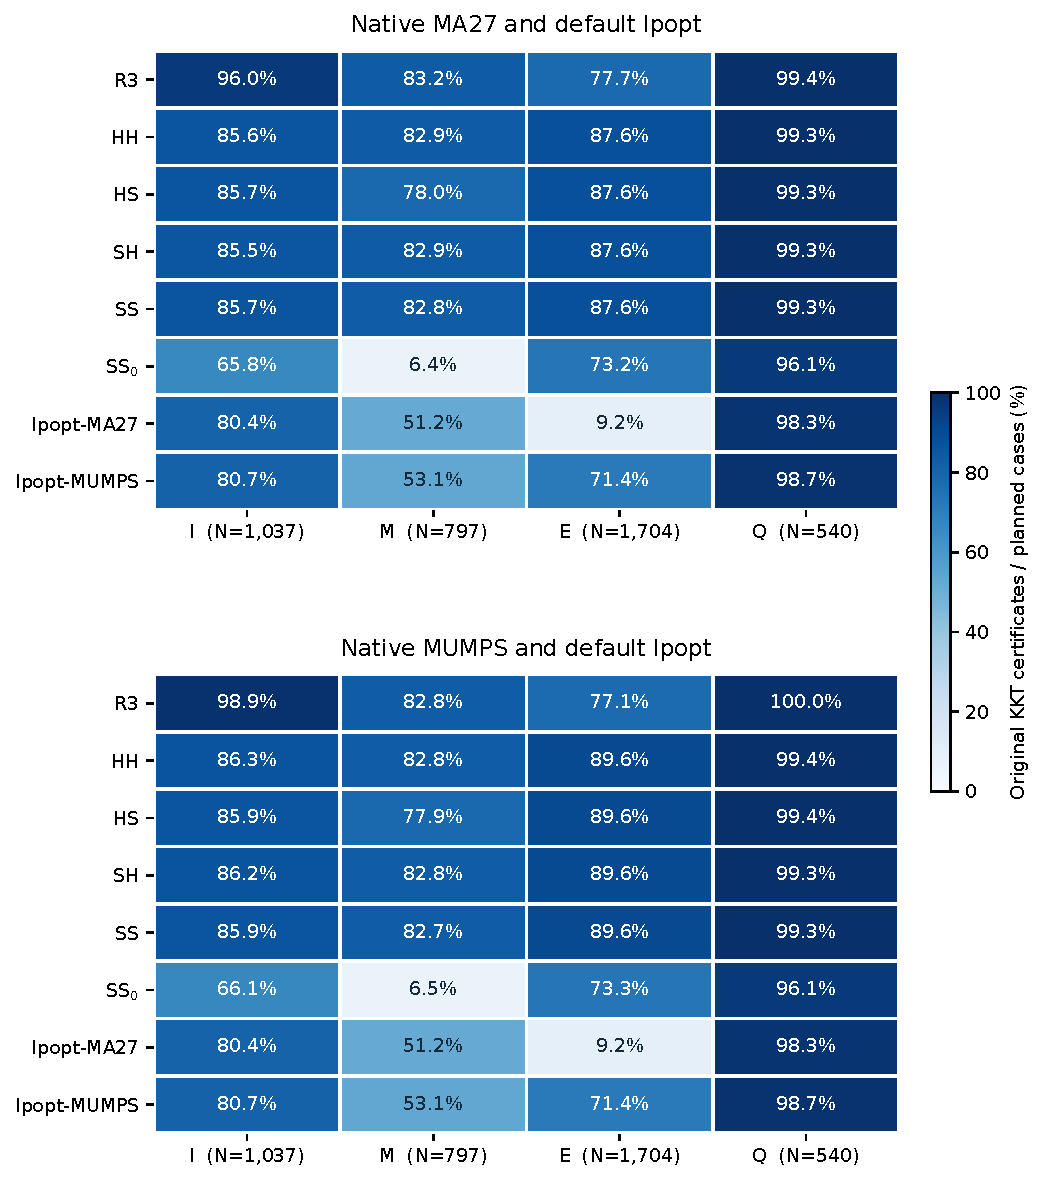
\includegraphics[width=\linewidth]{fig_current_regime_coverage.pdf}
\caption{Regime coverage with default-stopping Ipopt references.
This is a stopping-rule sensitivity display.}
\label{fig:regime-coverage}
\end{figure}

\begin{figure}[!htbp]
\centering
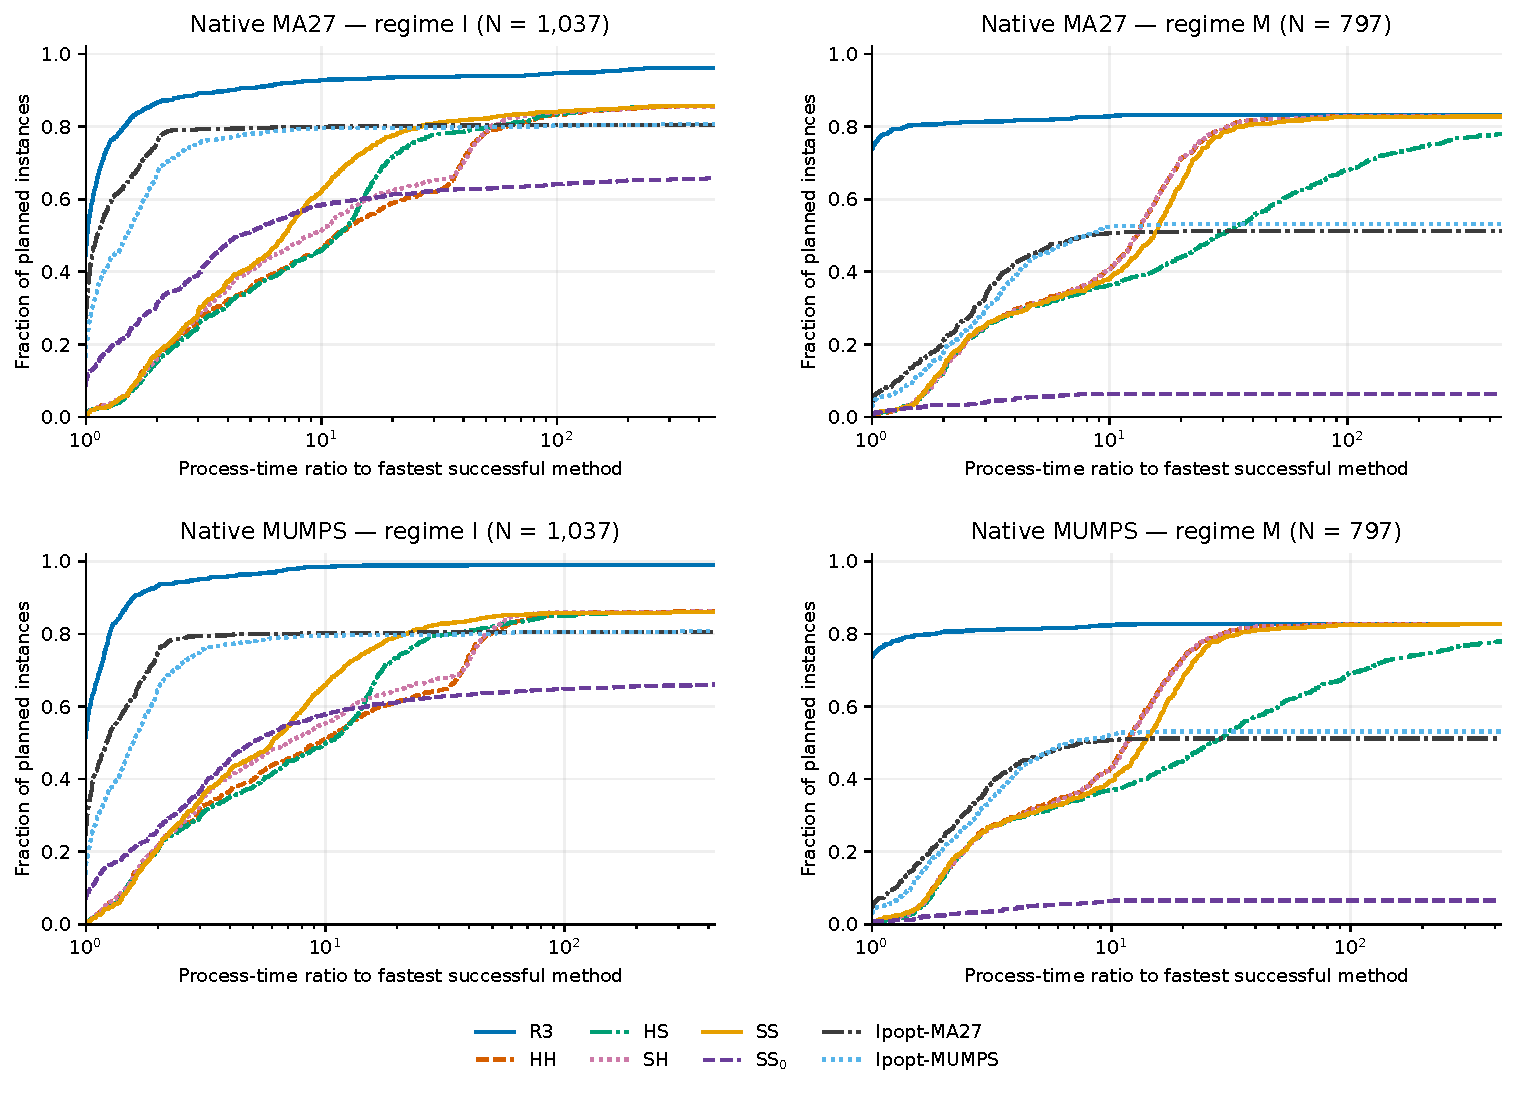
\includegraphics[width=\linewidth]{fig_core_performance_profiles_both_backends.pdf}
\caption{Elapsed-process profiles with default-stopping Ipopt references.
Failures to certify receive an infinite ratio; all planned cases remain
in each denominator. These panels complement the native-only profiles
in the main text.}
\label{fig:default-performance-profiles}
\end{figure}

\section{Mixed-regime objective distributions}\label{app:objective-M-distributions}
The signed gap is $(f_A-f_B)/\max\{1,|f_A|,|f_B|\}$, with the original
objective including its constant. Quantiles use the entire common
strict-certificate cohort. Negative gaps favor the first configuration.
The threshold triples give lower/equivalent/higher objectives at $10^{-3}$
and $10^{-2}$. Each comparison has its own paired cohort; a median of
zero and an asymmetric tail can coexist. ASU denotes the 503
radio-beamforming instances, and Other M the remaining 294 mixed problems.

\begin{table}[!htbp]
\centering\small
\caption{Complete native M threshold counts for the baseline against
every other policy, at fixed linear solver.}
\label{tab:native-M-thresholds}

% Local input expanded: native_M_objective_thresholds.tex
\begin{tabular}{@{}lllrcc@{}}
\toprule
Linear solver & Comparison & Population & $N$ & $10^{-3}$ & $10^{-2}$\\
\midrule
MA27 & R3/HH & ASU & 375 & 1/2/372 & 0/8/367\\
MA27 & R3/HH & Other M & 285 & 4/273/8 & 0/284/1\\
MA27 & R3/HS & ASU & 337 & 2/2/333 & 0/7/330\\
MA27 & R3/HS & Other M & 284 & 4/272/8 & 0/283/1\\
MA27 & R3/SH & ASU & 375 & 1/2/372 & 0/8/367\\
MA27 & R3/SH & Other M & 285 & 4/273/8 & 0/284/1\\
MA27 & R3/SS & ASU & 375 & 78/126/171 & 47/199/129\\
MA27 & R3/SS & Other M & 284 & 4/272/8 & 0/283/1\\
MA27 & R3/$SS_0$ & ASU & 0 & 0/0/0 & 0/0/0\\
MA27 & R3/$SS_0$ & Other M & 51 & 5/44/2 & 3/48/0\\
MUMPS & R3/HH & ASU & 375 & 1/2/372 & 0/8/367\\
MUMPS & R3/HH & Other M & 282 & 4/271/7 & 0/282/0\\
MUMPS & R3/HS & ASU & 337 & 2/2/333 & 0/7/330\\
MUMPS & R3/HS & Other M & 281 & 4/270/7 & 0/281/0\\
MUMPS & R3/SH & ASU & 375 & 1/2/372 & 0/8/367\\
MUMPS & R3/SH & Other M & 282 & 4/271/7 & 0/282/0\\
MUMPS & R3/SS & ASU & 375 & 77/127/171 & 47/199/129\\
MUMPS & R3/SS & Other M & 281 & 4/270/7 & 0/281/0\\
MUMPS & R3/$SS_0$ & ASU & 0 & 0/0/0 & 0/0/0\\
MUMPS & R3/$SS_0$ & Other M & 51 & 5/43/3 & 3/48/0\\
\bottomrule
\end{tabular}


\end{table}

The next four tables compare all twelve native configurations with both
default-stopping Ipopt references on common original certificates. Their
stopping rules differ, so these results describe the attained points on
those instances. Section~\ref{app:aligned-reference-results} reports the comparisons with
stopping tolerances chosen for the common certificate.

\begin{scaledtable}[!htbp]
\centering\scriptsize
\caption{Native MA27 objectives relative to default-stopping Ipopt--MA27,
by M population. Quartiles are percent gaps on all common certificates.}
\label{tab:objective-M-ma27-ref-ma27}
\resizebox{\linewidth}{!}{
% Local input expanded: objective_M_distributions_ma27_ref_ma27_default.tex
\begin{tabular}{@{}llrccc@{}}
\toprule
Population & Policy & $N$ & $Q_1$/median/$Q_3$ (\%) & $10^{-3}$ & $10^{-2}$\\
\midrule
All M & R3 & 408 & 4.474/15.374/23.054 & 10/56/342 & 4/75/329\\
 & HH & 406 & -0.222/0.000/0.324 & 118/162/126 & 44/310/52\\
 & HS & 381 & -0.191/0.000/0.346 & 105/142/134 & 50/279/52\\
 & SH & 406 & -0.222/0.000/0.324 & 118/162/126 & 44/310/52\\
 & SS & 406 & 4.482/14.184/22.375 & 13/53/340 & 4/75/327\\
 & $SS_0$ & 40 & 0.000/0.000/0.833 & 3/23/14 & 0/30/10\\
\midrule
ASU & R3 & 324 & 11.176/18.133/24.927 & 0/3/321 & 0/7/317\\
 & HH & 324 & -0.298/0.000/0.401 & 105/112/107 & 40/243/41\\
 & HS & 299 & -0.273/0.000/0.403 & 92/92/115 & 46/212/41\\
 & SH & 324 & -0.298/0.000/0.401 & 105/112/107 & 40/243/41\\
 & SS & 324 & 10.264/17.209/23.680 & 0/3/321 & 0/8/316\\
 & $SS_0$ & 0 & -- & 0/0/0 & 0/0/0\\
\midrule
Other M & R3 & 84 & 0.000/0.000/0.065 & 10/53/21 & 4/68/12\\
 & HH & 82 & 0.000/0.000/0.014 & 13/50/19 & 4/67/11\\
 & HS & 82 & 0.000/0.000/0.014 & 13/50/19 & 4/67/11\\
 & SH & 82 & 0.000/0.000/0.014 & 13/50/19 & 4/67/11\\
 & SS & 82 & 0.000/0.000/0.014 & 13/50/19 & 4/67/11\\
 & $SS_0$ & 40 & 0.000/0.000/0.833 & 3/23/14 & 0/30/10\\
\bottomrule
\end{tabular}

}
\end{scaledtable}
\begin{scaledtable}[!htbp]
\centering\scriptsize
\caption{Native MA27 objectives relative to default-stopping Ipopt--MUMPS.}
\label{tab:objective-M-ma27-ref-mumps}
\resizebox{\linewidth}{!}{
% Local input expanded: objective_M_distributions_ma27_ref_mumps_default.tex
\begin{tabular}{@{}llrccc@{}}
\toprule
Population & Policy & $N$ & $Q_1$/median/$Q_3$ (\%) & $10^{-3}$ & $10^{-2}$\\
\midrule
All M & R3 & 423 & 5.373/15.695/23.020 & 13/55/355 & 6/73/344\\
 & HH & 421 & -0.155/0.000/0.335 & 119/167/135 & 39/328/54\\
 & HS & 387 & -0.125/0.000/0.363 & 105/148/134 & 39/293/55\\
 & SH & 421 & -0.155/0.000/0.335 & 119/167/135 & 39/328/54\\
 & SS & 421 & 5.091/14.965/22.690 & 19/48/354 & 7/71/343\\
 & $SS_0$ & 40 & 0.000/0.000/0.833 & 5/21/14 & 2/28/10\\
\midrule
ASU & R3 & 341 & 11.954/18.543/24.717 & 0/5/336 & 0/7/334\\
 & HH & 341 & -0.220/0.000/0.402 & 103/120/118 & 33/263/45\\
 & HS & 307 & -0.201/0.000/0.456 & 89/101/117 & 33/228/46\\
 & SH & 341 & -0.220/0.000/0.402 & 103/120/118 & 33/263/45\\
 & SS & 341 & 11.469/17.351/23.889 & 3/1/337 & 1/6/334\\
 & $SS_0$ & 0 & -- & 0/0/0 & 0/0/0\\
\midrule
Other M & R3 & 82 & 0.000/0.000/0.041 & 13/50/19 & 6/66/10\\
 & HH & 80 & -0.009/0.000/0.010 & 16/47/17 & 6/65/9\\
 & HS & 80 & -0.009/0.000/0.010 & 16/47/17 & 6/65/9\\
 & SH & 80 & -0.009/0.000/0.010 & 16/47/17 & 6/65/9\\
 & SS & 80 & -0.009/0.000/0.010 & 16/47/17 & 6/65/9\\
 & $SS_0$ & 40 & 0.000/0.000/0.833 & 5/21/14 & 2/28/10\\
\bottomrule
\end{tabular}

}
\end{scaledtable}
\begin{scaledtable}[!htbp]
\centering\scriptsize
\caption{Native MUMPS objectives relative to default-stopping Ipopt--MA27.}
\label{tab:objective-M-mumps-ref-ma27}
\resizebox{\linewidth}{!}{
% Local input expanded: objective_M_distributions_mumps_ref_ma27_default.tex
\begin{tabular}{@{}llrccc@{}}
\toprule
Population & Policy & $N$ & $Q_1$/median/$Q_3$ (\%) & $10^{-3}$ & $10^{-2}$\\
\midrule
All M & R3 & 407 & 4.519/15.438/23.064 & 9/56/342 & 3/75/329\\
 & HH & 405 & -0.221/0.000/0.330 & 117/161/127 & 43/309/53\\
 & HS & 380 & -0.190/0.000/0.362 & 104/141/135 & 49/278/53\\
 & SH & 405 & -0.221/0.000/0.330 & 117/161/127 & 43/309/53\\
 & SS & 405 & 4.701/14.221/22.411 & 12/53/340 & 3/74/328\\
 & $SS_0$ & 41 & 0.000/0.000/0.728 & 3/24/14 & 0/31/10\\
\midrule
ASU & R3 & 324 & 11.176/18.133/24.927 & 0/3/321 & 0/7/317\\
 & HH & 324 & -0.298/0.000/0.401 & 105/112/107 & 40/243/41\\
 & HS & 299 & -0.273/0.000/0.403 & 92/92/115 & 46/212/41\\
 & SH & 324 & -0.298/0.000/0.401 & 105/112/107 & 40/243/41\\
 & SS & 324 & 10.264/17.209/23.680 & 0/4/320 & 0/8/316\\
 & $SS_0$ & 0 & -- & 0/0/0 & 0/0/0\\
\midrule
Other M & R3 & 83 & 0.000/0.000/0.086 & 9/53/21 & 3/68/12\\
 & HH & 81 & 0.000/0.000/0.046 & 12/49/20 & 3/66/12\\
 & HS & 81 & 0.000/0.000/0.046 & 12/49/20 & 3/66/12\\
 & SH & 81 & 0.000/0.000/0.046 & 12/49/20 & 3/66/12\\
 & SS & 81 & 0.000/0.000/0.046 & 12/49/20 & 3/66/12\\
 & $SS_0$ & 41 & 0.000/0.000/0.728 & 3/24/14 & 0/31/10\\
\bottomrule
\end{tabular}

}
\end{scaledtable}
\begin{scaledtable}[!htbp]
\centering\scriptsize
\caption{Native MUMPS objectives relative to default-stopping Ipopt--MUMPS.}
\label{tab:objective-M-mumps-ref-mumps}
\resizebox{\linewidth}{!}{
% Local input expanded: objective_M_distributions_mumps_ref_mumps_default.tex
\begin{tabular}{@{}llrccc@{}}
\toprule
Population & Policy & $N$ & $Q_1$/median/$Q_3$ (\%) & $10^{-3}$ & $10^{-2}$\\
\midrule
All M & R3 & 422 & 5.487/15.777/23.055 & 12/55/355 & 5/73/344\\
 & HH & 420 & -0.154/0.000/0.338 & 118/166/136 & 38/327/55\\
 & HS & 386 & -0.122/0.000/0.381 & 104/147/135 & 38/292/56\\
 & SH & 420 & -0.154/0.000/0.338 & 118/166/136 & 38/327/55\\
 & SS & 420 & 5.228/14.990/22.714 & 18/48/354 & 6/70/344\\
 & $SS_0$ & 41 & 0.000/0.000/0.728 & 5/22/14 & 2/29/10\\
\midrule
ASU & R3 & 341 & 11.954/18.543/24.717 & 0/5/336 & 0/7/334\\
 & HH & 341 & -0.220/0.000/0.402 & 103/120/118 & 33/263/45\\
 & HS & 307 & -0.201/0.000/0.456 & 89/101/117 & 33/228/46\\
 & SH & 341 & -0.220/0.000/0.402 & 103/120/118 & 33/263/45\\
 & SS & 341 & 11.469/17.351/23.889 & 3/2/336 & 1/6/334\\
 & $SS_0$ & 0 & -- & 0/0/0 & 0/0/0\\
\midrule
Other M & R3 & 81 & 0.000/0.000/0.045 & 12/50/19 & 5/66/10\\
 & HH & 79 & -0.002/0.000/0.013 & 15/46/18 & 5/64/10\\
 & HS & 79 & -0.002/0.000/0.013 & 15/46/18 & 5/64/10\\
 & SH & 79 & -0.002/0.000/0.013 & 15/46/18 & 5/64/10\\
 & SS & 79 & -0.002/0.000/0.013 & 15/46/18 & 5/64/10\\
 & $SS_0$ & 41 & 0.000/0.000/0.728 & 5/22/14 & 2/29/10\\
\bottomrule
\end{tabular}

}
\end{scaledtable}
\FloatBarrier

% Detailed blocks moved from R9's controlled examples. Existing analytical
% formulas, measurements and final point tables are preserved without recomputation.
\section{Details of the controlled comparisons}\label{supp:controlled-details}
This section gives initialization details, final results and local-rate
diagnostics for the five controlled figures.

\subsection{Common settings and first illustration}

\paragraph{A paired numerical comparison.}
We fix $\beta=0.1$ and the strictly feasible point
\[
 x^0=(10,\,15.732132722552274)^T,
 \qquad g_\beta(x^0)=-74.25.
\]
The objective is affine, so its correction is zero. The adaptive
LazyQCQP run starts with a scalar constraint correction and, after its
first accepted step, retains a single normal direction and removes the
remaining scalar term. The comparisons use the same QCQP, primal start, bound and original
tolerance $10^{-8}$.

The classical comparators are SLSQP \citep{Kraft1988}, with its own quasi Newton Hessian
update and exact analytical first derivatives, and Ipopt with exact
Lagrangian Hessians and monotone barrier updates. The controlled Ipopt
runs use $10^{-8}$ for the overall, feasibility, dual and complementarity
tolerances, disable acceptable termination, scaling and bound relaxation,
and use MUMPS. These settings support the common original $10^{-8}$ test
for the geometric illustrations. Multiplier and barrier initializations
are method-specific. A separate scalar LazyQCQP run changes only the
constraint correction family; its remaining parameter rules are shared
with the adaptive run.


All recorded points satisfy the explicit bound. The common residual
in the main text eliminates only that bound normal and uses each
method's recorded quadratic-constraint multiplier without refitting.
The bound is inactive at the solution. Final points also pass the
full original KKT test with bound multipliers in the original variables
when available.

The exact directional model is minimized at $y_2=0$ and
$y_1=(a+a^{-1})/2\geq1$. After its first update, the normal
coordinate therefore decreases to one and obeys the quadratic
recurrence in the main text, independently of $\beta$.
At a boundary point, $a^2-\beta b^2=1$, the linearized constraint is
\[
 y_1\geq\frac{1+\beta b y_2}{a}.
\]
For $b\ne0$, that halfspace contains points with $y_1=0$ that violate
the original QCQP. A regularized SQP subproblem can propose such points,
whose acceptance requires feasibility control. The upper model excludes them. At the current iterate, both Newton methods retain the
original linearized primal equations; their Hessian blocks and
globalization determine the actual trajectories.


\begin{table}[tb]
\centering\small
\caption{First illustration, \eqref{eq:favorable-family}, with $\beta=0.1$. First denotes the first accepted
iteration satisfying the common original criterion at $10^{-8}$;
reported denotes the final iteration count. Final $R$ uses the full
original KKT residual.}
\label{tab:favorable-comparison}

% Local input expanded: favorable_current.tex
\begin{tabular}{lrrr}
\toprule
Method & First & Reported & Final $R$ \\
\midrule
LazyQCQP: directional & 16 & 16 & $5.121\times10^{-9}$ \\
LazyQCQP: scalar & 56 & 56 & $5.120\times10^{-9}$ \\
SLSQP & 25 & 26 & $1.818\times10^{-13}$ \\
Ipopt: monotone & 30 & 30 & $2.509\times10^{-9}$ \\
\bottomrule
\end{tabular}


\end{table}

The iteration ordering in Table~\ref{tab:favorable-comparison} belongs
to the stated coefficients and start. The directional correction leaves
the positive $x_2$ curvature unchanged, whereas the scalar correction
also changes tangent motion. 

The repeated final LazyQCQP residual near $5.12\times10^{-9}$ also has
a specific explanation. Both configurations finish after seven barrier
updates, at $\mu=1.28\times10^{-9}$. Their complementarity is about
$1.28\times10^{-9}$ and the full stationarity residual is about
$5.12\times10^{-9}$. The stopping point therefore reflects the common
barrier schedule as well as the curvature model. This value of $\mu$
is above the prescribed floor; the repeated number is not evidence
that a complementarity floor was reached. Iteration counts in this
comparison include the work of moving between barrier stages.

\subsection{Coordinate normalization}

For $\beta=0.1$, the analytically equivalent coordinates
$u=x_1$, $w=\sqrt\beta\,x_2$ give
$1-u^2+w^2\leq0$. We transformed the prescribed primal start
and lifted every terminal point and multiplier back to the original
coordinates for certification. Table~\ref{tab:normalization-control}
reports a separate run with the same settings. The round-trip error of
the double-precision start is $1.78\times10^{-15}$.

\begin{table}[!htbp]
\centering\small
\caption{Normalization of the first illustration. Major iterations and
original-coordinate residuals $\mathcal R$ before and after the change
of variables. Every displayed final point meets the common original
criterion.}
\label{tab:normalization-control}

% Local input expanded: normalization.tex
\begin{tabular}{lrrrr}
\toprule
Method & Original & Normalized & Original $\mathcal R$ & Lifted $\mathcal R$ \\
\midrule
LazyQCQP directional & 16 & 16 & $5.12\times10^{-9}$ & $5.12\times10^{-9}$ \\
LazyQCQP scalar & 56 & 30 & $5.12\times10^{-9}$ & $2.20\times10^{-9}$ \\
SLSQP & 26 & 17 & $1.82\times10^{-13}$ & $1.20\times10^{-11}$ \\
Ipopt monotone & 30 & 15 & $2.51\times10^{-9}$ & $2.51\times10^{-9}$ \\
\bottomrule
\end{tabular}


\end{table}

Directional correction takes 16 iterations in both representations,
whereas the scalar correction changes from 56 to 30. Monotone Ipopt
and SLSQP also use fewer iterations. All four final points after normalization
meet the original $10^{-8}$ threshold.
The scalar correction $2I$ in the normalized coordinates lifts to
$\operatorname{diag}(2,2\beta)$ in the original coordinates.
At the solution, its tangent excess and true tangent Hessian are both
$\beta$, so the exact-model factor becomes $1/2$, compared with
$10/11$ for the original scalar correction. The directional correction
$\operatorname{diag}(2,0)$ is preserved. These factors describe
stationary models; the finite iteration counts also depend on the
barrier and globalization. In particular, the infinity-norm stopping
tests and coordinate-dependent numerical rules can change under an equivalent
representation.

\subsection{A fixed radial geometry across dimensions}

The same geometry extends to
\begin{equation}\label{eq:radial-family}
 \min_{u\in\mathbb R,\,v\in\mathbb R^{n-1}} u
 \quad\text{subject to}\quad
 1-u^2+\beta\|v\|^2\leq0,\qquad u\geq0,
 \qquad \beta=0.1.
\end{equation}
The feasible set satisfies $u\geq\sqrt{1+\beta\|v\|^2}$, so its
unique global minimizer is $(1,0)$, with inequality multiplier $1/2$.
The quadratic constraint Hessian has one negative eigenvalue for every
$n$. The correction $\operatorname{diag}(2,0_{n-1})$ therefore has rank
one independently of dimension. It preserves all positive tangent
curvature, and exact minimization of its upper model gives
\[
 (u,v)\longmapsto\left(\frac{u+u^{-1}}2,0\right),\qquad
 u^+-1=\frac{(u-1)^2}{2u}.
\]
This is the analytical reference map; the computed LazyQCQP trajectory
also includes barrier and globalization effects.
The mathematical family has no finite coordinate bounds on $v$ and is
rotationally invariant in $v$. An orthogonal change of
coordinates can place $v$ on one axis, reducing the optimization geometry
to the two variables $u$ and $\|v\|$. Increasing $n$ therefore tests the
cost of representing and solving this fixed radial structure, not a
growing number of geometrically distinct decisions. The prescribed
uniform starts also lie in a two dimensional symmetric subspace.
The implementation uses coordinate-dependent infinity-norm stopping
and control rules. These, together with rounding and parameter updates,
permit iteration counts to vary with dimension despite the rotationally
invariant radial model.

For all dimensions we prescribe
\[
 u^0=10,\qquad
 v_j^0=\frac{r}{\sqrt{n-1}},\qquad
 r=\tfrac12\sqrt{990},
\]
with the realized starting vectors fixed before the runs. Thus the
initial radial geometry is unchanged, and the original constraint
value is approximately $-74.25$. There is one quadratic inequality,
one lower bound and no equality. All final points satisfy the original
unscaled KKT threshold $10^{-8}$.

Figure~\ref{fig:radial-scaling} reports all tested dimensions, including
the small cases on which SLSQP is faster in elapsed time. The scalar
and directional LazyQCQP curves share the same numerical rules. Five solves
per method and dimension use one pinned CPU and one numerical thread.
The time measurements
exclude process startup and problem-description preparation. The
SLSQP comparison uses its existing multipliers at accepted points and
stops when an independent original KKT test meets the common threshold;
this checking work is included. Its steps before that stop match the
corresponding uninterrupted SLSQP trajectory exactly. Ipopt uses the
controlled monotone settings stated above.

\begin{scaledtable}[tb]
\centering\small
\caption{Median numerical solve times in milliseconds over five solves
of \eqref{eq:radial-family}, with major iterations in parentheses.
All final points satisfy the original KKT tolerance $10^{-8}$.}
\label{tab:radial-times}
\resizebox{\linewidth}{!}{
% Local input expanded: radial_times.tex
\begin{tabular}{rrrrr}
\toprule
$n$ & \shortstack{HH\\directional} & \shortstack{HS\\scalar} & \shortstack{Ipopt\\monotone} & SLSQP \\
\midrule
2 & 3.339 (16) & 6.196 (56) & 8.200 (30) & 2.156 (25) \\
10 & 4.484 (16) & 8.342 (58) & 9.089 (30) & 1.191 (22) \\
50 & 6.090 (16) & 20.284 (59) & 12.674 (30) & 1.435 (22) \\
100 & 8.199 (16) & 37.519 (64) & 16.467 (30) & 2.457 (22) \\
200 & 12.807 (16) & 43.293 (68) & 23.376 (30) & 4.824 (24) \\
500 & 29.293 (16) & 93.824 (70) & 47.562 (30) & 16.692 (22) \\
1000 & 45.193 (16) & 219.545 (92) & 93.725 (30) & 97.398 (22) \\
2000 & 106.408 (16) & 426.544 (80) & 172.542 (30) & 429.261 (23) \\
\bottomrule
\end{tabular}

}
\end{scaledtable}


At $n=2000$, the directional configuration takes 16 major iterations
and has median time 106.41 ms, compared with 80 iterations and
426.54 ms for the scalar configuration. Monotone Ipopt takes
172.54 ms and SLSQP 429.26 ms.
The measured speedups are 1.62 relative to Ipopt
and 4.03 relative to SLSQP. All five directional
times are below every measured comparator time at this dimension.
SLSQP uses a dense quasi Newton representation, whereas the quadratic
structure here supports sparse direct equations. The observed times
reflect the combined iteration counts, storage choices and linear-algebra
implementations; their separate contributions were not measured.
These costs concern the stated radial family, coordinates and numerical rules. The paired problems in the main text examine
a geometry in which tangent majorization slows progress.

\subsection{Exact reference geometry for the paired problems}
The paired problems have the common start $x^0=(1.6,0.8)^\top$,
unique global solution $x^*=(1,0)^\top$, value $f_a(x^*)=0.405$ and
multiplier $\lambda^*=(1-a)/2=0.45$.
The unconstrained minimizer $(a,0)^\top$ lies in the excluded region of
both problems, so the constraint must be active at the constrained
solution. The objective measures squared distance from this point.
For $g_-$, the solution claim follows by writing $x=r(\cos\theta,\sin\theta)$:
$r\geq1$ and
$f_a(x)\geq\tfrac12(r-a)^2\geq\tfrac12(1-a)^2$,
with equality only at $x^*$.
For $g_+$, feasibility implies $|x_1|\geq\sqrt{1+x_2^2}\geq1$;
$x_1\geq1$ gives the same lower bound, while $x_1\leq-1$ gives a
strictly larger value. Both solutions satisfy LICQ, strict
complementarity, and the second order sufficient condition.

For the circular exclusion, projection onto the exact affine majorant
from the main text gives, in a neighbourhood of $x^*$,
\begin{equation}
 T_-(x)=ae_1+\frac{(1+\|x\|^2)/2-ax_1}{\|x\|^2}x,
 \qquad
 DT_-(x^*)=\operatorname{diag}(0,1-a).
 \label{eq:circle-map}
\end{equation}
For every feasible iterate with $x_1>0$, the projection coefficient in
\eqref{eq:circle-map} is positive, the next point has first coordinate
at least $a$, and the current iterate is feasible for the model. Strong convexity gives
$f_a(x)-f_a(T_-(x))\geq\tfrac12\|T_-(x)-x\|^2$.

The objective sublevel set is compact and the model multipliers are
bounded, since $\|x\|\geq1$. Theorem~\ref{thm:theory-cluster}
therefore applies to the exact reference iteration. Its only KKT
accumulation point with $x_1\geq a$ is $x^*$, so the full sequence
converges to $x^*$. The tangential error then contracts linearly with
factor $0.9$.
The factor has a direct curvature interpretation. At the solution,
\[
 H_T=1-2\lambda^*=a=0.1,\qquad
 E_T=2\lambda^*=1-a=0.9,\qquad B_T=H_T+E_T=1.
\]
Thus the local majorant factor is $E_T/B_T=0.9$, as predicted by
Theorem~\ref{thm:smooth-anchored-map}. The correction is already the
minimal spectral correction for this concave quadratic. Its validity and accurate
spectral construction do not remove the tangent gap.

The first-order Taylor constraint of the circular QCQP is precisely
its affine majorant. Exact-Hessian SQP uses the original signed
Lagrangian curvature $aI$, whereas exact minimization of the majorant
keeps the convex objective Hessian $I$.

\subsection{Final residuals and curvature diagnostics}

We compare LazyQCQP with the classical primal and dual interior point
method Ipopt~\cite{WachterBiegler2006}, using exact derivatives and
its exact Lagrangian Hessian. For the circular problem an exact-Hessian
SQP reference solves the one-inequality quadratic subproblem analytically
and uses an Armijo line search. All methods use the same primal start.
We write $R$ for the independently evaluated, unscaled original residual
\eqref{eq:kkt-residual} and require $R\leq10^{-8}$.

\Needspace{7\baselineskip}
Natural dual and barrier initializations are method-specific.
The scalar and adaptive configurations
start with the same scalar correction. On $g_+$ the adaptive
construction subsequently retains one normal direction and removes
the residual scalar term; on $g_-$ it preserves the minimal scalar
correction. The exact-majorant curves are analytical reference iterations;
the remaining curves are runs of the numerical implementation.
The adaptive hyperbolic run has an original primal violation of about
$0.493$ at its third accepted iterate, despite the feasible start.
The original-function globalization accommodates this intermediate
violation.


\begin{table}[tb]
\centering\small
\caption{Accepted iterations and final original KKT residual for the paired
problems, from the common primal start $(1.6,0.8)^T$ and tolerance $10^{-8}$.
The scalar and adaptive policies have identical circular trajectories.
The SQP reference is evaluated on the circular problem only.}
\label{tab:toy-comparison}
\begin{tabular}{lrrrr}
\toprule
&\multicolumn{2}{c}{Circular exclusion}&\multicolumn{2}{c}{Hyperbolic exclusion}\\
Method&Iterations&$R$&Iterations&$R$\\
\midrule
LazyQCQP, scalar&146&$9.96\,10^{-9}$&20&$3.75\,10^{-9}$\\
LazyQCQP, adaptive&146&$9.96\,10^{-9}$&14&$5.12\,10^{-9}$\\
Exact-Hessian SQP reference&7&$9.91\,10^{-14}$&\multicolumn{2}{c}{---}\\
Ipopt, exact Hessian&6&$1.15\,10^{-9}$&4&$1.25\,10^{-10}$\\
Exact majorant reference&147&$9.06\,10^{-9}$&5&$1.16\,10^{-10}$\\
\bottomrule
\end{tabular}
\end{table}

The example identifies both the benefit of selective curvature and a
regime in which an exact-curvature method retains a local advantage.

The computed trajectories give a direct check of the rate
formula. Table~\ref{tab:toy-curvature-rates} uses $H_T$ and $E_T$
computed analytically at the known solution, independently of the
observed quotients. The scalar trajectory of the first illustration has
median tangent ratio $0.909091$ over iterations 39 through 49, consistent
with its analytically predicted factor $10/11$. On the circle, both the exact reference and the
computed adaptive trajectory have a median tangent error ratio of
$0.9000$ over iterations 40 through 120. On the hyperbola, the scalar
trajectory has ratio $0.321429$ in its last five steps, matching $9/28$.
The directional exact map instead has quadratic normal error, with
$e_{1,k+1}/e_{1,k}^2$ approaching $1/2$.

\begin{table}[tb]
\centering\small
\caption{Curvature diagnostics for the regular toy solutions.
$H_T,E_T,\kappa$ and the linearized model factor are analytical values.
Observed quantities are measured from the computed trajectories, with
$e_{1,k}=x_{1,k}-1$. They are not fitted to obtain $\kappa$.}
\label{tab:toy-curvature-rates}
\begin{tabularx}{\linewidth}{@{}lrrrr>{\raggedright\arraybackslash}X@{}}
\toprule
Geometry and trajectory & $H_T$ & $E_T$ & $\kappa$ & $\rho(T_*)$ & Observed quantity\\
\midrule
\shortstack[l]{First illustration\\scalar} & $0.1$ & $1$ & $10$ & $10/11$
 & Median $|x_{2,k}/x_{2,k-1}|=0.909091$, $39\leq k\leq49$.\\
\shortstack[l]{Circle\\adaptive} & $0.1$ & $0.9$ & $9$ & $0.9$
 & Median $|x_{2,k+1}/x_{2,k}|=0.9000$, $40\leq k<120$.\\
\shortstack[l]{Hyperbola\\scalar} & $1.9$ & $0.9$ & $9/19$ & $9/28$
 & Median $|x_{2,k+1}/x_{2,k}|=0.321429$, $15\leq k<20$.\\
\shortstack[l]{Hyperbola\\exact directional} & $1.9$ & $0$ & $0$ & $0$
 & $e_{1,4}/e_{1,3}^2=0.499992$; normal error is quadratic.\\
\shortstack[l]{Hyperbola\\adaptive} & $1.9$ & $0$ & $0$ & $0$
 & Median $|e_{1,k+1}/e_{1,k}|=0.2000$, $9\leq k<14$.\\
\bottomrule
\end{tabularx}
\end{table}

The last row distinguishes the model map from the barrier trajectory. In the adaptive hyperbolic run the final barrier parameter
is $1.28\times10^{-9}$ after seven reductions, with complementarity
about $1.28\times10^{-9}$ and stationarity about $5.12\times10^{-9}$.
Its final normal error follows the barrier reduction factor $0.2$;
the barrier perturbation is not negligible relative to that error.
Consequently the zero linear term of the exact directional map does
not predict a quadratic rate for this finite computed tail. The
comparison supports the role of tangent correction while making the
barrier forcing condition observable.

\FloatBarrier
\section{Composition sensitivity in every regime}\label{app:composition}
Instance coverage weights each planned QCQP equally. We also average
coverage rates across families and collections, with equal weight for
each nonempty group within its partition. An additional summary excludes the largest collection in each regime. Every planned instance stays in the corresponding denominator,
including failures caused by execution or audit incidents.
These are descriptive corpus summaries; groups are not treated as independent
statistical repetitions.

% Keep the compact composition table with its introductory section.
% The compact metadata table describes the common structural partitions.
\begingroup
\renewenvironment{table*}[1][]{\begin{table}[!htbp]}{\end{table}}

% Local input expanded: composition_all.tex
\begin{scaledtable}[!htbp]
\centering
\caption{Composition of every observed regime. Dataset and explicit-family partitions are kept separate. Parentheses show the share of all cases in the regime (\%).}
\label{tab:composition-all-regimes}
\footnotesize
\setlength{\tabcolsep}{3pt}
\resizebox{\linewidth}{!}{\begin{tabular}{lrrrlrlr}
\toprule
Regime & $N$ & Datasets & Families & \shortstack{Largest\\dataset} & $n$ (\%) & \shortstack{Largest explicit\\family} & $n$ (\%) \\
\midrule
I & 1037 & 16 & 15 & \shortstack[l]{IJOC partition\\QCQP} & 150 (14.46) & \shortstack[l]{IJOC partition\\QCQP} & 150 (14.46) \\
M & 797 & 11 & 6 & \shortstack[l]{ASU radio-\\beamforming} & 503 (63.11) & \shortstack[l]{Application\\models} & 530 (66.50) \\
E & 1704 & 7 & 4 & GasLib134 & 1208 (70.89) & GasLib134 & 1208 (70.89) \\
Q & 540 & 4 & 3 & Robot arm & 500 (92.59) & \shortstack[l]{Application\\models} & 503 (93.15) \\
\bottomrule
\end{tabular}}
\par\smallskip
\begin{minipage}{0.97\textwidth}
\footnotesize Explicit family and dataset labels are present for every case; neither partition contains missing or unknown labels. Family names are taken directly from the fixed metadata, without substituting dataset labels. The broad family \shortstack[l]{Application\\models} includes several datasets.
\end{minipage}
\end{scaledtable}


\endgroup

\begin{scaledtable}[!htbp]
\centering\small
\caption{Coverage sensitivity for native MA27 policies and both Ipopt barrier strategies with MA27 and certificate-matched stopping targets.}
\label{tab:balance-native-ma27}
\resizebox{\linewidth}{!}{
% Local input expanded: coverage_balance_native_ma27.tex
\begin{tabular}{@{}lrrrr@{}}
\toprule
Policy & Instance (\%) & Family macro (\%) & Collection macro (\%) & Outside largest (\%) \\
\midrule
\multicolumn{5}{l}{\textbf{Regime I}: outside IJOC partition QCQP ($N=887$).} \\
R3 & 96.05 & 88.44 & 89.17 & 95.38 \\
HH & 85.63 & 80.76 & 82.25 & 83.20 \\
HS & 85.73 & 80.40 & 82.20 & 83.31 \\
SH & 85.54 & 80.63 & 82.13 & 83.09 \\
SS & 85.73 & 80.40 & 82.20 & 83.31 \\
$SS_0$ & 65.77 & 57.81 & 52.12 & 59.98 \\
Ipopt monotone & 97.20 & 89.87 & 84.60 & 96.73 \\
Ipopt adaptive & 95.37 & 91.87 & 91.16 & 94.59 \\
\midrule
\multicolumn{5}{l}{\textbf{Regime M}: outside ASU radio-beamforming ($N=294$).} \\
R3 & 83.19 & 91.55 & 86.23 & 97.96 \\
HH & 82.94 & 91.48 & 76.61 & 97.28 \\
HS & 78.04 & 86.12 & 73.65 & 96.94 \\
SH & 82.94 & 91.48 & 76.61 & 97.28 \\
SS & 82.81 & 87.32 & 74.33 & 96.94 \\
$SS_0$ & 6.40 & 23.09 & 28.22 & 17.35 \\
Ipopt monotone & 54.96 & 81.52 & 70.55 & 76.87 \\
Ipopt adaptive & 42.16 & 77.80 & 68.39 & 94.56 \\
\midrule
\multicolumn{5}{l}{\textbf{Regime E}: outside GasLib134 ($N=496$).} \\
R3 & 77.70 & 64.11 & 67.66 & 23.39 \\
HH & 87.56 & 80.21 & 81.75 & 57.26 \\
HS & 87.56 & 80.21 & 81.75 & 57.26 \\
SH & 87.56 & 80.21 & 81.75 & 57.26 \\
SS & 87.56 & 80.21 & 81.75 & 57.26 \\
$SS_0$ & 73.24 & 47.06 & 40.17 & 8.06 \\
Ipopt monotone & 87.15 & 70.80 & 70.75 & 60.48 \\
Ipopt adaptive & 80.58 & 66.37 & 66.60 & 37.90 \\
\midrule
\multicolumn{5}{l}{\textbf{Regime Q}: outside Robot arm ($N=40$).} \\
R3 & 99.44 & 96.97 & 97.73 & 92.50 \\
HH & 99.26 & 95.96 & 96.97 & 90.00 \\
HS & 99.26 & 95.96 & 96.97 & 90.00 \\
SH & 99.26 & 95.96 & 96.97 & 90.00 \\
SS & 99.26 & 95.96 & 96.97 & 90.00 \\
$SS_0$ & 96.11 & 59.65 & 44.89 & 47.50 \\
Ipopt monotone & 98.89 & 93.94 & 95.45 & 85.00 \\
Ipopt adaptive & 99.44 & 96.97 & 97.73 & 92.50 \\
\bottomrule
\end{tabular}

}
\end{scaledtable}

\begin{scaledtable}[!htbp]
\centering\small
\caption{Coverage sensitivity for native MUMPS policies and both Ipopt barrier strategies with MUMPS and certificate-matched stopping targets. The weighting units and omissions match Table~\ref{tab:balance-native-ma27}.}
\label{tab:balance-native-mumps}
\resizebox{\linewidth}{!}{
% Local input expanded: coverage_balance_native_mumps.tex
\begin{tabular}{@{}lrrrr@{}}
\toprule
Policy & Instance (\%) & Family macro (\%) & Collection macro (\%) & Outside largest (\%) \\
\midrule
\multicolumn{5}{l}{\textbf{Regime I}: outside IJOC partition QCQP ($N=887$).} \\
R3 & 98.94 & 91.49 & 92.02 & 98.76 \\
HH & 86.31 & 82.27 & 83.66 & 83.99 \\
HS & 85.92 & 79.48 & 81.35 & 83.54 \\
SH & 86.21 & 82.14 & 83.54 & 83.88 \\
SS & 85.92 & 79.48 & 81.35 & 83.54 \\
$SS_0$ & 66.06 & 58.31 & 58.50 & 60.32 \\
Ipopt monotone & 97.11 & 88.81 & 83.62 & 96.62 \\
Ipopt adaptive & 95.37 & 90.28 & 82.55 & 94.59 \\
\midrule
\multicolumn{5}{l}{\textbf{Regime M}: outside ASU radio-beamforming ($N=294$).} \\
R3 & 82.81 & 91.40 & 83.38 & 96.94 \\
HH & 82.81 & 95.59 & 76.07 & 96.94 \\
HS & 77.92 & 90.22 & 73.11 & 96.60 \\
SH & 82.81 & 95.59 & 76.07 & 96.94 \\
SS & 82.69 & 91.42 & 73.80 & 96.60 \\
$SS_0$ & 6.52 & 23.13 & 28.75 & 17.69 \\
Ipopt monotone & 53.07 & 80.98 & 70.26 & 71.09 \\
Ipopt adaptive & 38.90 & 83.05 & 71.76 & 86.73 \\
\midrule
\multicolumn{5}{l}{\textbf{Regime E}: outside GasLib134 ($N=496$).} \\
R3 & 77.11 & 63.36 & 65.37 & 21.37 \\
HH & 89.61 & 85.52 & 86.56 & 64.52 \\
HS & 89.61 & 85.52 & 86.56 & 64.52 \\
SH & 89.61 & 85.52 & 86.56 & 64.52 \\
SS & 89.61 & 85.52 & 86.56 & 64.52 \\
$SS_0$ & 73.30 & 47.61 & 40.48 & 8.27 \\
Ipopt monotone & 67.66 & 66.13 & 68.19 & 64.52 \\
Ipopt adaptive & 78.40 & 71.62 & 70.11 & 70.16 \\
\midrule
\multicolumn{5}{l}{\textbf{Regime Q}: outside Robot arm ($N=40$).} \\
R3 & 100.00 & 100.00 & 100.00 & 100.00 \\
HH & 99.44 & 96.97 & 97.73 & 92.50 \\
HS & 99.44 & 96.97 & 97.73 & 92.50 \\
SH & 99.26 & 95.96 & 96.97 & 90.00 \\
SS & 99.26 & 95.96 & 96.97 & 90.00 \\
$SS_0$ & 96.11 & 59.65 & 44.89 & 47.50 \\
Ipopt monotone & 99.26 & 95.96 & 96.97 & 90.00 \\
Ipopt adaptive & 99.44 & 96.97 & 97.73 & 92.50 \\
\bottomrule
\end{tabular}

}
\end{scaledtable}


\FloatBarrier
\section{Objective thresholds and final accuracy}\label{app:objective-accuracy}
The tables compare each native backend with both default Ipopt references
on common strict certificates, using the symmetric objective gap defined
in the main text. Triples count lower/equivalent/higher objectives at the
displayed threshold. Original residuals assess final accuracy; the KKT
classifications are unchanged.

\begin{table}[!htbp]
\centering\small
\caption{Native MA27 objectives relative to default Ipopt--MA27.}
\label{tab:thresholds-ma27}

% Local input expanded: thresholds_native_ma27_ref_MA27.tex
\begin{tabular}{lrrrr}
\toprule
Policy & $N$ & $10^{-4}$ & $10^{-3}$ & $10^{-2}$ \\
\midrule
\multicolumn{5}{l}{\textbf{Regime I}} \\
R3 & 803 & 70/556/177 & 61/610/132 & 36/677/90 \\
HH & 783 & 74/524/185 & 66/586/131 & 47/647/89 \\
HS & 782 & 74/526/182 & 66/591/125 & 47/648/87 \\
SH & 783 & 73/535/175 & 66/595/122 & 47/654/82 \\
SS & 782 & 73/537/172 & 66/599/117 & 47/654/81 \\
$SS_0$ & 677 & 60/484/133 & 52/520/105 & 36/578/63 \\
\midrule
\multicolumn{5}{l}{\textbf{Regime M}} \\
R3 & 408 & 15/44/349 & 10/56/342 & 4/75/329 \\
HH & 406 & 143/103/160 & 118/162/126 & 44/310/52 \\
HS & 381 & 120/105/156 & 105/142/134 & 50/279/52 \\
SH & 406 & 143/103/160 & 118/162/126 & 44/310/52 \\
SS & 406 & 20/43/343 & 13/53/340 & 4/75/327 \\
$SS_0$ & 40 & 4/22/14 & 3/23/14 & 0/30/10 \\
\midrule
\multicolumn{5}{l}{\textbf{Regime E}} \\
R3 & 124 & 6/115/3 & 6/115/3 & 2/121/1 \\
HH & 134 & 15/112/7 & 15/118/1 & 9/124/1 \\
HS & 134 & 15/112/7 & 15/118/1 & 9/124/1 \\
SH & 134 & 15/112/7 & 15/118/1 & 9/124/1 \\
SS & 134 & 15/112/7 & 15/118/1 & 9/124/1 \\
$SS_0$ & 89 & 0/88/1 & 0/88/1 & 0/88/1 \\
\midrule
\multicolumn{5}{l}{\textbf{Regime Q}} \\
R3 & 530 & 1/525/4 & 1/526/3 & 1/527/2 \\
HH & 530 & 1/525/4 & 1/526/3 & 1/527/2 \\
HS & 530 & 1/525/4 & 1/526/3 & 1/527/2 \\
SH & 530 & 1/525/4 & 1/526/3 & 1/527/2 \\
SS & 530 & 1/525/4 & 1/526/3 & 1/527/2 \\
$SS_0$ & 517 & 1/514/2 & 1/514/2 & 1/514/2 \\
\bottomrule
\end{tabular}


\end{table}

\begin{table}[!htbp]
\centering\small
\caption{Native MA27 objectives relative to default Ipopt--MUMPS.}
\label{tab:thresholds-mumps}

% Local input expanded: thresholds_native_ma27_ref_MUMPS.tex
\begin{tabular}{lrrrr}
\toprule
Policy & $N$ & $10^{-4}$ & $10^{-3}$ & $10^{-2}$ \\
\midrule
\multicolumn{5}{l}{\textbf{Regime I}} \\
R3 & 806 & 70/557/179 & 61/611/134 & 36/680/90 \\
HH & 785 & 74/524/187 & 66/587/132 & 47/649/89 \\
HS & 784 & 74/526/184 & 66/592/126 & 47/650/87 \\
SH & 785 & 73/535/177 & 66/596/123 & 47/656/82 \\
SS & 784 & 73/537/174 & 66/600/118 & 47/656/81 \\
$SS_0$ & 678 & 60/485/133 & 52/521/105 & 36/579/63 \\
\midrule
\multicolumn{5}{l}{\textbf{Regime M}} \\
R3 & 423 & 18/41/364 & 13/55/355 & 6/73/344 \\
HH & 421 & 144/106/171 & 119/167/135 & 39/328/54 \\
HS & 387 & 122/105/160 & 105/148/134 & 39/293/55 \\
SH & 421 & 144/106/171 & 119/167/135 & 39/328/54 \\
SS & 421 & 24/40/357 & 19/48/354 & 7/71/343 \\
$SS_0$ & 40 & 6/20/14 & 5/21/14 & 2/28/10 \\
\midrule
\multicolumn{5}{l}{\textbf{Regime E}} \\
R3 & 1171 & 4/1163/4 & 4/1163/4 & 2/1167/2 \\
HH & 1188 & 17/1161/10 & 17/1166/5 & 12/1172/4 \\
HS & 1188 & 17/1161/10 & 17/1166/5 & 12/1172/4 \\
SH & 1188 & 17/1161/10 & 17/1166/5 & 12/1172/4 \\
SS & 1188 & 17/1161/10 & 17/1166/5 & 12/1172/4 \\
$SS_0$ & 1138 & 0/1137/1 & 0/1137/1 & 0/1137/1 \\
\midrule
\multicolumn{5}{l}{\textbf{Regime Q}} \\
R3 & 531 & 1/526/4 & 1/527/3 & 1/528/2 \\
HH & 531 & 1/526/4 & 1/527/3 & 1/528/2 \\
HS & 531 & 1/526/4 & 1/527/3 & 1/528/2 \\
SH & 531 & 1/526/4 & 1/527/3 & 1/528/2 \\
SS & 531 & 1/526/4 & 1/527/3 & 1/528/2 \\
$SS_0$ & 517 & 1/514/2 & 1/514/2 & 1/514/2 \\
\bottomrule
\end{tabular}


\end{table}

\begin{table}[!htbp]
\centering\small
\caption{Native MUMPS objectives relative to default Ipopt--MA27.}
\label{tab:thresholds-native-mumps-ma27}

% Local input expanded: thresholds_native_mumps_ref_MA27.tex
\begin{tabular}{lrrrr}
\toprule
Policy & $N$ & $10^{-4}$ & $10^{-3}$ & $10^{-2}$ \\
\midrule
\multicolumn{5}{l}{\textbf{Regime I}} \\
R3 & 832 & 70/514/248 & 61/631/140 & 36/706/90 \\
HH & 787 & 73/491/223 & 65/591/131 & 46/652/89 \\
HS & 785 & 74/492/219 & 66/595/124 & 47/651/87 \\
SH & 787 & 72/502/213 & 65/600/122 & 46/659/82 \\
SS & 785 & 73/503/209 & 66/603/116 & 47/657/81 \\
$SS_0$ & 679 & 60/486/133 & 52/522/105 & 37/579/63 \\
\midrule
\multicolumn{5}{l}{\textbf{Regime M}} \\
R3 & 407 & 13/44/350 & 9/56/342 & 3/75/329 \\
HH & 405 & 142/102/161 & 117/161/127 & 43/309/53 \\
HS & 380 & 119/104/157 & 104/141/135 & 49/278/53 \\
SH & 405 & 142/102/161 & 117/161/127 & 43/309/53 \\
SS & 405 & 19/42/344 & 12/53/340 & 3/74/328 \\
$SS_0$ & 41 & 4/23/14 & 3/24/14 & 0/31/10 \\
\midrule
\multicolumn{5}{l}{\textbf{Regime E}} \\
R3 & 122 & 6/113/3 & 6/113/3 & 2/119/1 \\
HH & 137 & 13/113/11 & 13/120/4 & 8/126/3 \\
HS & 137 & 13/113/11 & 13/120/4 & 8/126/3 \\
SH & 137 & 13/113/11 & 13/120/4 & 8/126/3 \\
SS & 137 & 13/113/11 & 13/120/4 & 8/126/3 \\
$SS_0$ & 89 & 0/88/1 & 0/88/1 & 0/88/1 \\
\midrule
\multicolumn{5}{l}{\textbf{Regime Q}} \\
R3 & 531 & 2/525/4 & 2/526/3 & 2/527/2 \\
HH & 531 & 2/525/4 & 2/526/3 & 2/527/2 \\
HS & 531 & 2/525/4 & 2/526/3 & 2/527/2 \\
SH & 530 & 1/525/4 & 1/526/3 & 1/527/2 \\
SS & 530 & 1/525/4 & 1/526/3 & 1/527/2 \\
$SS_0$ & 517 & 1/514/2 & 1/514/2 & 1/514/2 \\
\bottomrule
\end{tabular}


\end{table}

\begin{table}[!htbp]
\centering\small
\caption{Native MUMPS objectives relative to default Ipopt--MUMPS.}
\label{tab:thresholds-native-mumps-mumps}

% Local input expanded: thresholds_native_mumps_ref_MUMPS.tex
\begin{tabular}{lrrrr}
\toprule
Policy & $N$ & $10^{-4}$ & $10^{-3}$ & $10^{-2}$ \\
\midrule
\multicolumn{5}{l}{\textbf{Regime I}} \\
R3 & 835 & 70/515/250 & 61/632/142 & 36/709/90 \\
HH & 789 & 73/491/225 & 65/592/132 & 46/654/89 \\
HS & 787 & 74/492/221 & 66/596/125 & 47/653/87 \\
SH & 789 & 72/502/215 & 65/601/123 & 46/661/82 \\
SS & 787 & 73/503/211 & 66/604/117 & 47/659/81 \\
$SS_0$ & 680 & 60/487/133 & 52/523/105 & 37/580/63 \\
\midrule
\multicolumn{5}{l}{\textbf{Regime M}} \\
R3 & 422 & 16/41/365 & 12/55/355 & 5/73/344 \\
HH & 420 & 143/105/172 & 118/166/136 & 38/327/55 \\
HS & 386 & 121/104/161 & 104/147/135 & 38/292/56 \\
SH & 420 & 143/105/172 & 118/166/136 & 38/327/55 \\
SS & 420 & 23/39/358 & 18/48/354 & 6/70/344 \\
$SS_0$ & 41 & 6/21/14 & 5/22/14 & 2/29/10 \\
\midrule
\multicolumn{5}{l}{\textbf{Regime E}} \\
R3 & 1169 & 4/1161/4 & 4/1161/4 & 2/1166/1 \\
HH & 1188 & 17/1160/11 & 16/1166/6 & 11/1171/6 \\
HS & 1188 & 17/1160/11 & 16/1166/6 & 11/1171/6 \\
SH & 1188 & 17/1160/11 & 16/1166/6 & 11/1171/6 \\
SS & 1188 & 17/1160/11 & 16/1166/6 & 11/1171/6 \\
$SS_0$ & 1138 & 0/1137/1 & 0/1137/1 & 0/1137/1 \\
\midrule
\multicolumn{5}{l}{\textbf{Regime Q}} \\
R3 & 533 & 3/526/4 & 3/527/3 & 3/528/2 \\
HH & 532 & 2/526/4 & 2/527/3 & 2/528/2 \\
HS & 532 & 2/526/4 & 2/527/3 & 2/528/2 \\
SH & 531 & 1/526/4 & 1/527/3 & 1/528/2 \\
SS & 531 & 1/526/4 & 1/527/3 & 1/528/2 \\
$SS_0$ & 517 & 1/514/2 & 1/514/2 & 1/514/2 \\
\bottomrule
\end{tabular}


\end{table}

\begin{scaledtable}[!htbp]
\centering\small
\caption{Median original residuals on matched baseline/reference cohorts, native MA27.}
\label{tab:matched-residuals}
\resizebox{\linewidth}{!}{
% Local input expanded: matched_residuals_native_ma27.tex
\begin{tabular}{lllrrrr}
\toprule
Regime & Reference & Policy & $N$ & Primal & Dual & Compl. \\
\midrule
I & Ipopt--MA27 & R3 & 803 & $8.98\times10^{-17}$ & $5.21\times10^{-7}$ & $9.09\times10^{-8}$ \\
I & Ipopt--MA27 & Ipopt--MA27 & 803 & $7.25\times10^{-9}$ & $3.63\times10^{-11}$ & $8.17\times10^{-9}$ \\
I & Ipopt--MUMPS & R3 & 806 & $8.30\times10^{-17}$ & $5.25\times10^{-7}$ & $9.09\times10^{-8}$ \\
I & Ipopt--MUMPS & Ipopt--MUMPS & 806 & $7.21\times10^{-9}$ & $3.46\times10^{-11}$ & $8.07\times10^{-9}$ \\
M & Ipopt--MA27 & R3 & 408 & $3.47\times10^{-12}$ & $9.81\times10^{-7}$ & $9.09\times10^{-8}$ \\
M & Ipopt--MA27 & Ipopt--MA27 & 408 & $8.11\times10^{-9}$ & $7.72\times10^{-11}$ & $8.55\times10^{-9}$ \\
M & Ipopt--MUMPS & R3 & 423 & $3.48\times10^{-12}$ & $9.80\times10^{-7}$ & $9.09\times10^{-8}$ \\
M & Ipopt--MUMPS & Ipopt--MUMPS & 423 & $7.84\times10^{-9}$ & $5.21\times10^{-11}$ & $7.55\times10^{-9}$ \\
\bottomrule
\end{tabular}

}
\end{scaledtable}

\begin{scaledtable}[!htbp]
\centering\small
\caption{Median original residuals on matched baseline/reference cohorts, native MUMPS.}
\label{tab:matched-residuals-native-mumps}
\resizebox{\linewidth}{!}{
% Local input expanded: matched_residuals_native_mumps.tex
\begin{tabular}{lllrrrr}
\toprule
Regime & Reference & Policy & $N$ & Primal & Dual & Compl. \\
\midrule
I & Ipopt--MA27 & R3 & 832 & $1.20\times10^{-16}$ & $4.29\times10^{-7}$ & $9.10\times10^{-8}$ \\
I & Ipopt--MA27 & Ipopt--MA27 & 832 & $6.88\times10^{-9}$ & $4.05\times10^{-11}$ & $7.54\times10^{-9}$ \\
I & Ipopt--MUMPS & R3 & 835 & $1.17\times10^{-16}$ & $4.29\times10^{-7}$ & $9.10\times10^{-8}$ \\
I & Ipopt--MUMPS & Ipopt--MUMPS & 835 & $6.87\times10^{-9}$ & $3.58\times10^{-11}$ & $7.43\times10^{-9}$ \\
M & Ipopt--MA27 & R3 & 407 & $3.46\times10^{-12}$ & $9.82\times10^{-7}$ & $9.09\times10^{-8}$ \\
M & Ipopt--MA27 & Ipopt--MA27 & 407 & $8.07\times10^{-9}$ & $7.72\times10^{-11}$ & $8.55\times10^{-9}$ \\
M & Ipopt--MUMPS & R3 & 422 & $3.48\times10^{-12}$ & $9.81\times10^{-7}$ & $9.09\times10^{-8}$ \\
M & Ipopt--MUMPS & Ipopt--MUMPS & 422 & $7.84\times10^{-9}$ & $5.35\times10^{-11}$ & $7.55\times10^{-9}$ \\
\bottomrule
\end{tabular}

}
\end{scaledtable}
\FloatBarrier
\section{Default-stopping sensitivity to short process times}\label{app:clock-sensitivity}
The one-second restriction retains a pair only when both process times
exceed one second. The objective-equivalent subset additionally requires
$|\delta_f|\le10^{-3}$ under the symmetric normalization. Sample sizes
remain explicit, particularly for the small complementary E/Q cohorts.

\begin{table}[!htbp]
\centering\small
\caption{Native MA27 baseline/reference process-time ratios. Brackets give common-cohort
sizes; the last column also requires objective equivalence at $10^{-3}$.}
\label{tab:clock-sensitivity}

% Local input expanded: process_clock_sensitivity_native_ma27.tex
\begin{tabular}{llrrr}
\toprule
Regime & Reference & All common & Both $>1$ s & Both $>1$ s, equiv. \\
\midrule
I & Ipopt--MA27 & 0.996 [803] & 1.22 [23] & 1.56 [10] \\
I & Ipopt--MUMPS & 0.963 [806] & 1.17 [50] & 14.3 [34] \\
M & Ipopt--MA27 & 0.432 [408] & 1.02 [3] & 1.09 [1] \\
M & Ipopt--MUMPS & 0.365 [423] & 0.902 [4] & 0.41 [1] \\
E & Ipopt--MA27 & 1.02 [124] & 0.86 [9] & 0.864 [6] \\
E & Ipopt--MUMPS & 0.969 [1171] & 0.299 [11] & 0.259 [9] \\
Q & Ipopt--MA27 & 0.645 [530] & 0.198 [4] & 0.227 [3] \\
Q & Ipopt--MUMPS & 0.629 [531] & 1.39 [5] & 1.58 [4] \\
\bottomrule
\end{tabular}


\end{table}



\begin{table}[!htbp]
\centering\small
\caption{Native MUMPS baseline/reference process-time ratios, using the same cohort definitions as Table~\ref{tab:clock-sensitivity}.}
\label{tab:clock-sensitivity-native-mumps}

% Local input expanded: process_clock_sensitivity_native_mumps.tex
\begin{tabular}{llrrr}
\toprule
Regime & Reference & All common & Both $>1$ s & Both $>1$ s, equiv. \\
\midrule
I & Ipopt--MA27 & 0.983 [832] & 1.28 [47] & 1.29 [26] \\
I & Ipopt--MUMPS & 0.854 [835] & 0.461 [64] & 0.497 [40] \\
M & Ipopt--MA27 & 0.478 [407] & 0.962 [4] & 0.826 [1] \\
M & Ipopt--MUMPS & 0.414 [422] & 0.982 [5] & 0.311 [1] \\
E & Ipopt--MA27 & 1 [122] & 0.528 [3] & --- [0] \\
E & Ipopt--MUMPS & 0.922 [1169] & 0.535 [5] & 0.969 [2] \\
Q & Ipopt--MA27 & 0.68 [531] & 0.105 [3] & 4.78 [2] \\
Q & Ipopt--MUMPS & 0.668 [533] & 2.12 [4] & 3.6 [3] \\
\bottomrule
\end{tabular}


\end{table}
\FloatBarrier
\section{Component-curvature diagnostics}\label{app:curvature-diagnostics}
The two minimal-surface diagnostics use the coefficients, raw starts,
policies and budgets, with the MUMPS--METIS backend. Five stopping and control tolerances were tightened to
resolve the finite-barrier active face. An observation-only executable records
the component regularization matrices actually used; its final points,
original-problem multipliers and
numerical work counters agree with the unmodified solver. We form
$E=E_0+\sum_i\lambda_iM_i$, excluding barrier and numerical-regularization terms,
and reconstruct $H_L$ and Jacobians from original coefficients.

Duplicate affine equalities and bounds implied by singleton affine equalities
are removed by exact coefficient identities; every nonlinear row is retained.
At the campaign tolerance, geometric activity at $10^{-6}$ leaves a tangent
Hessian that is not positive definite. With tighter stopping, the conditional
canonical-face quotient stabilizes near 10.7298575 for 318 variables and
11.1276513 for 386 variables (Table~\ref{tab:kappa-diagnostic}). For the former
at $10^{-12}$, geometric activity thresholds $10^{-4}$, $10^{-6}$ and $10^{-8}$
and a multiplier-supported face ($\lambda\ge10^{-5}$) agree within
$6\times10^{-11}$. Independent Cholesky whitening reproduces the generalized
eigenvalues to that accuracy. Weakly active bounds and the limiting face remain
unresolved; these quotients describe computed geometry, not an observed
full-solver contraction rate.


% Local input expanded: kappa_diagnostic.tex
\begin{table}[t]
\centering\small
\setlength{\tabcolsep}{4pt}
\caption{Separate curvature diagnostics on two minimal-surface QCQPs. All primal residuals are zero. The last column is a conditional quotient on the canonical face selected at geometric tolerance $10^{-6}$; a dash denotes failure of positive definiteness on that face.}
\label{tab:kappa-diagnostic}
\begin{tabular}{rrrrrr}
\toprule
$n$ & Stop tolerance & Outer iterations & Dual residual & Complementarity & $\widehat\kappa_T$\\
\midrule
318 & $10^{-6}$ & 84 & $9.55\times10^{-7}$ & $9.09\times10^{-8}$ & ---\\
318 & $10^{-10}$ & 127 & $1.19\times10^{-12}$ & $9.09\times10^{-12}$ & 10.7299\\
318 & $10^{-12}$ & 158 & $9.85\times10^{-13}$ & $9.10\times10^{-14}$ & 10.7299\\
386 & $10^{-10}$ & 133 & $8.17\times10^{-13}$ & $9.09\times10^{-12}$ & 11.1277\\
\bottomrule
\end{tabular}
\end{table}



\paragraph{Boundary controls.}
Independent interval evaluation reproduces all twelve archived KKT assessments
for six sizes: six baseline and two HH final points are certified; the remaining
four HH runs stop on line-search failure
(Table~\ref{tab:boundary-diagnostic}). At each size, four corner coordinates
are absent from all non-bound coefficients and remain strictly inside their
bounds. Their unit directions are tangent and annihilated by $H_L$, giving
four exact null directions in the original reduced Hessian.

The inequalities have one-dimensional Hessian support and the objective
Hessian is positive semidefinite. At $N=70$, all 560 stored R3/HH correction
matrices agree within $1.43\times10^{-14}$ and the objective corrections are
zero. Removing the four unused coordinates in a separate diagnostic still
fails to give a well-defined local quotient on the tested active faces.
No numerical floor or removal of nonlinear rows is used to obtain one.

\begin{table}[!htbp]
\centering\small
\caption{Boundary-control final points. Each $o/a$ pair gives the budgeted outer
counter and accepted primal--dual updates. HH points at $N\ge70$ fail to
certify.}
\label{tab:boundary-diagnostic}

% Local input expanded: boundary_diagnostic.tex
\begin{tabular}{rrrrrr}
\toprule
& & \multicolumn{2}{c}{R3} & \multicolumn{2}{c}{HH} \\
$N$ & $n$ & $\mathcal R$ & $o/a$ & $\mathcal R$ & $o/a$ \\
\midrule
4 & 36 & $5.73\times10^{-7}$ & 13/13 & $5.73\times10^{-7}$ & 13/13 \\
69 & 5041 & $5.16\times10^{-7}$ & 27/22 & $5.11\times10^{-7}$ & 22/22 \\
70 & 5184 & $4.70\times10^{-7}$ & 27/22 & $0.721$ & 8/3 \\
71 & 5329 & $4.82\times10^{-7}$ & 28/23 & $0.711$ & 8/3 \\
72 & 5476 & $4.76\times10^{-7}$ & 28/23 & $0.701$ & 8/3 \\
103 & 11025 & $6.42\times10^{-7}$ & 35/25 & $0.659$ & 8/3 \\
\bottomrule
\end{tabular}


\end{table}

The twelve logs contain 225 outer cycles and 175 accepted primary updates,
matching the final point counters. Every accepted update retains the majorant
direction, with no original-curvature probe or accepted second-order
replacement. At $N=70$, HH accepts three updates, then exhausts its filter in
five further cycles despite passing the final direction-accuracy tests.
The baseline updates its model and certifies after 22 accepted updates.
The full campaign's counters do not identify the matrix used for the final
search direction. Other fields describe another algorithm or a numerical
shift. Future logs need to record this matrix after globalization and
second-order correction.

\FloatBarrier
\section{A reference shape for the controlled family}\label{app:controlled-shape}
For a stationary map with factor $r=\kappa/(1+\kappa)$, the
asymptotic number of steps for a fixed local error reduction is
proportional to $\psi(\kappa)=1/\log(1+1/\kappa)$.
Figure~\ref{fig:controlled-reference-shape} compares this shape with
the recorded outer counts after normalizing both at $\kappa=1$.
On the circular design with $m=20$ and $c=1$, the baseline has counts
$9,10,18,35,86$ at prescribed reference values
$\kappa=0.1,0.3,1,3,10$. An affine descriptive fit
$N=a+b\psi(\kappa)$ gives $b=7.66$ and $R^2=0.9981$;
the H/S configurations give $b=7.62$ and $R^2=0.9982$.
The baseline therefore follows the same count shape on this design.
On the hyperbolic design, its counts are $9,11,19,37,20$, giving
$b=0.85$ and $R^2=0.1051$; the H/S fits have $R^2$ between
$0.15$ and $0.45$. Both default-setting Ipopt references take six iterations throughout.
These five-point regressions describe recorded outer counts across distinct
problems. The prescribed reference $\kappa$ is not a measurement of each
algorithm's retained correction, and the recorded counts include barrier
and globalization effects.


\begin{figure}[!htbp]
\centering
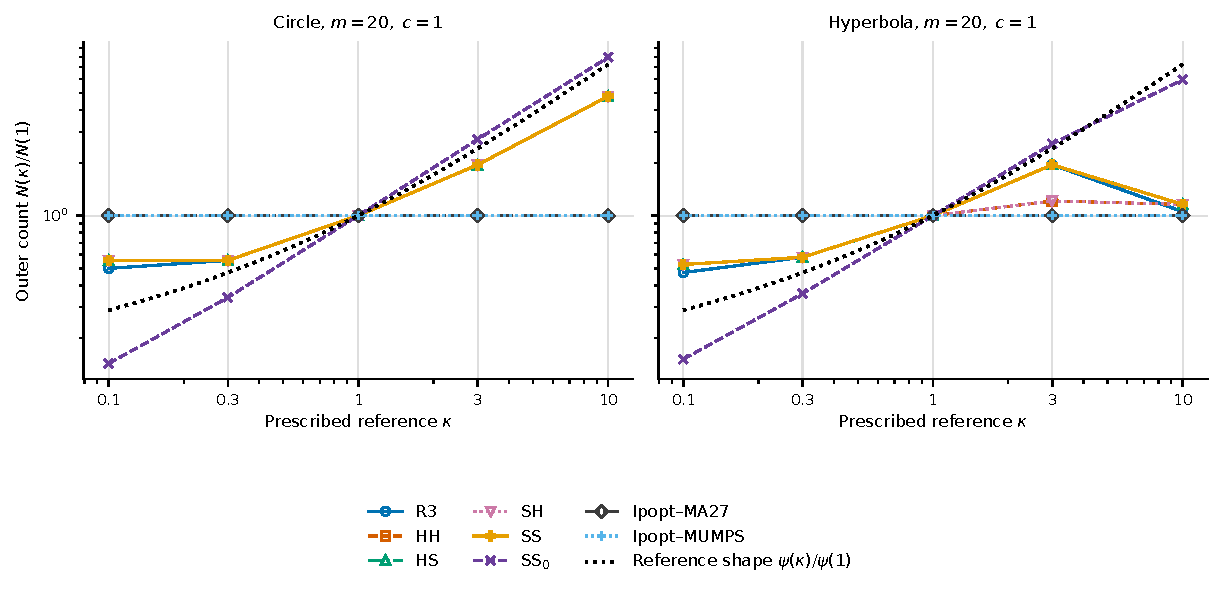
\includegraphics[width=\linewidth]{fig_controlled_reference_shape.pdf}
\caption{Normalized outer counts on the controlled designs with
$m=20$ and $c=1$. Every observed curve is divided by its count at
the design value $\kappa=1$; the black curve is
$\psi(\kappa)/\psi(1)$, a reference shape for a fixed asymptotic
error reduction. Five distinct problems determine each observed curve.
The prescribed reference $\kappa$ is not an estimate of the correction
retained by each configuration.}
\label{fig:controlled-reference-shape}
\end{figure}

\FloatBarrier

\section{Complete benchmark results}\label{app:complete-results}
Table~\ref{tab:global-classifications} reports success and failure counts
on the complete collection. All coverage percentages use the planned
instance count.
\begin{table}[!htbp]
\centering\small
\caption{Original-KKT outcomes over 4,078 planned instances per
configuration. Each cell lists success/failure counts.}
\label{tab:global-classifications}

% Local input expanded: classification_totals_backends.tex
\begin{tabular}{@{}llrrrrr@{}}
\toprule
Policy & Linear solver & I & M & E & Q & All \\
\midrule
R3 & MA27 & 996/41 & 663/134 & 1324/380 & 537/3 & 3520/558 \\
HH & MA27 & 888/149 & 661/136 & 1492/212 & 536/4 & 3577/501 \\
HS & MA27 & 889/148 & 622/175 & 1492/212 & 536/4 & 3539/539 \\
SH & MA27 & 887/150 & 661/136 & 1492/212 & 536/4 & 3576/502 \\
SS & MA27 & 889/148 & 660/137 & 1492/212 & 536/4 & 3577/501 \\
$SS_0$ & MA27 & 682/355 & 51/746 & 1248/456 & 519/21 & 2500/1578 \\
R3 & MUMPS & 1026/11 & 660/137 & 1314/390 & 540/0 & 3540/538 \\
HH & MUMPS & 895/142 & 660/137 & 1527/177 & 537/3 & 3619/459 \\
HS & MUMPS & 891/146 & 621/176 & 1527/177 & 537/3 & 3576/502 \\
SH & MUMPS & 894/143 & 660/137 & 1527/177 & 536/4 & 3617/461 \\
SS & MUMPS & 891/146 & 659/138 & 1527/177 & 536/4 & 3613/465 \\
$SS_0$ & MUMPS & 685/352 & 52/745 & 1249/455 & 519/21 & 2505/1573 \\
Ipopt monotone & MA27 & 1008/29 & 438/359 & 1485/219 & 534/6 & 3465/613 \\
Ipopt monotone & MUMPS & 1007/30 & 423/374 & 1153/551 & 536/4 & 3119/959 \\
Ipopt adaptive & MA27 & 989/48 & 336/461 & 1373/331 & 537/3 & 3235/843 \\
Ipopt adaptive & MUMPS & 989/48 & 310/487 & 1336/368 & 537/3 & 3172/906 \\
\bottomrule
\end{tabular}


\end{table}

\begin{scaledtable}[!htbp]
\centering\small
\caption{Strict certificates by benchmark collection, native MA27 and both certificate-matched Ipopt strategies with MA27. Structural
regimes remain the primary comparison; these rows localize the
contributions of individual collections. $^\dagger$Acquisition references
remain incomplete for three pose-graph and four UR10/Schunk instances within
the marked collections.}
\label{tab:mega-families}
\resizebox{\linewidth}{!}{
% Local input expanded: dataset_coverage_native_ma27.tex
\begin{tabular}{@{}lrrrrrrrrr@{}}
\toprule
Collection & $N$ & R3 & HH & HS & SH & SS & $SS_0$ & Ipopt mono & Ipopt adapt \\
\midrule
CBLIB & 6 & 4 & 4 & 4 & 4 & 4 & 0 & 5 & 5 \\
COPS camshape & 104 & 104 & 100 & 99 & 100 & 99 & 8 & 104 & 104 \\
COPS minimal surface & 100 & 100 & 23 & 28 & 23 & 28 & 0 & 96 & 77 \\
CUTEst & 136 & 127 & 122 & 120 & 121 & 120 & 96 & 109 & 113 \\
GasLib134 & 1208 & 1208 & 1208 & 1208 & 1208 & 1208 & 1208 & 1185 & 1185 \\
Other GasLib & 2 & 2 & 2 & 2 & 2 & 2 & 2 & 2 & 2 \\
IJOC partition QCQP & 150 & 150 & 150 & 150 & 150 & 150 & 150 & 150 & 150 \\
MINLPLib & 12 & 10 & 12 & 12 & 12 & 12 & 0 & 12 & 11 \\
Boundary control & 100 & 71 & 62 & 62 & 62 & 62 & 44 & 100 & 100 \\
Distributed control & 100 & 95 & 81 & 81 & 81 & 81 & 76 & 84 & 83 \\
PGLib & 198 & 196 & 196 & 196 & 196 & 196 & 7 & 140 & 193 \\
QPLIB & 49 & 47 & 47 & 47 & 47 & 47 & 35 & 48 & 48 \\
Array safety & 3 & 0 & 0 & 0 & 0 & 0 & 0 & 0 & 0 \\
ASU radio-beamforming & 503 & 375 & 375 & 337 & 375 & 375 & 0 & 212 & 58 \\
Controlled curvature & 60 & 60 & 60 & 60 & 60 & 60 & 60 & 60 & 60 \\
Coupled gas/power & 3 & 3 & 3 & 3 & 3 & 3 & 1 & 2 & 3 \\
Gas transport & 1 & 1 & 0 & 0 & 0 & 0 & 0 & 1 & 1 \\
Particle potential & 4 & 4 & 4 & 4 & 4 & 4 & 1 & 4 & 4 \\
Multicast beamforming & 129 & 129 & 128 & 127 & 128 & 127 & 72 & 129 & 129 \\
Path smoothing & 90 & 90 & 90 & 90 & 90 & 90 & 80 & 90 & 90 \\
Disk packing & 60 & 60 & 60 & 60 & 60 & 60 & 60 & 60 & 60 \\
MINLPLib pooling & 73 & 58 & 53 & 52 & 53 & 52 & 2 & 33 & 24 \\
Luedtke pooling & 360 & 9 & 177 & 177 & 177 & 177 & 0 & 228 & 122 \\
Reduced pooling & 2 & 0 & 0 & 0 & 0 & 0 & 0 & 0 & 1 \\
2D pose graph$^\dagger$ & 3 & 3 & 3 & 3 & 3 & 3 & 0 & 3 & 3 \\
Robot arm$^\dagger$ & 504 & 504 & 504 & 504 & 504 & 504 & 504 & 500 & 500 \\
Two ellipsoids & 90 & 90 & 90 & 90 & 90 & 90 & 90 & 90 & 90 \\
Water networks & 28 & 20 & 23 & 23 & 23 & 23 & 4 & 18 & 19 \\
\bottomrule
\end{tabular}

}
\end{scaledtable}


\begin{scaledtable}[!htbp]
\centering\small
\caption{Strict certificates by collection, native MUMPS and both certificate-matched Ipopt strategies with MUMPS. Structural regimes remain primary; these rows locate collection contributions. The acquisition-reference marks have the same meaning as in Table~\ref{tab:mega-families}.}
\label{tab:mega-families-native-mumps}
\resizebox{\linewidth}{!}{
% Local input expanded: dataset_coverage_native_mumps.tex
\begin{tabular}{@{}lrrrrrrrrr@{}}
\toprule
Collection & $N$ & R3 & HH & HS & SH & SS & $SS_0$ & Ipopt mono & Ipopt adapt \\
\midrule
CBLIB & 6 & 5 & 5 & 3 & 5 & 3 & 0 & 4 & 4 \\
COPS camshape & 104 & 104 & 102 & 99 & 102 & 99 & 8 & 104 & 104 \\
COPS minimal surface & 100 & 100 & 23 & 27 & 23 & 27 & 0 & 96 & 79 \\
CUTEst & 136 & 132 & 125 & 123 & 123 & 122 & 97 & 114 & 115 \\
GasLib134 & 1208 & 1208 & 1207 & 1207 & 1207 & 1207 & 1208 & 833 & 988 \\
Other GasLib & 2 & 2 & 2 & 2 & 2 & 2 & 2 & 2 & 2 \\
IJOC partition QCQP & 150 & 150 & 150 & 150 & 150 & 150 & 150 & 150 & 150 \\
MINLPLib & 12 & 10 & 12 & 12 & 12 & 12 & 0 & 12 & 10 \\
Boundary control & 100 & 100 & 66 & 66 & 66 & 66 & 46 & 100 & 100 \\
Distributed control & 100 & 95 & 81 & 81 & 81 & 81 & 76 & 84 & 83 \\
PGLib & 198 & 195 & 196 & 196 & 196 & 196 & 7 & 123 & 167 \\
QPLIB & 49 & 47 & 47 & 47 & 47 & 47 & 35 & 48 & 48 \\
Array safety & 3 & 0 & 0 & 0 & 0 & 0 & 0 & 0 & 0 \\
ASU radio-beamforming & 503 & 375 & 375 & 337 & 375 & 375 & 0 & 214 & 55 \\
Controlled curvature & 60 & 60 & 60 & 60 & 60 & 60 & 60 & 60 & 60 \\
Coupled gas/power & 3 & 3 & 3 & 3 & 3 & 3 & 2 & 2 & 2 \\
Gas transport & 1 & 1 & 0 & 0 & 0 & 0 & 0 & 1 & 1 \\
Particle potential & 4 & 4 & 4 & 4 & 4 & 4 & 1 & 4 & 4 \\
Multicast beamforming & 129 & 129 & 128 & 127 & 128 & 127 & 72 & 128 & 129 \\
Path smoothing & 90 & 90 & 90 & 90 & 90 & 90 & 80 & 90 & 90 \\
Disk packing & 60 & 60 & 60 & 60 & 60 & 60 & 60 & 60 & 60 \\
MINLPLib pooling & 73 & 51 & 56 & 55 & 56 & 55 & 2 & 34 & 22 \\
Luedtke pooling & 360 & 5 & 207 & 207 & 207 & 207 & 0 & 245 & 285 \\
Reduced pooling & 2 & 0 & 0 & 0 & 0 & 0 & 0 & 0 & 1 \\
2D pose graph$^\dagger$ & 3 & 3 & 3 & 3 & 3 & 3 & 0 & 3 & 3 \\
Robot arm$^\dagger$ & 504 & 503 & 503 & 503 & 503 & 503 & 504 & 500 & 500 \\
Two ellipsoids & 90 & 90 & 90 & 90 & 90 & 90 & 90 & 90 & 90 \\
Water networks & 28 & 18 & 24 & 24 & 24 & 24 & 5 & 18 & 20 \\
\bottomrule
\end{tabular}

}
\end{scaledtable}

\section{Matched timings across all regimes}\label{app:all-policy-comparisons}
The ordering of a pair fixes the numerator and denominator of its time
ratio. Every cell in Table~\ref{tab:mega-all-pairs} reports a median of
individual elapsed-process ratios and the corresponding common-certificate
sample size. A problem contributes only when both final points meet the
same original KKT threshold. These pair-specific cohorts complement the
joint performance profiles in Figure~\ref{fig:performance-profiles}.
\begin{scaledtable}[!htbp]
\centering\small
\caption{All 28 paired time comparisons among the six native MA27 policies and both certificate-matched Ipopt strategies with MA27. Values below one favor the
numerator; brackets give eligible sample sizes.}
\label{tab:mega-all-pairs}
\resizebox{\linewidth}{!}{
% Local input expanded: paired_all.tex
\begin{tabular}{@{}lrrrrr@{}}
\toprule
Numerator / denominator & I & M & E & Q & All \\
\midrule
R3 / HH & 0.192 [885] & 0.0986 [660] & 1 [1316] & 0.568 [536] & 0.61 [3397] \\
R3 / HS & 0.185 [886] & 0.0737 [621] & 0.998 [1316] & 0.529 [536] & 0.59 [3359] \\
R3 / SH & 0.246 [884] & 0.1 [660] & 0.999 [1316] & 0.531 [536] & 0.595 [3396] \\
R3 / SS & 0.256 [886] & 0.0877 [659] & 1 [1316] & 0.569 [536] & 0.617 [3397] \\
R3 / $SS_0$ & 0.522 [682] & 0.58 [51] & 0.999 [1248] & 0.997 [519] & 0.959 [2500] \\
R3 / Ipopt mono & 1.44 [977] & 1.04 [438] & 1.5 [1258] & 0.905 [532] & 1.41 [3205] \\
R3 / Ipopt adapt & 1.43 [957] & 1.43 [335] & 1.5 [1247] & 0.901 [534] & 1.43 [3073] \\
HH / HS & 1 [882] & 0.805 [622] & 1 [1492] & 0.987 [536] & 0.997 [3532] \\
HH / SH & 0.994 [887] & 0.999 [661] & 1 [1492] & 0.988 [536] & 0.999 [3576] \\
HH / SS & 1.06 [882] & 0.994 [660] & 1 [1492] & 1.02 [536] & 1.01 [3570] \\
HH / $SS_0$ & 2.37 [679] & 1.23 [51] & 1 [1248] & 1.74 [519] & 1.11 [2497] \\
HH / Ipopt mono & 11 [884] & 5.3 [436] & 1.51 [1371] & 1.57 [532] & 1.8 [3223] \\
HH / Ipopt adapt & 10.4 [877] & 4.01 [334] & 1.51 [1296] & 1.59 [534] & 1.7 [3041] \\
HS / SH & 0.995 [882] & 1.22 [622] & 1 [1492] & 1.01 [536] & 1.01 [3532] \\
HS / SS & 1.05 [889] & 1.1 [622] & 1 [1492] & 1.05 [536] & 1.03 [3539] \\
HS / $SS_0$ & 2.27 [679] & 1.35 [51] & 1.01 [1248] & 1.85 [519] & 1.12 [2497] \\
HS / Ipopt mono & 11.1 [885] & 7.57 [412] & 1.51 [1371] & 1.72 [532] & 1.86 [3200] \\
HS / Ipopt adapt & 10.6 [878] & 4.41 [329] & 1.5 [1296] & 1.69 [534] & 1.75 [3037] \\
SH / SS & 1.04 [882] & 0.994 [660] & 1 [1492] & 1.03 [536] & 1.01 [3570] \\
SH / $SS_0$ & 2.27 [679] & 1.23 [51] & 1 [1248] & 1.83 [519] & 1.1 [2497] \\
SH / Ipopt mono & 7.57 [883] & 5.33 [436] & 1.51 [1371] & 1.67 [532] & 1.85 [3222] \\
SH / Ipopt adapt & 7.25 [876] & 4.04 [334] & 1.51 [1296] & 1.66 [534] & 1.72 [3040] \\
SS / $SS_0$ & 1.88 [679] & 1.06 [51] & 1.01 [1248] & 1.72 [519] & 1.07 [2497] \\
SS / Ipopt mono & 6.87 [885] & 5.87 [435] & 1.51 [1371] & 1.57 [532] & 1.75 [3223] \\
SS / Ipopt adapt & 6.83 [878] & 4.28 [333] & 1.5 [1296] & 1.58 [534] & 1.68 [3041] \\
$SS_0$ / Ipopt mono & 2.81 [681] & 3.13 [47] & 1.5 [1215] & 0.903 [516] & 1.49 [2459] \\
$SS_0$ / Ipopt adapt & 2.74 [680] & 2.26 [47] & 1.5 [1216] & 0.892 [518] & 1.49 [2461] \\
Ipopt mono / Ipopt adapt & 0.999 [985] & 0.997 [261] & 0.999 [1318] & 1 [534] & 0.999 [3098] \\
\bottomrule
\end{tabular}

}
\end{scaledtable}

\FloatBarrier


\begin{scaledtable}[!htbp]
\centering\small
\caption{All 28 paired time comparisons among the six native MUMPS policies and both certificate-matched Ipopt strategies with MUMPS. Each ratio uses its own common-certificate cohort; values below one favor the first configuration.}
\label{tab:mega-all-pairs-native-mumps}
\resizebox{\linewidth}{!}{
% Local input expanded: paired_all_native_mumps.tex
\begin{tabular}{@{}lrrrrr@{}}
\toprule
Numerator / denominator & I & M & E & Q & All \\
\midrule
R3 / HH & 0.204 [893] & 0.112 [657] & 0.995 [1310] & 0.657 [537] & 0.649 [3397] \\
R3 / HS & 0.189 [890] & 0.0804 [618] & 0.988 [1310] & 0.656 [537] & 0.654 [3355] \\
R3 / SH & 0.26 [892] & 0.114 [657] & 0.981 [1310] & 0.654 [536] & 0.644 [3395] \\
R3 / SS & 0.272 [890] & 0.0963 [656] & 0.99 [1310] & 0.648 [536] & 0.642 [3392] \\
R3 / $SS_0$ & 0.432 [685] & 0.36 [51] & 0.994 [1249] & 0.924 [519] & 0.902 [2504] \\
R3 / Ipopt mono & 1.11 [1006] & 0.565 [421] & 1.34 [907] & 0.933 [536] & 1.09 [2870] \\
R3 / Ipopt adapt & 1.08 [987] & 0.656 [307] & 1.31 [1049] & 0.916 [537] & 1.08 [2880] \\
HH / HS & 1 [885] & 0.785 [621] & 0.997 [1527] & 0.997 [537] & 0.991 [3570] \\
HH / SH & 0.987 [894] & 0.998 [660] & 0.995 [1527] & 0.997 [536] & 0.995 [3617] \\
HH / SS & 1.05 [885] & 0.987 [659] & 0.998 [1527] & 0.998 [536] & 1 [3607] \\
HH / $SS_0$ & 2.04 [682] & 0.885 [50] & 0.993 [1248] & 1.38 [519] & 1.08 [2499] \\
HH / Ipopt mono & 7.23 [890] & 3.76 [420] & 1.49 [1058] & 1.39 [535] & 1.73 [2903] \\
HH / Ipopt adapt & 6.81 [884] & 2 [307] & 1.43 [1214] & 1.38 [536] & 1.61 [2941] \\
HS / SH & 0.996 [885] & 1.23 [621] & 0.999 [1527] & 1.01 [536] & 1.01 [3569] \\
HS / SS & 1.05 [891] & 1.07 [621] & 1 [1527] & 0.999 [536] & 1.02 [3575] \\
HS / $SS_0$ & 1.99 [682] & 1.02 [50] & 0.998 [1248] & 1.39 [519] & 1.1 [2499] \\
HS / Ipopt mono & 7.76 [888] & 5.89 [397] & 1.5 [1058] & 1.42 [535] & 1.73 [2878] \\
HS / Ipopt adapt & 7.41 [882] & 2.08 [302] & 1.43 [1214] & 1.41 [536] & 1.61 [2934] \\
SH / SS & 1.04 [885] & 0.997 [659] & 1 [1527] & 0.996 [536] & 1.01 [3607] \\
SH / $SS_0$ & 1.97 [682] & 0.948 [50] & 0.999 [1248] & 1.38 [519] & 1.1 [2499] \\
SH / Ipopt mono & 3.87 [889] & 3.86 [420] & 1.49 [1058] & 1.43 [534] & 1.72 [2901] \\
SH / Ipopt adapt & 4.02 [883] & 2.01 [307] & 1.42 [1214] & 1.4 [535] & 1.59 [2939] \\
SS / $SS_0$ & 1.71 [682] & 0.971 [50] & 0.992 [1248] & 1.4 [519] & 1.08 [2499] \\
SS / Ipopt mono & 3.81 [888] & 4.13 [419] & 1.48 [1058] & 1.43 [534] & 1.73 [2899] \\
SS / Ipopt adapt & 3.81 [882] & 2.02 [306] & 1.4 [1214] & 1.41 [535] & 1.6 [2937] \\
$SS_0$ / Ipopt mono & 2.87 [683] & 2.8 [48] & 1.4 [865] & 1.03 [517] & 1.4 [2113] \\
$SS_0$ / Ipopt adapt & 2.8 [683] & 2.99 [48] & 1.33 [1019] & 1.02 [518] & 1.35 [2268] \\
Ipopt mono / Ipopt adapt & 0.995 [985] & 0.997 [235] & 0.999 [969] & 0.999 [535] & 0.998 [2724] \\
\bottomrule
\end{tabular}

}
\end{scaledtable}

\begin{figure}[!htbp]
\centering
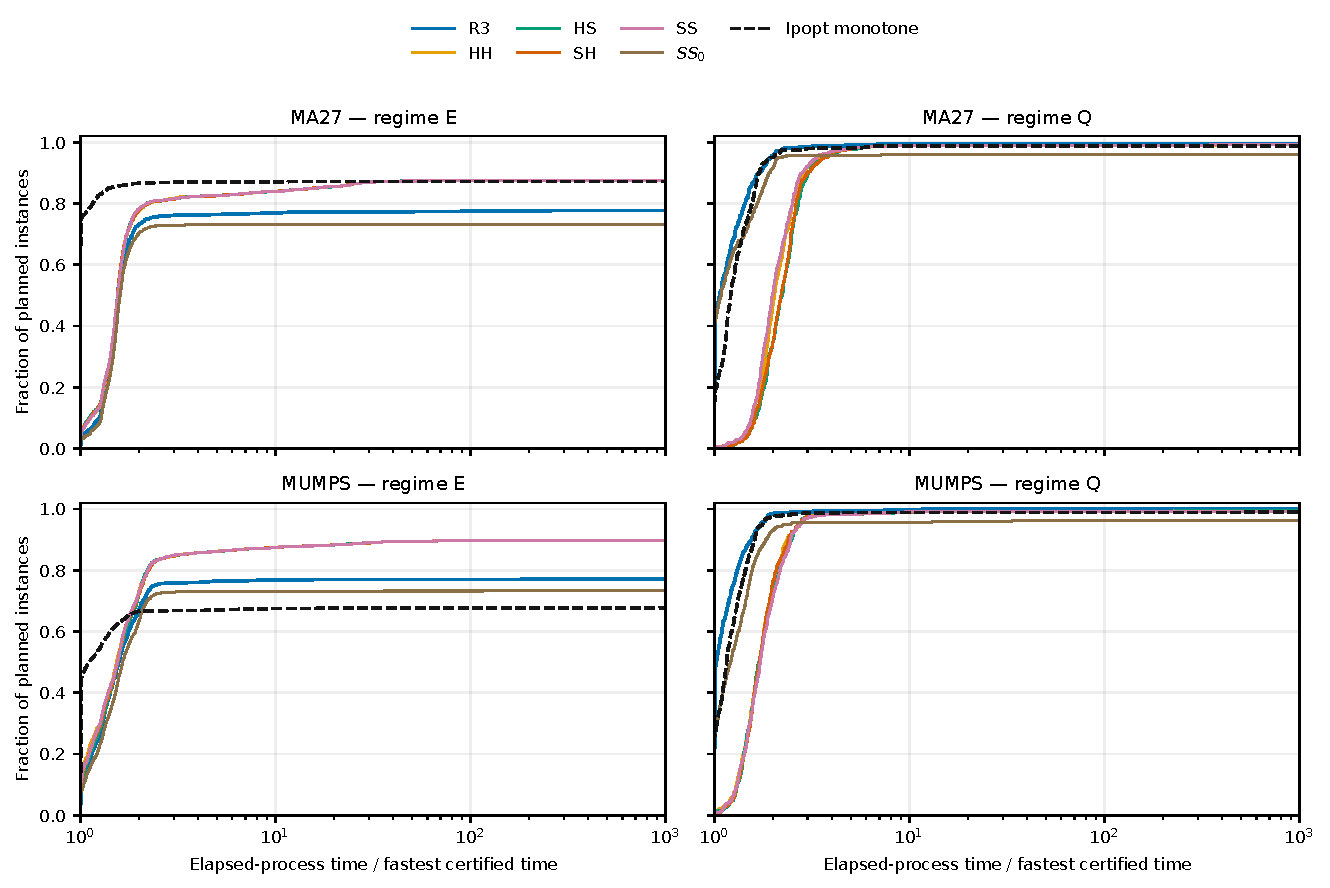
\includegraphics[width=\linewidth]{fig_aligned_equality_performance_profiles.pdf}
\caption{Elapsed-process performance profiles in E and Q. Rows indicate
the linear solver; each panel compares the six native policies with monotone Ipopt at certificate-matched stopping targets.
Every planned instance remains in its denominator and failures receive
infinite ratios. These profiles have no objective-equivalence restriction.}
\label{fig:equality-performance-profiles}
\end{figure}


\FloatBarrier
\section{Direct H/S objective comparisons}\label{app:quartet-direct-objectives}
Table~\ref{tab:quartet-direct} gives the pair-specific common-cohort
comparisons, including their quartiles, for both linear solvers.

\begin{table}[t]
\centering\footnotesize
\setlength{\tabcolsep}{3pt}
\caption{Direct ASU objectives within the H/S quartet on pair-specific
common certificates. Gaps are percent values; L/E/H counts lower,
equivalent and higher objectives for the first policy at $10^{-3}$.
SS comparisons include different implied-bound preprocessing.}
\label{tab:quartet-direct}

% Local input expanded: quartet_ASU_direct_main.tex
\begin{tabular}{@{}llrcc@{}}
\toprule
Linear solver & Direct pair & $N$ & Median $[Q_1,Q_3]$ (\%) & L/E/H\\
\midrule
MA27 & SS/SH & 375 & 17.82 [11.50,24.65] & 1/3/371\\
MA27 & SS/HS & 337 & 16.10 [10.50,22.16] & 2/0/335\\
MA27 & SS/HH & 375 & 17.82 [11.50,24.65] & 1/3/371\\
MA27 & HH/SH & 375 & 0.00 [0.00,0.00] & 0/375/0\\
\addlinespace
MUMPS & SS/SH & 375 & 17.82 [11.50,24.65] & 1/4/370\\
MUMPS & SS/HS & 337 & 16.10 [10.50,22.16] & 2/1/334\\
MUMPS & SS/HH & 375 & 17.82 [11.50,24.65] & 1/4/370\\
MUMPS & HH/SH & 375 & 0.00 [0.00,0.00] & 0/375/0\\
\bottomrule
\end{tabular}


\end{table}


For each linear solver, the four configurations use the same 4,078
instances, with matching original inputs and raw and internally stored starts.
The analysis uses the archived strict classifications and their exported
primal, dual and complementarity residuals, all finite and at most
$10^{-6}$. These exports contain no full solution vectors.

For a pair $(A,B)$ the signed objective gap is
$\delta_f(A,B)=(f_A-f_B)/\max\{1,|f_A|,|f_B|\}$. Positive values mean
that $B$ attains a lower minimization objective. The pair-specific cohort
contains the instances certified by those two policies. The four-way
cohort contains the instances certified by HH, HS, SH and SS jointly.
Both comparisons use the same coefficients and raw initial point.
Quantiles use the type-7 empirical definition on the entire paired cohort.

On ASU, HH, SH and SS each certify 375 of the 503 planned instances;
HS certifies 337. All 337 HS certificates belong to the joint four-way
cohort. The pair-specific $SS/SH$ and $SS/HH$ cohorts therefore contain
375 cases, whereas the four-way comparisons use 337. On this joint
cohort, the median gaps are $16.0970\%$ for $SS/SH$ and $SS/HH$, and
$16.1022\%$ for $SS/HS$, with either linear solver. Pair-specific
$SS/SH$ and $SS/HH$ medians are $17.8232\%$. The different certified cohorts account for the difference between these
summaries.

\begin{table}[t]
\centering\small
\caption{Direct ASU H/S comparisons on the 337 common certificates of all
four policies. Gaps are percent values; the last column counts exactly
equal exported objectives.}
\label{tab:quartet-four-common}

% Local input expanded: quartet_ASU_common_SI.tex
\begin{tabular}{@{}llrcr@{}}
\toprule
Linear solver & Pair & $N$ & Median $[Q_1,Q_3]$ (\%) & Exact equal\\
\midrule
MA27 & SS/SH & 337 & 16.10 [10.88,22.61] & 0\\
MA27 & SS/HS & 337 & 16.10 [10.50,22.16] & 0\\
MA27 & SS/HH & 337 & 16.10 [10.88,22.61] & 0\\
MA27 & HH/SH & 337 & 0.00 [0.00,0.00] & 336\\
MA27 & HH/HS & 337 & 0.00 [-0.02,0.00] & 0\\
MA27 & SH/HS & 337 & 0.00 [-0.02,0.00] & 0\\
\addlinespace
MUMPS & SS/SH & 337 & 16.10 [10.88,22.61] & 0\\
MUMPS & SS/HS & 337 & 16.10 [10.50,22.16] & 0\\
MUMPS & SS/HH & 337 & 16.10 [10.88,22.61] & 0\\
MUMPS & HH/SH & 337 & 0.00 [0.00,0.00] & 337\\
MUMPS & HH/HS & 337 & 0.00 [-0.02,0.00] & 0\\
MUMPS & SH/HS & 337 & 0.00 [-0.02,0.00] & 0\\
\bottomrule
\end{tabular}


\end{table}

To examine additivity without mixing normalizations, define for each
jointly certified instance
\[
 D_i=\max\{1,|f_{HH,i}|,|f_{HS,i}|,|f_{SH,i}|,|f_{SS,i}|\},\qquad
 I_i=\frac{f_{HH,i}-f_{HS,i}-f_{SH,i}+f_{SS,i}}{D_i}.
\]
The scale $D_i$ is shared by all four policies on that instance. A
positive $I_i$ means that the joint reduction from SS to HH is smaller
than the sum of the two separate reductions from SS to HS and SH.
On the 337 ASU instances, the median of $I_i$ is $16.1022\%$, with
quartiles $10.5021\%$ and $22.1601\%$, for both linear solvers. This
is an arithmetic contrast of attained objectives; it is not an isolated
causal estimate for curvature refinement. In particular, the source
audit documents different treatment of implied bounds between SS and
the other three policies.

HH and SH have equal exported objectives on all 375 common MUMPS
certificates. With MA27, 374 are exactly equal and one relative gap is
$2.1136\times10^{-13}$. All pairs are equivalent at thresholds $10^{-3}$
and $10^{-2}$. These comparisons concern exported objective values. The available data
contain no full primal vectors, iteration histories or record of the active
correction matrices.

Outside ASU, median $SS/SH$, $SS/HS$ and $SS/HH$ objective gaps are zero
with both linear solvers. At threshold $10^{-3}$, all 285 MA27 $SS/HS$
pairs are equivalent, and 284 of 285 $SS/SH$ or $SS/HH$ pairs are
equivalent; the remaining pair favors the latter policy. The MUMPS
counts are 284 of 284 for $SS/HS$ and 283 of 284 for $SS/SH$ or $SS/HH$.
Every outside-ASU pair is equivalent at $10^{-2}$ in these comparisons.
Thus the substantial direct objective differences are concentrated in
the constructed ASU collection and in the available common-certificate
cohorts; no distance to a globally optimal value follows from them.

\subsection{Comparisons with common presolve and safeguards}
The source audit distinguishes the HS/HH and SH/HH comparisons from the
SS comparisons. In HS/HH the objective policy is hybrid in both settings;
in SH/HH the inequality policy is hybrid in both settings. These two
comparisons share the implied-bound treatment, acceptance rules and
safeguards. Their recorded settings specify identical budgets of 7,200
seconds, 5,000 outer iterations and 600 shared restoration iterations,
with one numerical thread and original residual thresholds $10^{-6}$.

\begin{table}[t]
\centering\small
\caption{Paired strict-certificate counts for the two H/S comparisons with
common preprocessing. The categories partition all planned instances;
only the stated correction policy changes.}
\label{tab:quartet-clean-edge-coverage}

% Local input expanded: quartet_clean_edge_coverage_SI.tex
\begin{tabular}{@{}lllrrrrr@{}}
\toprule
Linear solver & $A/B$ & Scope & $N$ & Both & $A$ only & $B$ only & Neither\\
\midrule
MA27 & HS/HH & ASU & 503 & 337 & 0 & 38 & 128\\
MA27 & HS/HH & M & 797 & 622 & 0 & 39 & 136\\
MA27 & HS/HH & I & 1037 & 882 & 7 & 6 & 142\\
MA27 & SH/HH & ASU & 503 & 375 & 0 & 0 & 128\\
MA27 & SH/HH & M & 797 & 661 & 0 & 0 & 136\\
MA27 & SH/HH & I & 1037 & 887 & 0 & 1 & 149\\
MUMPS & HS/HH & ASU & 503 & 337 & 0 & 38 & 128\\
MUMPS & HS/HH & M & 797 & 621 & 0 & 39 & 137\\
MUMPS & HS/HH & I & 1037 & 885 & 6 & 10 & 136\\
MUMPS & SH/HH & ASU & 503 & 375 & 0 & 0 & 128\\
MUMPS & SH/HH & M & 797 & 660 & 0 & 0 & 137\\
MUMPS & SH/HH & I & 1037 & 894 & 0 & 1 & 142\\
\bottomrule
\end{tabular}


\end{table}

The HS/HH comparison has 38 HH-only ASU certificates and no HS-only certificate
with each linear solver. The additional mixed-regime certificate outside
ASU belongs to a pooling model. In I, the MA27 comparison has six HH-only and
seven HS-only certificates, while MUMPS has ten and six. Across I and M
jointly, the corresponding HH-only/HS-only counts are 45/7 and 49/6.
The net difference is therefore 38 or 43, strongly concentrated in ASU.
SH/HH has no mixed-regime discordance and only one HH-only certificate
in I, on a CUTEst case, with each linear solver.

On the 337 shared ASU HS/HH certificates, the median signed objective
gap is approximately $-6.7\times10^{-11}$. With $A=HS$ and $B=HH$,
threshold $10^{-3}$ gives 65 lower, 198 equivalent and 74 higher
objectives; threshold $10^{-2}$ gives 20, 296 and 21. These counts hold
for both linear solvers. The additional HH certificates are accompanied by a near-zero median
paired objective gap on the shared ASU cohort. This comparison holds
implied-bound preprocessing fixed; the SS-relative contrasts also include
its change.


\subsection{Signed medians and the implied-bound hypothesis}\label{app:asu-bound-hypothesis}
Absolute gaps and threshold counts complement the signed median in
describing objective differences.
On the 375 ASU R3/SS
certificates, the median absolute symmetric gap is $0.7878\%$ for either
backend. At $10^{-3}$, MA27 gives 78 lower, 126 equivalent and 171 higher
R3 objectives; MUMPS gives 77, 127 and 171. At $10^{-2}$ the counts are
47, 199 and 129 for both. No exported R3/SS objective is exactly equal;
the signed gaps range from $-9.74\%$ to $16.91\%$.
The HS/HH median is also almost zero, but 139/337 pairs exceed $0.1\%$
in absolute gap and 41/337 exceed $1\%$. In contrast, the SH/HH objectives
agree to the precision reported above. Table~\ref{tab:asu-objective-dispersion}
reports signed and absolute summaries on the pair-specific cohorts.

\begin{scaledtable}[!htbp]
\centering\footnotesize
\caption{ASU objective dispersion on common original certificates.
Signed and absolute medians are in percent. L/E/H refers
to the first policy in each pair; the two thresholds are dimensionless.}
\label{tab:asu-objective-dispersion}
\resizebox{\linewidth}{!}{
% Local input expanded: asu_distribution_compact_R13.tex
\begin{tabular}{@{}llrcccc@{}}
\toprule
Solver & $A/B$ & $N$ & Med. $\delta_f$ & Med. $|\delta_f|$ & L/E/H $10^{-3}$ & L/E/H $10^{-2}$\\
\midrule
MA27 & R3/SS & 375 & 0.00 & 0.788 & 78/126/171 & 47/199/129\\
MA27 & SS/HH & 375 & 17.823 & 17.823 & 1/3/371 & 0/11/364\\
MA27 & HS/HH & 337 & 0.00 & 0.000159 & 65/198/74 & 20/296/21\\
MA27 & SH/HH & 375 & 0.00 & 0.00 & 0/375/0 & 0/375/0\\
\addlinespace
MUMPS & R3/SS & 375 & 0.00 & 0.788 & 77/127/171 & 47/199/129\\
MUMPS & SS/HH & 375 & 17.823 & 17.823 & 1/4/370 & 0/11/364\\
MUMPS & HS/HH & 337 & 0.00 & 0.000159 & 65/198/74 & 20/296/21\\
MUMPS & SH/HH & 375 & 0.00 & 0.00 & 0/375/0 & 0/375/0\\
\bottomrule
\end{tabular}

}
\end{scaledtable}

The presolve rule enables removal of bound sides proved by a quadratic
equality for HH, HS and SH, and excludes R3 and SS. On the available
ASU MA27 observations, R3 removes zero sides on all 503 cases, with
unchanged dimensions; the corresponding HH/HS/SH counts are stated in
the article. The same rule occurs in both archived backend sources.
An equality-radial implication proves redundancy on the original feasible
set; it does not by itself establish whether that bound is strictly
inactive or active at every feasible point. The observed input metadata
and counters do not reconstruct central paths.

For an affine bound $a^Tx\leq b$ with positive slack $t(x)=b-a^Tx$, its
logarithmic barrier contribution and derivatives are
\[
 -\mu\log t(x),\qquad
 \frac{\mu a}{t(x)},\qquad
 \frac{\mu aa^T}{t(x)^2}.
\]
Deleting a redundant bound removes these terms at positive $\mu$, although
the original feasible set and objective are preserved. This gives a
mechanism for representation-dependent trajectories. Redundant LP
representations have strongly different central paths
\citep{DezaNematollahiTerlaky2008,NematollahiTerlaky2008Touching}; those
constructions converge to the same optimum. Their geometric path curvature
is distinct from the component excess $\kappa$ studied here. The LP results
do not prove that removing bounds selects a different stationary point
in these nonconvex QCQPs, nor that it causes the observed ASU objective gaps.

The following controlled experiment isolates this preprocessing rule.
It is distinct from Section~\ref{app:controlled-refinement}, which varies
refinement and globalization while retaining quadratically implied bounds.

\subsection{Controlled implied-bound removal}\label{supp:asu-bounds}
Each of the 503 ASU problems is solved with R3, SS and HH, with
quadratically implied bounds retained or removed, using MA27 or MUMPS:
6,036 observations.
A common implementation changes only the rule for bounds proved redundant
by a quadratic equality; inputs, raw starts, policy settings and budgets
are fixed within each pair. Other presolve rules remain fixed. Removal
deletes 128 bound sides in 501 cases and 64 in two. The complete original
bounds remain in the independent KKT audit. Before production,
144 qualification executions compare the original and modified versions on
72 pairs of configurations; final points, work, presolve and audits agree.
The 144 pilot observations are included in the 6,036 campaign observations,
not added a second time. These controls isolate the tested change in this
implementation; equivalence to the historical MUMPS executable is not claimed.

There are 4,285 strict certificates, 1,729 nonstrict final points and 22
administratively indeterminate observations lacking the complete resource
and audit records after controller interruption. The last category is
neither a numerical failure nor a reconstructed certificate. Recorded
nonstrict terminations comprise 1,493 line-search failures, 200 outer-cycle
limits and 36 inner failures. Removal adds no strict certificate. R3 loses
63 with each backend, all at the 5,000-cycle limit. SS loses 40 or 41:
37 cycle limits and three or four indeterminate observations. HH retains
the same 374 certified cases. All 503 cases remain in coverage denominators.

Table~\ref{tab:asu-bounds-pairs} supplements the article's comparison on
instances certified by all six configurations with pair-specific common
certificates. Define
\[
 g_b=\frac{f_{\rm keep}-f_{\rm remove}}
 {\max\{1,|f_{\rm keep}|,|f_{\rm remove}|\}}.
\]
Positive $g_b$ favours removal. These are normalized gaps, not uniformly
ordinary relative decreases, since some objective magnitudes are below one.
The sets certified by all six configurations contain 305 MA27 and 304 MUMPS cases, with
median $g_b$ between 0.157 and 0.162 across policies. Their restriction
avoids comparing different certified populations across policies; neither
cohort describes objectives on noncertified runs. The median paired objective gaps favor removal on the common cohort.
Over the full cohort, R3 and SS obtain fewer certificates after removal.
The ASU observations were recorded under concurrent execution.

\begin{table}[!htbp]
\centering\small\setlength{\tabcolsep}{4pt}
\caption{Controlled bound removal on pair-specific common certificates.
L/E/H compares the removed-bound objective with the retained-bound
objective at normalized tolerance $10^{-3}$. Gap values are $100g_b$.
Coverage and the comparison shared by all six configurations are reported
in the article.}
\label{tab:asu-bounds-pairs}
\begin{tabular}{@{}llrrr@{}}
\toprule
Backend & Policy & Common & Median gap [Q$_1$,Q$_3$] (\%) & L/E/H\\
\midrule
MA27 & R3 & 312 & 16.76 [9.91,22.17] & 309/2/1\\
MA27 & SS & 334 & 16.06 [10.47,22.08] & 332/0/2\\
MA27 & HH & 374 & 18.00 [12.23,24.91] & 369/2/3\\
MUMPS & R3 & 312 & 16.76 [9.91,22.17] & 309/2/1\\
MUMPS & SS & 333 & 16.02 [10.46,22.10] & 330/1/2\\
MUMPS & HH & 374 & 18.00 [12.23,24.91] & 369/2/3\\
\bottomrule
\end{tabular}
\end{table}
\FloatBarrier

\section{Persistent reuse of a fixed correction}\label{supp:persistence}
This ablation measures the construction cost saved by reusing the same
deterministic R3 correction. Reuse constructs it when a model is initialized; rebuild reconstructs it
at every model update, including updates at an unchanged iterate. The resulting corrections, other stored solver data,
globalization and factorization rules are unchanged. The comparison measures
construction cost with the same regularization matrices; it does not vary
their geometry or adaptive refinement.

Twelve cases (six I and six M) are selected by seeded, size-stratified
sampling among historical strict successes with both backends and process
times above one second: six PGLib, two multicast, two distributed-control,
one minimal-surface and QPLIB~3312. Selection does not use the new timing results. For each of the 24 case/backend pairs, the original, reuse and rebuild
versions give 72 qualification executions in total. Their numerical histories, recorded solver states and original
audit values agree exactly; there are 13,717 log records per mode. Final
points and work records agree across all six timed executions of each pair.
Qualification counters total 25 correction preparations under reuse and
4,638 under rebuild. Corrections are nonzero in 22 pairs; QPLIB~3312 under
both backends supplies a zero-correction control.

Timed runs use three repetitions per mode: 144 executions, all
strictly certified. Each starts a fresh, single-thread process on core 0,
sequentially, with balanced and reversed mode ordering. Each attempt follows
ten seconds of low CPU activity. CPU usage of other processes and of all
online cores is monitored throughout each solve. Four attempts affected by
other CPU activity are retained and repeated under the prespecified rule;
all four already had strict certificates. A completed numerical failure
without such interference would be retained. Process time includes
loading, startup and shutdown, but excludes the independent audit and
the waiting period. Detailed qualification logs are disabled during timing. This CPU
check does not exclude I/O or memory contention.

Each pair's time ratio divides the three-run reuse median by the three-run
rebuild median. Across the 12 pairs per backend, the median ratio is
0.849 [0.789,0.878] under MA27 and 0.853 [0.813,0.876] under MUMPS
[quartiles]; reuse is faster in all 24 pairs. The largest within-mode
three-run range divided by its median is 1.65\% for reuse and 2.67\% for
rebuild. Family effects in Table~\ref{tab:persistence-families} differ
substantially. The two multicast cases give speedups of 36.2--37.5,
whereas the zero-correction control changes by approximately one percent
or less. The reported reductions measure avoided reconstruction work on these
selected instances, with unchanged numerical results.

\begin{table}[!htbp]
\centering\small
\caption{Median process-time reduction $100(1-t_{\rm reuse}/t_{\rm rebuild})$
across cases in each family. Each pair ratio uses its three-run medians.}
\label{tab:persistence-families}
\begin{tabular}{@{}lrrr@{}}
\toprule
Family & Cases & MA27 (\%) & MUMPS (\%)\\
\midrule
PGLib & 6 & 15.07 & 14.68\\
Multicast & 2 & 97.30 & 97.27\\
Distributed control & 2 & 6.88 & 7.24\\
Minimal surface & 1 & 33.64 & 25.11\\
QPLIB 3312 (zero correction) & 1 & 1.01 & 0.56\\
\bottomrule
\end{tabular}
\end{table}
For both ablations, supplied scalar results agree with independent audits
and input and start hashes. The exports omit full
solution vectors, so no fresh residual evaluation is claimed.
\FloatBarrier

\section{Published reference solutions}\label{app:published-reference-values}
We compare original-certified objectives with published reference-point
values on 49 QPLIB and four MINLPLib facility-location problems in regime I.
The QPLIB values in the official solution list agree with those retained
at corpus acquisition; they are marked as best known, rather than proved
optimal. Three source problems maximize their objective, and their
reference values are multiplied by $-1$ to match the fixed minimization
problem. The archived conversion records preserve the continuous model,
bounds and objective, without integer relaxation. In particular, the
QPLIB lower-triangular quadratic convention requires halving an
off-diagonal entry when forming a symmetric Hessian. The MINLPLib
facility models use the recorded direct public continuous formulation,
with matching file hashes and archived independent checks of the model
conversion. These records establish the scope of the comparison; no new
model conversion or optimizer run is used here.

For a certified objective $f$ and the corresponding published reference
$f_{\rm ref}$, we report
\[
 d_{\rm ref}=\frac{f-f_{\rm ref}}{\max\{1,|f_{\rm ref}|\}}.
\]
A positive value means a higher minimization objective. This measures
distance to a published point, not a certified global-optimality gap.
Each method uses its original-certified subset, whose size is shown. Table~\ref{tab:published-reference-summary} includes every native
policy and all four certificate-matched Ipopt references. The stopping
targets are those of Section~\ref{app:aligned-reference-results}.

\begin{scaledtable}[t]
\centering\small
\caption{Distances to published reference-point objectives, in percent.
Q denotes the 49 QPLIB cases; F denotes four MINLPLib facility models.
$N_Q$ and $N_F$ count original-certified points. All cases belong to I.
The Ipopt rows use certificate-matched stopping targets.}
\label{tab:published-reference-summary}
\resizebox{\linewidth}{!}{
% Local input expanded: reference_values_summary.tex
\begin{tabular}{@{}llrrrrrr@{}}
\toprule
Policy & Linear solver & $N_Q$ & Q median & Q $Q_3$ & Q max & $N_F$ & F max\\
\midrule
R3 & MA27 & 47 & 0.02077 & 0.39002 & 22.028 & 4 & 0.010919\\
HH & MA27 & 47 & 0.046475 & 1.1848 & 24.387 & 4 & 0.010924\\
HS & MA27 & 47 & 0.036425 & 0.63399 & 24.387 & 4 & 0.010924\\
SH & MA27 & 47 & 0.031608 & 0.49417 & 22.028 & 4 & 0.010924\\
SS & MA27 & 47 & 0.02077 & 0.34068 & 22.028 & 4 & 0.010924\\
$SS_0$ & MA27 & 35 & 0.053076 & 1.7654 & 100 & 0 & --\\
R3 & MUMPS & 47 & 0.02077 & 0.39002 & 22.028 & 4 & 0.010919\\
HH & MUMPS & 47 & 0.046475 & 1.1848 & 24.387 & 4 & 0.010924\\
HS & MUMPS & 47 & 0.036425 & 0.63399 & 24.387 & 4 & 0.010924\\
SH & MUMPS & 47 & 0.031608 & 0.49417 & 22.028 & 4 & 0.010924\\
SS & MUMPS & 47 & 0.02077 & 0.34068 & 22.028 & 4 & 0.010924\\
$SS_0$ & MUMPS & 35 & 0.053076 & 1.7654 & 100 & 0 & --\\
Ipopt, monotone & MA27 & 48 & 0.00014535 & 0.17941 & 19.391 & 4 & 0.010482\\
Ipopt, monotone & MUMPS & 48 & 0.00014535 & 0.17941 & 19.391 & 4 & 0.010482\\
Ipopt, adaptive & MA27 & 48 & $1.78\times10^{-6}$ & 0.12356 & 19.391 & 3 & 0.01047\\
Ipopt, adaptive & MUMPS & 48 & $1.94\times10^{-6}$ & 0.12356 & 19.391 & 2 & 0.01047\\
\bottomrule
\end{tabular}

}
\end{scaledtable}

The cached-support reference has a QPLIB median distance of $0.02077\%$
on 47 certificates, versus $0.04648\%$ for HH on 47. Monotone Ipopt
certifies 48 cases with either backend, with median $0.0001454\%$,
third quartile $0.1794\%$ and maximum $19.39\%$. The native reference
and HH have respective third quartiles $0.3900\%$ and $1.1848\%$,
and maxima $22.03\%$ and $24.39\%$. These distributions include substantial
tails despite small medians. The cohorts differ. The intersection certified
by R3--MA27, HH--MA27 and both monotone Ipopt configurations contains
46 QPLIB and four facility cases; Table~\ref{tab:published-reference-common}
reports this fifty-case cohort separately.

\begin{table}[t]
\centering\small
\caption{Reference distances on the fifty-case common cohort of R3--MA27,
HH--MA27 and both certificate-matched monotone Ipopt configurations:
46 QPLIB and four facility models. Other configurations retain their own
certificate counts within these fifty identities.}
\label{tab:published-reference-common}

% Local input expanded: reference_values_common_monotone.tex
\begin{tabular}{@{}llrrr@{}}
\toprule
Policy & Linear solver & Certified/$50$ & Median gap (\%) & Within $0.1\%$\\
\midrule
R3 & MA27 & 50/50 & 0.014985 & 33\\
HH & MA27 & 50/50 & 0.026189 & 34\\
HS & MA27 & 50/50 & 0.017885 & 35\\
SH & MA27 & 50/50 & 0.017885 & 33\\
SS & MA27 & 50/50 & 0.014985 & 34\\
$SS_0$ & MA27 & 35/50 & 0.053076 & 19\\
R3 & MUMPS & 50/50 & 0.014985 & 33\\
HH & MUMPS & 50/50 & 0.026189 & 34\\
HS & MUMPS & 50/50 & 0.017885 & 35\\
SH & MUMPS & 50/50 & 0.017885 & 33\\
SS & MUMPS & 50/50 & 0.014985 & 34\\
$SS_0$ & MUMPS & 35/50 & 0.053076 & 19\\
Ipopt, monotone & MA27 & 50/50 & 0.00016214 & 36\\
Ipopt, monotone & MUMPS & 50/50 & 0.00016227 & 36\\
Ipopt, adaptive & MA27 & 49/50 & $2.11\times10^{-5}$ & 36\\
Ipopt, adaptive & MUMPS & 48/50 & $2.47\times10^{-5}$ & 35\\
\bottomrule
\end{tabular}


\end{table}

On the four facility models, every native policy except the scalar control
certifies all four cases and is within $0.011\%$ of the published reference.
Both monotone Ipopt configurations certify all four with maximum distance
$0.01048\%$; adaptive Ipopt certifies three with MA27 and two with MUMPS.
MINLPLib reports reference-point feasibility
at a tighter threshold than the solver study. Two lowest published values
have reported infeasibility at $10^{-8}$; restricting references to points
at $10^{-9}$ changes the facility values as shown in
Table~\ref{tab:reference-facility-precision}. Published floating-point dual
bounds are retained as metadata, rather than treated as rigorous global
certificates.

\begin{scaledtable}[t]
\centering\small
\caption{Facility reference sensitivity to the library's reported primal
infeasibility. The final column normalizes the change by
$\max\{1,|f_{\rm ref}|\}$.}
\label{tab:reference-facility-precision}
\resizebox{\linewidth}{!}{
% Local input expanded: reference_facility_precision.tex
\begin{tabular}{@{}lrrrr@{}}
\toprule
Facility model & Published reference & Reported infeas. & Ref. at $10^{-9}$ & Difference (\%)\\
\midrule
emfl050\_3\_3 & 10.40173793 & $2\times10^{-10}$ & 10.40173793 & 0\\
emfl050\_5\_5 & 18.91165289 & $1\times10^{-8}$ & 18.91340776 & 0.0092793\\
emfl100\_3\_3 & 18.13236088 & $1\times10^{-8}$ & 18.13262446 & 0.0014536\\
emfl100\_5\_5 & 32.63818348 & $1\times10^{-10}$ & 32.63818348 & 0\\
\bottomrule
\end{tabular}

}
\end{scaledtable}

A reference gap is not assigned to the 198 PGLib or four mixed pooling
models from an instance name alone. It requires a source-version match
and verification that its objective and constraints match the benchmark
QCQP, including all constants and scaling. This has not been established for
the available published bounds in the retained evidence. Likewise, the
503 constructed ASU radio-beamforming QCQPs have no retrieved published
global reference for their exact formulation. Lower attained stationary
objectives on ASU therefore establish an improvement over the compared
policies, while their distance to a global optimum remains unmeasured.

\FloatBarrier
\begingroup\small\setlength{\bibsep}{2pt}\begin{thebibliography}{99}

\providecommand{\natexlab}[1]{#1}
\providecommand{\url}[1]{\texttt{#1}}
\expandafter\ifx\csname urlstyle\endcsname\relax
  \providecommand{\doi}[1]{doi: #1}\else
  \providecommand{\doi}{doi: \begingroup \urlstyle{rm}\Url}\fi


\bibitem[Alkhateeb(2019)]{Alkhateeb2019DeepMIMO}
Ahmed Alkhateeb.
\newblock DeepMIMO: a generic deep learning dataset for millimeter wave and massive MIMO applications.
\newblock arXiv:1902.06435, 2019.
\newblock \url{https://arxiv.org/abs/1902.06435}.

\bibitem[Babaeinejadsarookolaee et~al.(2019)Babaeinejadsarookolaee, Birchfield,
  Christie, Coffrin, DeMarco, Diao, Ferris, Fliscounakis, Greene, Huang, Josz,
  Korab, Lesieutre, Maeght, Mak, Molzahn, Overbye, Panciatici, Park, Snodgrass,
  Tbaileh, {Van Hentenryck}, and Zimmerman]{PGLib2019}
Sogol Babaeinejadsarookolaee, Adam Birchfield, Richard~D. Christie, Carleton
  Coffrin, Christopher DeMarco, Ruisheng Diao, Michael Ferris, Stephane
  Fliscounakis, Scott Greene, Renke Huang, Cedric Josz, Roman Korab, Bernard
  Lesieutre, Jean Maeght, Terrence W.~K. Mak, Daniel~K. Molzahn, Thomas~J.
  Overbye, Patrick Panciatici, Byungkwon Park, Jonathan Snodgrass, Ahmad
  Tbaileh, Pascal {Van Hentenryck}, and Ray Zimmerman.
\newblock The power grid library for benchmarking {AC} optimal power flow
  algorithms, 2019.
\newblock URL \url{https://arxiv.org/abs/1908.02788}.
\newblock Revised 4 January 2021.

\bibitem[Balaji et~al.(2026)]{BalajiLiCabric2026Data}
Rushabha Balaji, Ruifu Li, and Danijela Cabric.
\newblock Phase-only beamforming under array safety constraints in extremely large antenna arrays: a majorization--minimization framework.
\newblock Author software and data; accompanying manuscript submitted to IEEE Transactions on Signal Processing, 2026.
\newblock \url{https://github.com/RushabhaB/phase-only-array-safety}.

\bibitem[Bussieck et~al.(2003)Bussieck, Drud, and
  Meeraus]{BussieckDrudMeeraus2003}
Michael~R. Bussieck, Arne~Stolbjerg Drud, and Alexander Meeraus.
\newblock {MINLPLib}---a collection of test models for mixed-integer nonlinear
  programming.
\newblock \emph{INFORMS Journal on Computing}, 15\penalty0 (1):\penalty0
  114--119, 2003.
\newblock \url{https://doi.org/10.1287/ijoc.15.1.114.15159}.

\bibitem[Ceccon(2020)]{Ceccon2020PoolingNetwork}
Francesco Ceccon.
\newblock Pooling Network Library for Pyomo.
\newblock Software and instance collection, 2020.
\newblock \url{https://github.com/cog-imperial/pooling-network}.

\bibitem[Dolan et~al.(2004)Dolan, Mor\'e, and Munson]{DolanMoreMunson2004COPS}
Elizabeth D. Dolan, Jorge J. Mor\'e, and Todd S. Munson.
\newblock Benchmarking optimization software with COPS 3.0.
\newblock Technical Report ANL/MCS-TM-273, Argonne National Laboratory, 2004.
\newblock \url{https://www.mcs.anl.gov/~more/cops/cops3.pdf}.

\bibitem[Friberg(2016)]{Friberg2016CBLIB}
Henrik A. Friberg.
\newblock CBLIB 2014: a benchmark library for conic mixed-integer and continuous optimization.
\newblock \emph{Mathematical Programming Computation}, 8(2):191--214, 2016.
\newblock \url{https://doi.org/10.1007/s12532-015-0092-4}.

\bibitem[Furini et~al.(2019)]{FuriniEtAl2019QPLIB}
Fabio Furini, Emiliano Traversi, Pietro Belotti, Antonio Frangioni, Ambros Gleixner,
Nick Gould, Leo Liberti, Andrea Lodi, Ruth Misener, Hans Mittelmann,
Nikolaos V. Sahinidis, Stefan Vigerske, and Angelika Wiegele.
\newblock QPLIB: a library of quadratic programming instances.
\newblock \emph{Mathematical Programming Computation}, 11:237--265, 2019.
\newblock \url{https://doi.org/10.1007/s12532-018-0147-4}.

\bibitem[GasPowerModels developers(2026)]{GasPowerModels2026}
GasPowerModels developers.
\newblock GasPowerModels.jl: joint optimization of natural gas and power transmission networks.
\newblock Software repository, consulted 8 November 2026.
\newblock \url{https://github.com/lanl-ansi/GasPowerModels.jl}.

\bibitem[Giamou et~al.(2022)]{GiamouEtAl2022CIDGIK}
Matthew Giamou, Filip Mari\'c, David M. Rosen, Valentin Peretroukhin,
Nicholas Roy, Ivan Petrovi\'c, and Jonathan Kelly.
\newblock Convex iteration for distance-geometric inverse kinematics.
\newblock \emph{IEEE Robotics and Automation Letters}, 7(2):1952--1959, 2022.
\newblock \url{https://doi.org/10.1109/LRA.2022.3141763}.

\bibitem[Gill and Robinson(2012)]{GillRobinson2012}
Philip E. Gill and Daniel P. Robinson.
\newblock A primal-dual augmented Lagrangian.
\newblock \emph{Computational Optimization and Applications}, 51(1):1--25, 2012.
\newblock \url{https://doi.org/10.1007/s10589-010-9339-1}.

\bibitem[Gill et~al.(2017{\natexlab{a}})Gill, Kungurtsev, and Robinson]{GillKungurtsevRobinson2017Global}
Philip E. Gill, Vyacheslav Kungurtsev, and Daniel P. Robinson.
\newblock A stabilized SQP method: global convergence.
\newblock \emph{IMA Journal of Numerical Analysis}, 37(1):407--443, 2017.
\newblock \url{https://doi.org/10.1093/imanum/drw004}.

\bibitem[Gill et~al.(2017{\natexlab{b}})Gill, Kungurtsev, and Robinson]{GillKungurtsevRobinson2017Local}
Philip E. Gill, Vyacheslav Kungurtsev, and Daniel P. Robinson.
\newblock A stabilized SQP method: superlinear convergence.
\newblock \emph{Mathematical Programming}, 163:369--410, 2017.
\newblock \url{https://doi.org/10.1007/s10107-016-1066-7}.

\bibitem[Gould et~al.(2015)Gould, Orban, and Toint]{GouldOrbanToint2015}
Nicholas I.~M. Gould, Dominique Orban, and Philippe~L. Toint.
\newblock {CUTEst}: a constrained and unconstrained testing environment with
  safe threads for mathematical optimization.
\newblock \emph{Computational Optimization and Applications}, 60\penalty0
  (3):\penalty0 545--557, 2015.
\newblock \url{https://doi.org/10.1007/s10589-014-9687-3}.

\bibitem[He(2021)]{He2021ConstantModulus}
Xin He.
\newblock QCQP with extra constant modulus constraints: theory and applications on QoS constrained hybrid beamforming for mmWave MU-MIMO.
\newblock Optimization Online preprint, 2021; revised 2022.
\newblock \url{https://optimization-online.org/2021/08/8533/}.

\bibitem[Kannan et~al.(2025a)]{KannanNagarajanDeka2025}
Rohit Kannan, Harsha Nagarajan, and Deepjyoti Deka.
\newblock Strong partitioning and a machine learning approximation for accelerating the global optimization of nonconvex quadratically constrained quadratic programs.
\newblock \emph{INFORMS Journal on Computing}, 2025.
\newblock \url{https://doi.org/10.1287/ijoc.2023.0424}.

\bibitem[Kannan et~al.(2025b)]{KannanNagarajanDeka2025Data}
Rohit Kannan, Harsha Nagarajan, and Deepjyoti Deka.
\newblock Strong partitioning and a machine learning approximation for accelerating the global optimization of nonconvex QCQPs: software and data.
\newblock INFORMS Journal on Computing Software and Data Repository, 2025.
\newblock \url{https://doi.org/10.1287/ijoc.2023.0424.cd}.

\bibitem[Khajavirad(2024)]{Khajavirad2024Packing}
Aida Khajavirad.
\newblock The circle packing problem: a theoretical comparison of various convexification techniques.
\newblock \emph{Operations Research Letters}, article 107197, 2024.
\newblock \url{https://doi.org/10.1016/j.orl.2024.107197}.

\bibitem[Kraft(1988)]{Kraft1988}
Dieter Kraft.
\newblock A software package for sequential quadratic programming.
\newblock Technical Report DFVLR-FB 88-28, DFVLR, 1988.
\newblock URL
  \url{https://degenerateconic.com/uploads/2018/03/DFVLR_FB_88_28.pdf}.

\bibitem[K\"ummerle et~al.(2011)]{KuemmerleEtAl2011G2O}
Rainer K\"ummerle, Giorgio Grisetti, Hauke Strasdat, Kurt Konolige, and Wolfram Burgard.
\newblock g2o: a general framework for graph optimization.
\newblock \emph{Proceedings of the IEEE International Conference on Robotics and Automation}, 2011.
\newblock Author software repository: \url{https://github.com/RainerKuemmerle/g2o}.

\bibitem[Liu et~al.(2017)]{LiuEtAl2017Trajectory}
Changliu Liu, Chung-Yen Lin, Yizhou Wang, and Masayoshi Tomizuka.
\newblock Convex feasible set algorithm for constrained trajectory smoothing.
\newblock \emph{Proceedings of the American Control Conference}, 2017.
\newblock Author manuscript: \url{https://www.cs.cmu.edu/~cliu6/files/acc17.pdf}.

\bibitem[Luedtke et~al.(2020)]{LuedtkeEtAl2020Pooling}
James Luedtke, Claudia D'Ambrosio, Jeff Linderoth, and Jonas Schweiger.
\newblock Strong convex nonlinear relaxations of the pooling problem.
\newblock \emph{SIAM Journal on Optimization}, 30(2):1582--1609, 2020.
\newblock \url{https://doi.org/10.1137/18M1174374}.

\bibitem[Maurer and Mittelmann(2000)]{MaurerMittelmann2000Boundary}
Helmut Maurer and Hans D. Mittelmann.
\newblock Optimization techniques for solving elliptic control problems with control and state constraints. Part 1: boundary control.
\newblock \emph{Computational Optimization and Applications}, 16:29--55, 2000.
\newblock Model archive: \url{https://plato.asu.edu/ftp/ampl_files/ellip_ampl/}.

\bibitem[Mittelmann and Maurer(2000)]{MittelmannMaurer2000}
Hans D. Mittelmann and Helmut Maurer.
\newblock Solving elliptic control problems with interior point and SQP methods: control and state constraints.
\newblock \emph{Journal of Computational and Applied Mathematics}, 120(1--2):175--195, 2000.
\newblock \url{https://doi.org/10.1016/S0377-0427(00)00309-5}.

\bibitem[Montanher et~al.(2018)]{MontanherNeumaierDomes2018}
Tiago Montanher, Arnold Neumaier, and Ferenc Domes.
\newblock A computational study of global optimization solvers on two trust region subproblems.
\newblock \emph{Journal of Global Optimization}, 71:915--934, 2018.
\newblock \url{https://doi.org/10.1007/s10898-018-0649-7}.

\bibitem[Nugroho et~al.(2023)]{NugrohoYuniarnoPurnomo2023Data}
Arif Nugroho, Eko Mulyanto Yuniarno, and Mauridhi Hery Purnomo.
\newblock ARKOMA: the dataset to build neural networks-based inverse kinematics for NAO robot arms.
\newblock Mendeley Data, version 1, 2023.
\newblock \url{https://doi.org/10.17632/brg4dz8nbb.1}.

\bibitem[Schmidt et~al.(2017)]{SchmidtEtAl2017GasLib}
Martin Schmidt, Denis A\ss mann, Robert Burlacu, Jesco Humpola, Imke Joormann,
Nikolaos Kanelakis, Thorsten Koch, Djamal Oucherif, Marc E. Pfetsch,
Lars Schewe, Robert Schwarz, and Mathias Sirvent.
\newblock GasLib---a library of gas network instances.
\newblock \emph{Data}, 2(4):40, 2017.
\newblock \url{https://doi.org/10.3390/data2040040}.

\bibitem[Sidiropoulos et~al.(2006)]{SidiropoulosDavidsonLuo2006}
Nicholas D. Sidiropoulos, Timothy N. Davidson, and Zhi-Quan Luo.
\newblock Transmit beamforming for physical layer multicasting.
\newblock \emph{IEEE Transactions on Signal Processing}, 54(6):2239--2251, 2006.
\newblock \url{https://doi.org/10.1109/TSP.2006.872578}.

\bibitem[W\"achter and Biegler(2005)]{WachterBiegler2005Global}
Andreas W\"achter and Lorenz~T. Biegler.
\newblock Line search filter methods for nonlinear programming:
  motivation and global convergence.
\newblock \emph{SIAM Journal on Optimization}, 16(1):1--31, 2005.
\newblock \url{https://doi.org/10.1137/S1052623403426556}.

\bibitem[W\"achter and Biegler(2005)]{WachterBiegler2005Local}
Andreas W\"achter and Lorenz~T. Biegler.
\newblock Line search filter methods for nonlinear programming:
  local convergence.
\newblock \emph{SIAM Journal on Optimization}, 16(1):32--48, 2005.
\newblock \url{https://doi.org/10.1137/S1052623403426544}.

\bibitem[W{\"a}chter and Biegler(2006)]{WachterBiegler2006}
Andreas W{\"a}chter and Lorenz~T. Biegler.
\newblock On the implementation of an interior-point filter line-search
  algorithm for large-scale nonlinear programming.
\newblock \emph{Mathematical Programming}, 106\penalty0 (1):\penalty0 25--57,
  2006.
\newblock \url{https://doi.org/10.1007/s10107-004-0559-y}.

\bibitem[Chabrillac and Crouzeix(1984)]{ChabrillacCrouzeix1984}
Yves Chabrillac and J.-P. Crouzeix.
\newblock Definiteness and semidefiniteness of quadratic forms revisited.
\newblock \emph{Linear Algebra and its Applications}, 63:283--292, 1984.
\newblock \url{https://doi.org/10.1016/0024-3795(84)90150-2}.

\bibitem[Gould(1985)]{Gould1985}
Nicholas~I.~M. Gould.
\newblock On practical conditions for the existence and uniqueness of
  solutions to the general equality quadratic programming problem.
\newblock \emph{Mathematical Programming}, 32(1):90--99, 1985.
\newblock \url{https://doi.org/10.1007/BF01585660}.

% Published references verified against primary publisher records, 2026-11-09.
% Draft additions only: choose the references cited by the final text.
% Park--Boyd (working draft) and Akoa (unpublished manuscript) are given in
% attribution_snippets_R12.tex, following the journal's unpublished-work rule.

\bibitem[{Le Thi}(2000)]{LeThi2000Ellipsoids}
Hoai~An {Le Thi}.
\newblock An efficient algorithm for globally minimizing a quadratic function
  under convex quadratic constraints.
\newblock \emph{Mathematical Programming}, 87(3):401--426, 2000.
\newblock \url{https://doi.org/10.1007/s101070050003}.

\bibitem[{Le Thi} et~al.(2014){Le Thi}, Huynh, and {Pham Dinh}]{LeThiHuynhPhamDinh2014}
Hoai~An {Le Thi}, Van~Ngai Huynh, and Tao {Pham Dinh}.
\newblock DC programming and DCA for general DC programs.
\newblock In \emph{Advanced Computational Methods for Knowledge Engineering},
  volume 282 of \emph{Advances in Intelligent Systems and Computing},
  pages 15--35. Springer, 2014.
\newblock \url{https://doi.org/10.1007/978-3-319-06569-4_2}.

\bibitem[{Le Thi} et~al.(2012){Le Thi}, {Pham Dinh}, and Huynh]{LeThiPhamDinhHuynh2012}
Hoai~An {Le Thi}, Tao {Pham Dinh}, and Huynh~Van Ngai.
\newblock Exact penalty and error bounds in DC programming.
\newblock \emph{Journal of Global Optimization}, 52(3):509--535, 2012.
\newblock \url{https://doi.org/10.1007/s10898-011-9765-3}.
% Full third-author display name retained exactly as on the publisher page.

\bibitem[{Le Thi} et~al.(2011){Le Thi}, {Pham Dinh}, and Nguyen]{LeThiPhamDinhYen2011}
Hoai~An {Le Thi}, Tao {Pham Dinh}, and Nguyen~Dong Yen.
\newblock Properties of two DC algorithms in quadratic programming.
\newblock \emph{Journal of Global Optimization}, 49(3):481--495, 2011.
\newblock \url{https://doi.org/10.1007/s10898-010-9573-1}.
% Full third-author display name retained exactly as on the publisher page.

\bibitem[Lu et~al.(2022)Lu, Sun, and Zhou]{LuSunZhou2022}
Zhaosong Lu, Zhe Sun, and Zirui Zhou.
\newblock Penalty and augmented Lagrangian methods for constrained DC programming.
\newblock \emph{Mathematics of Operations Research}, 47(3):2260--2285, 2022.
\newblock \url{https://doi.org/10.1287/moor.2021.1207}.

\bibitem[{Pham Dinh} and {Le Thi}(1996)]{PhamDinhLeThi1996}
Tao {Pham Dinh} and Hoai~An {Le Thi}.
\newblock Difference of convex functions optimization algorithms (DCA) for
  globally minimizing nonconvex quadratic forms on Euclidean balls and spheres.
\newblock \emph{Operations Research Letters}, 19(5):207--216, 1996.
\newblock \url{https://doi.org/10.1016/S0167-6377(96)00036-3}.

\bibitem[Van~Voorhis and Al-Khayyal(2003)]{VanVoorhisAlKhayyal2003}
Tim {Van Voorhis} and Faiz~A. Al-Khayyal.
\newblock Difference of convex solution of quadratically constrained
  optimization problems.
\newblock \emph{European Journal of Operational Research}, 148(2):349--362, 2003.
\newblock \url{https://doi.org/10.1016/S0377-2217(02)00432-0}.

\bibitem[Zheng et~al.(2011)Zheng, Sun, and Li]{ZhengSunLi2011}
X.~J. Zheng, X.~L. Sun, and D.~Li.
\newblock Nonconvex quadratically constrained quadratic programming: best D.C.
  decompositions and their SDP representations.
\newblock \emph{Journal of Global Optimization}, 50(4):695--712, 2011.
\newblock \url{https://doi.org/10.1007/s10898-010-9630-9}.

% Verified against publisher metadata and primary full texts, 2026-11-09 UTC.
\bibitem[Deza et~al.(2008)Deza, Nematollahi, and Terlaky]{DezaNematollahiTerlaky2008}
Antoine Deza, Eissa Nematollahi, and Tam\'as Terlaky.
\newblock How good are interior point methods? Klee--Minty cubes tighten
  iteration-complexity bounds.
\newblock \emph{Mathematical Programming}, 113(1):1--14, 2008.
\newblock \url{https://doi.org/10.1007/s10107-006-0044-x}.

\bibitem[Nematollahi and Terlaky(2008)]{NematollahiTerlaky2008Touching}
Eissa Nematollahi and Tam\'as Terlaky.
\newblock A redundant Klee--Minty construction with all the redundant
  constraints touching the feasible region.
\newblock \emph{Operations Research Letters}, 36(4):414--418, 2008.
\newblock \url{https://doi.org/10.1016/j.orl.2008.02.004}.

\bibitem[COIN-OR Ipopt project(2026)]{IpoptMumps31411}
COIN-OR Ipopt project.
\newblock MUMPS linear-solver interface, release 3.14.11.
\newblock Software source, consulted 10 November 2026.
\newblock \url{https://github.com/coin-or/Ipopt/blob/releases/3.14.11/src/Algorithm/LinearSolvers/IpMumpsSolverInterface.cpp}.

\end{thebibliography}\endgroup
\end{document}
